
\documentclass[14pt,a4paper]{extreport}

% Шрифты, кодировки, символьные таблицы, переносы
\usepackage{cmap}
\usepackage[T2A]{fontenc}
\usepackage[utf8x]{inputenc}
\usepackage[english, russian]{babel}

% Пакеты американского математического сообщества
\usepackage{amssymb,amsfonts,amsmath,amsthm}  
% Сокращения
\usepackage{cancel}

\theoremstyle{definition}
\newtheorem{definition}{Определение}

% Красная строка
\usepackage{indentfirst}

% Ссылки в pdf 
\usepackage[unicode, colorlinks, urlcolor=magenta, linkcolor=black]{hyperref}

% Таблицы
\usepackage{makecell,multirow} 

% Графика
\usepackage{graphicx,xcolor}
\graphicspath{{fig/}}
% \usepackage[usenames,dvipsnames]{color} 
% \usepackage{float}


% Геометрия страницы
\usepackage{geometry}
\geometry{left=2cm,right=2cm,top=2.5cm,bottom=2.5cm,bindingoffset=0cm,headheight=18pt}

% Колонтитулы
\usepackage{fancyhdr} 
% применим колонтитул к стилю страницы
\pagestyle{fancy} 
%очистим "шапку" страницы
\fancyhead{} 
%слева сверху на чётных и справа на нечётных
\fancyhead[R]{Лекции В.И. Некоркина 2018-2019} 
% \fancyhead[R]{Сарафанов Ф.Г., Понур К.А. и др.} 
%справа сверху на четных и слева на нечетных
\fancyhead[L]{Теория колебаний} 
%очистим "подвал" страницы
\fancyfoot{} 
% номер страницы в нижнем колонтитуле в центре
\fancyfoot[C]{\thepage} 

% Междустрочный отступ
\usepackage{setspace}
\linespread{1.15} % капельку увеличенный
\frenchspacing % <<французские>> пробелы

% Нумерация
\renewcommand{\labelenumii}{\theenumii)}
% В заголовках появляется точка, но при ссылке на них ее нет
\usepackage{misccorr}

% Содержание
\usepackage{tocloft}
\usepackage{secdot}
\sectiondot{subsection}

% Физика
\usepackage{physics}

% Новые команды
\newcommand{\Mean}[1]{\langle#1\rangle}
\newcommand{\Defi}{\underset{def}{=}}
\newcommand{\Inte}{\int\limits_{-\infty}^{\infty}} 
\newcommand{\const}{\textrm{const}}

\renewcommand{\div}{\textrm{div}}
\renewcommand{\grad}{\textrm{grad}}
\newcommand{\rot}{\textrm{rot}}

\addto\captionsrussian{%
	\renewcommand{\contentsname}{Оглавление}
	\renewcommand{\partname}{Раздел}%
}
%\def\thepart{\arabic{part}}
\usepackage{tocloft}
\renewcommand{\cftpartleader}{\cftdotfill{\cftdotsep}} % for parts
\renewcommand{\cftsecleader}{\cftdotfill{\cftdotsep}} % for chapters
%\renewcommand\thepart{\arabic{part}.}

\renewcommand{\cftsecaftersnum}{.}

\renewcommand{\cftsecdotsep}{\cftdotsep}
\renewcommand{\kappa}{\varkappa}
\renewcommand{\phi}{\varphi}
\renewcommand{\epsilon}{\varepsilon}
\renewcommand{\vec}{\mathbf}
% #1: math symbol
% #2: legend
\def\alegend#1#2{\overset{\underset{\scriptstyle\downarrow}{\scriptstyle\text{#2}}}{#1}}
\def\blegend#1#2{\underset{\underset{\scriptstyle\text{#2}}{\scriptstyle\uparrow}}{#1}}
\def\hp{\hat{p}}
\def\hx{\hat{x}}
\def\hH{\hat{H}}

\usepackage[explicit]{titlesec}
\usepackage{epigraph}


% \newcommand\praktika[1]{
% \stepcounter{section}
% \vspace{1.5em}
% \noindent\textbf{\Large{Занятие \arabic{section}.\hspace{.2em} #1}}
% % \newline 
% \vspace{-0.5em}
% \addcontentsline{toc}{section}{Занятие \arabic{section}.\hspace{.5em} #1}
% }

\usepackage{mathtools}
\mathtoolsset{showonlyrefs=true}


% https://tex.stackexchange.com/questions/8720/overbrace-underbrace-but-with-an-arrow-instead

\usepackage{xparse}% http://ctan.org/pkg/xparse

\NewDocumentCommand{\overarrow}{O{=} O{\uparrow} m}{%
  \overset{\makebox[0pt]{\begin{tabular}{@{}c@{}}$#3$\\[0pt]\ensuremath{#2}\end{tabular}}}{#1}
}
\NewDocumentCommand{\underarrow}{O{=} O{\downarrow} m}{%
  \underset{\makebox[0pt]{\begin{tabular}{@{}c@{}}\ensuremath{#2}\\[0pt]$#3$\end{tabular}}}{#1}
}

\newcommand\undernoteqty[2]{
	%
	\underarrow[
		\qty(\underbrace{#1})
	][\uparrow]{\substack{#2}}
	%
}

\newcommand{\pvec}[1]{\vec{#1}\mkern2mu\vphantom{#1}}
% Нормальный вектор для штрихов
\newcommand{\phat}[1]{\hat{#1}\mkern2mu\vphantom{#1}}

\newcommand\undernote[2]{
	%
	\underarrow[
		#1
	][\uparrow]{\substack{#2}}
	%
}

% ##############################################################################
\newcommand*\dotvec[1][1,1]{\crossproducttemp#1\relax}
\def\crossproducttemp#1,#2\relax{{\qty[\vec{#1}\times\vec{#2}\,]}}

\newcommand*\prodvec[1][1,1]{\crossproducttempa#1\relax}
\def\crossproducttempa#1,#2\relax{{\qty[{#1}\times{#2}\,]}}
% ##############################################################################
% \usepackage{kbordermatrix}%
% \renewcommand{\kbldelim}{(} % change default array delimiters to parentheses
% \renewcommand{\kbrdelim}{)}
\newcommand{\markerr}{\textcolor{red}{\textbf{??}}} 
\usepackage{wrapfig,dsfont}
\usepackage{chngcntr}

%\counterwithin*{equation}{section}
\begin{document}
%!TEX root = lections.tex
\begin{titlepage}
\thispagestyle{empty}

\begin{center}
	{\small\textsc{Нижегородский государственный университет имени Н.\,И. Лобачевского}}
	\vskip 3pt \hrule \vskip 5pt
	{\small\textsc{Радиофизический факультет}}

	\vfill

	\begin{spacing}{2}
	% {\huge \bf  Курин\, В.В.}\\[1.5em]
	{\Huge \bf  Лекции по теории колебаний}\\%\vspace{1em}
	\end{spacing}
	\vspace{1em}
	{ Набор и вёрстка:}\\[.5em]
	{ 
		\href{https://github.com/AnnaKarusevich}{\color{black}{Карусевич А.А.}},
		\href{https://github.com/fedorsarafanov}{\color{black}{Сарафанов Ф.Г.}}}\\[2em]
	% {\large }\\
	\vspace{1em}
\end{center}

\textbf{Disclaimer.} В данном документе нами набраны лекции по теории колебаний (нелинейной динамике), прочитанные на 3 курсе радиофизического факультета ННГУ \textbf{Владимиром Исааковичем Некоркиным}, но не вошедшие в сущестующие методические пособия. Документ призван облегчить подготовку к зачётам и экзаменам и восполнить пробелы в знаниях читателя по теории колебаний. Разрешено копирование и распространение данного документа с обязательным указанием первоисточника. 

При обнаружении ошибок, опечаток и прочих вещей, требующих исправления, можно либо создать issues в \href{https://github.com/FedorSarafanov/NonlinearDynamics}{репозитории на github.com}, либо написать на электронную почту  \href{mailto:sfg180@yandex.ru}{\color{black}{sfg180@yandex.ru}}.

\begin{center}
	\vfill
	4 апреля -- \today\\Нижний Новгород
\end{center}

\end{titlepage}


\newpage
\tableofcontents 
\newpage
\part{Осенний семестр}
\chapter{Введение в теорию колебаний}
\label{lect1}
	%!TEX root = ../lections.tex
\newcommand{\R}{\mathbb{R}}
\newcommand{\Z}{\mathbb{Z}}
\section{Общие закономерности теории колебаний} % (fold)

Колебательные процессы и системы настолько широко распространены в
природе, технике и обществе, что любой из нас с ними неоднократно
сталкивается в повседневной жизни и, по-видимому, без труда сформулирует
основные их свойства. Действительно, когда мы слышим о колебаниях
температуры, курса валют, электрического напряжения, маятника, уровня воды
и так далее, нам понятно, что речь идет о процессах во времени или в
пространстве, обладающих той или иной степенью повторяемости и
возвращаемости к начальному или близкому состояниям. Причем, эти базовые
свойства процессов не зависят от природы систем и поэтому могут быть
описаны и изучены с единой точки зрения в рамках общего
междисциплинарного подхода. Именно такой подход и развивает теория
колебаний, предметом которой являются колебательные явления и процессы в
системах различной природы. Колебательные свойства реальных систем теория
колебаний получает из анализа соответствующих моделей. В результате такого
анализа устанавливается связь между параметрами модели и её
колебательными свойствами.

Теория колебаний является как прикладной, так и фундаментальной
наукой. Прикладной характер теории колебаний определяется её
многочисленными приложениями в физике, механике, автоматическом
управлении, радиотехнике и электронике, приборостроении и т.д. В этих
областях науки методами теории колебаний проведено исследование большого
числа различных систем и явлений. Более того, на базе теории колебаний
возникли новые технические направления – вибротехника, вибродиагностика,
биомеханика и др. Фундаментальный характер теории колебаний заключен в
самих моделях, которые она изучает. Это так называемые динамические
системы, с помощью которых можно описать любую детерминированную`'
эволюцию во времени или во времени и пространстве. Именно изучение
динамических систем позволило теории колебаний ввести понятия и
положения, развить методы и получить результаты, оказывающие большое
влияние на другие естественные науки. Здесь достаточно отметить
линеаризованную теорию устойчивости, понятия автоколебаний и резонанса,
теорию бифуркаций, хаотические колебания и др.
% subsection общие_закономертности_теории_колебаний (end)

\section{Динамические системы} % (fold)
Рассмотрим систему, состояние которой определяется вектором $\vec x (t) 
\in \R^n$. Предположим, что эволюция системы определяется одно-параметрическим семейством операторов $G^t$, $t\in\R$ (или $t\in\R^+$) или $t\in \Z$ (или $t\in\Z^+$), таких, что состояние системы в момент $t$
\begin{equation}
	\label{eq:1.1}
	\vec x(t,\vec x_0) = G^t \vec x_0,
\end{equation}
где $\vec x_0$ -- начальное состояние (начальная точка). Предположим также, что эволюционные операторы удовлетворяют двум следующим свойствам, отражающим детерминистический характер описываемых процессов.
\begin{enumerate}
	\item $G^0$ -- тождественный оператор, т.е.
	\begin{equation}
	\label{eq:1.2}
		\vec x(0, \vec x_0), \text{ для любых } \vec x_0.
	\end{equation}

Это свойство означает, что состояние системы не может изменяться самопроизвольно.

	\item  Второе свойство эволюционных операторов имеет вид:
	\begin{equation}
		\label{eq:1.3}
		G^{t_1+t_2}= G^{t_1} \circ G^{t_2}= G^{t_2} \circ G^{t_1},
	\end{equation}
	т.е.
	\begin{equation}
		\label{eq:1.4}
		\vec x (t_1+t_2, \vec x_0) = \vec x (t_1, \vec x(t_2, \vec x_0)) = \vec x (t_2, \vec x (t_1,x_0))
	\end{equation}
\end{enumerate}
 
 Согласно \eqref{eq:1.3} система приходит в одно и то же финальное состояние независимо от того, достигается ли оно за один временной интервал $t_1+t_2$, или за несколько последовательных интервалов $t_1$ и $t_2$, суммарной равных $t_1+t_2$.

 Совокупность всех начальный точек $X$ или всех возможных состояний системы (в рассматриваемом случае $X= \R^n$) называется фазовым пространством, а пара $\qty(X,\{G^t\})$, где семейство эволюционных операторов удовлетворяют условиям \eqref{eq:1.3} - \eqref{eq:1.2}, -- динамической системой (ДС).

 ДС делятся на два важных класса -- с непрерывным временем, если $t\in \R$ или $\R_+$,  и с дискретным временем, если $t\in \Z$ или $\Z_+$.

 Эволюция системы соответствует движению изображающей точки в фазовом пространстве вдоль траектории $\Gamma = \bigcup\limits_t G^t \vec x_0$. Семейство $ \Gamma^+ = \bigcup\limits_{t\geq 0} G^t \vec x_0 $\quad  $ \qty(\Gamma^- = \bigcup\limits_{t< 0} G^t \vec x_0)$ называется положительной (отрицательной) полутраекторией, проходящей через начальную точку $\vec x_0$. Если семейство $\{G^t\}$ является непрерывным по $t$ (для ДС с непрерывным временем ), то траектории (полутраектории) представляют собой непрерывные кривые в $X$. Для ДС с дискретным временем траектории являются дискретными подмножествами в фазовом пространстве.

 Введем необходимое в дальнейшем понятие инвариантности множества.
 Множество $A \subset X$ называется положительно (отрицательно) инвариантным , если оно состоит из положительных полутраекторий, т.е. $A$ - положительно (отрицательно) инвариантно, если $G^t A \subset A, t>0 ~ (t<0)$. Множество $A$ называется инвариантным, если оно одновременно инвариантно как положительно, так и отрицательно.	


\subsection{Типы траекторий} % (fold)
\label{subsubsec:1.2.1}
Дадим определение основных типов траекторий ДС.
\begin{itemize}
	\item Точка $\vec x_0$ называется неподвижной точкой ДС, если $G^t \vec x_0 = \vec x_0$ для всех $t$ (для систем с непрерывным временем такие точки чаще называют состояниями или положениями равновесия).
	\item Точка $\vec x_0$ называется периодической, если существует такое $T>0$ , что $G^t \vec x_0 = \vec x_0$ и $G^t \vec x_0 \neq \vec x_0$ для $0<t<T$, а соответствующая траектория $\bigcup\limits_{0\leq t \leq T} G^t \vec x_0$ динамической системы, проходящая через эту точку -- периодической. Периодическая траектория является замкнутой кривой в фазовом пространстве ДС с непрерывным временем и совокупностью $T$-периодических точек для ДС с дискретным временем.
	\item Точка $\vec x_0$ называется неблуждающей, если для любой окрестности открытого множества $U \ni \vec x_0$ этой точки и любого $t_0>0$ найдется сколь угодно большое $t>t_0$, такое что $G^t U \cap U \neq \varnothing $. Траектория, проходящая через такую точку, называется неблуждающей. 
\end{itemize}

Между траекториями ДС и движениями реальных систем существует соответствие. Неподвижным точкам ДС отвечают стационарные состояния реальных систем, периодическим траекториям -- периодические движения, а неблуждающим траекториям -- движения с некоторым повторением их состояний во времени.

Заметис, что вышеприведенные траектории могут существовать и в ДС, у которых фазовое пространство не обязательно $\R^n$. Например, фазовым пространством динамической системы, описывающей колебания математического маятника является цилиндр $X= S^1 \times \R $, поскольку состояние маятника в любой момент времени однозначно описывается значением угловой переменной $\phi(t)$, определенной с точностью до $2\pi ~ (\phi \in S^1)$  значением её скорости $\dot \phi \in \R$.
% subsubsection типы_траекторий (end)

\subsection{Динамические системы с непрерывным временем} % (fold)
Для многих ДС с непрерывным временем правило, которое позволяет найти состояние в любой момент времени по начальному состоянию, задается системой обыкновенных дифференциальных уравнений
\begin{equation}
	\dot x_i = f_i (x_1,x_2,\dots, x_N), ~ i = 1,2, \dots, N
\end{equation}
или в векторной форме
\begin{equation}
	\label{eq:1.5}
	\vec {\dot x_i} = \vec F (\vec x), ~ \vec x \in \R^n, ~ \vec F: \R^n \rightarrow \R^n,
\end{equation}
для которой условия существования и единственности решений выполнены (здесь и далее мы будем обозначать точкой дифференцирование по времени). В этом случае семейство $G^t \vec x_0$ задается просто решением системы \eqref{eq:1.5} с начальным условием $\vec x(0, \vec x_0)= \vec x_0$. Например, для линейной системы
\begin{equation}
	\dot {\vec x} = A \vec x,
\end{equation} 
где $A$ -- матрица размерности $n \times n $ с постоянными коэффициентами, решение имеет вид $\vec x(t, \vec x_0)= e^{At} \vec x_0$, в котором $e^{At}$ -- матрица $n \times n$. Поскольку матрицы $e^{A_1t}$ и $e^{A_2t}$ коммутируют для любой пары $t_1, t_2$, то свойство \eqref{eq:1.3}:
\begin{equation}
	e^{A(t_1+t_2)}= e^{At_1}\circ e^{At_2} = e^{At_2}\circ e^{At_1} 
\end{equation}
выполняется. Свойство \eqref{eq:1.2} также, очевидно, выполнено.

В качестве другого примера рассмотрим систему, заданную в полярных координатах
\begin{equation}
	\dot \rho = \lambda \rho, \quad \dot \phi = \omega
\end{equation}
Следовательно, эволюционные операторы задаются следующим образом
\begin{equation}
	G^t:\quad (\rho_0,\phi_0) \rightarrow (\rho_0 e^{\lambda t}, \omega t + \phi).
\end{equation}
Очевидно, что свойства \eqref{eq:1.2}-\eqref{eq:1.3} выполняются.

Обратим внимание н ато, что правая часть системы \eqref{eq:1.5} явно от времени не зависит. Такие системы называются \textbf{автономными}. Существует также большое число задач (например, системы, подверженные внешнему переменному силовому воздействие), описываемых динамическими системами, правые части которых явно зависят от времени. Они называются \textbf{неавтономными}.

% subsubsection динамические_системы_с_непреры (end)

\subsection{Динамические системы с дискретным временем} % (fold)
ДС с дискретным временем обычно определяют следующим образом
\begin{equation}
	\label{eq:1.6}
	\vec x(n+1)= \vec F (\vec x(n)),
\end{equation}
где $\vec F: ~ \R^n \rightarrow \R^n$ -- отображение и $n \in Z_+ = \{0,1,2, \dots\}$ -- дискретное время. Для таких систем траектория представляет собой конечную или счетную совокупность точек в $\R^n$. Иногда употребляют другую эквивалентную форму записи ДС с дискретным временем
\begin{equation}
	\vec {\bar {x}} = \vec F (\vec x),
\end{equation}
где $\vec{\bar x}$ является образом точки $\vec x$ под действием отображения $F$. В настоящем курсе мы будем использовать ту и другую форму записи точечных отображений.

Поясним понятие ДС с дискретным временем на примере одномерного отображения
\begin{equation}
	\label{eq:1.7}
	\bar x = 2x, \textrm{mod}\,1
\end{equation}
Фазовым пространством этого отображения является интервал $[0, 1]$. Пусть 
$x(0)= 1/5$. Непосредственно из \eqref{eq:1.7} получим
\begin{equation}
	x(0) = \frac15 \rightarrow x(1)= \frac25 \rightarrow x(2) = \frac45 \rightarrow x(3) = \frac35 \rightarrow x(4) = \frac15.	
\end{equation}
Следовательно, рассматриваемая полутраектория является периодической с периодом 4 (рис. \ref{fig:1.1}). На первый взгляд кажется, что при таком простом правиле точечного преобразования \eqref{eq:1.4} временная эволюция переменной $x(n)$ при любых начальных условиях может оказаться простой и предсказуемой. Оказывается, что это не так. Если значение $x(0$ известно не точно, а с некоторой точность $\epsilon$ , предсказать будущее поведение $x(n)$ не удается. После достаточно большого числа итераций интервал $J_{\epsilon} = \qty(x(0) 0 \epsilon, x(0) + \epsilon)$ будет покрывать всё фазовое пространство - интервал $[0, 1]$. ругими словами, существуют траектории, проходящие через начальные точки в $J_\epsilon$, растягивающие произвольный кусок фазового пространства. Непредсказуемость вызывается здесь неустойчивость траекторий. Это феномен так называемого детерминированного хаоса, когда в детерминированной системе из-за неустойчивости траекторий возникают непредсказуемые наперед движения.
 \begin{figure}[h!]
 	\centering
    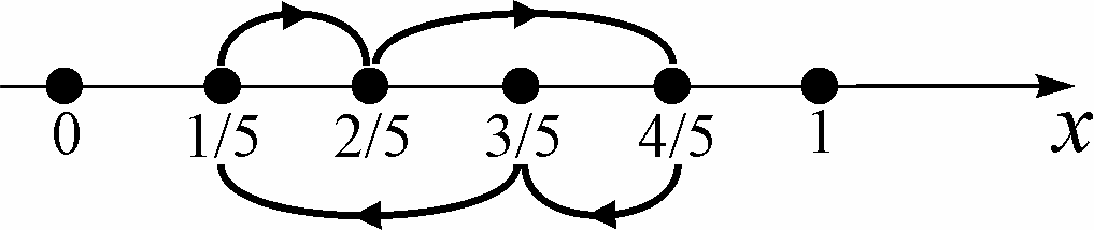
\includegraphics[]{fig/lect1/1}
 	\caption{Полутраектория системы \eqref{eq:1.4} с начальным условием $x(0)=1/5$}
 	\label{fig:1.1}
\end{figure}

% subsubsection динамические_системы_с_дискретным_временем (end)

\subsection{Динамические системы с диссипацией} % (fold)
Рассмотрим динамическую систему \eqref{eq:1.5}  и введем для неё понятие шара диссипации. Говорят, что гладкая поверхность $S=\{\phi(x) = 0 \}$ будет трансверсальной к векторному полю $\vec F (\vec x) $, если скалярное произведение
\begin{equation}
	\qty(\grad \phi(\vec x), \vec F(\vec x)) \neq 0 \qquad \forall \vec x \in S,
\end{equation}
где 
\begin{equation}
	\grad \phi(\vec x) = \qty(\pdv{\phi_1}{x_1},\pdv{\phi_2}{x_2},\dots, \pdv{\phi_m}{x_m})
\end{equation}
Если $S$ топологическая сфера, т.е. граница топологического шара $D$, то шар $D$ называется гаром диссипации, если
\begin{equation}
	\qty(\grad \phi(\vec x), \vec F(\vec x)) < 0 \qquad \forall \vec x \in S,
\end{equation}
Это означает, что векторное поле $\vec F(\vec x)$ на $S$ ориентировано внутрь $D$ (рис. \ref{fig:1.2}). Очевидно, что траектории, входящие в $D$, остаются в нем навсегда. Такие динамические системы называются диссипативными. Наибольшее внимание в нашем курсе будет уделено именно таким динамическим системам, описывающим процессы в физических системах при учете различных потерь. 

\begin{figure}[h!]
	\centering
	
\includegraphics[]{fig/lect1/2}
	\caption{Качественное представление шара диссипации $D$}
	\label{fig:1.2}
\end{figure}


\definition{
\label{def:1.1}
Система \eqref{eq:1.5} называется диссипативной, если существует шар диссипации $D$, такой, что для любой начальной точки $\vec x_0 \in \R^n$: $G^t \vec x_0 \in D$ для некоторого $t>0$.
}

Заметим, что существуют и другие определения диссипативных систем (например, иногда требуют, чтобы $\div \vec F < 0$), но мы будем использовать определение \ref{def:1.1}. 

При исследовании диссипативных систем важную поль играет понятие так называемой поглощающей области.

\definition{\label{def:1.2}
Компактная область $D$ является поглощающей, если 
\begin{equation}
	G^t D \subset \mathrm{Int} D \text{ для } t>0,
\end{equation}}
где $\mathrm{Int} D$ -- внутренняя часть D.

Например, для ДС с дискретным временем вида
\begin{equation}
	\bar x = 3x(1-x)= f(x)
\end{equation}
интервал $[\frac15, \frac45]$ является поглощающей область. Действительно, поскольку 
\begin{equation}
	f\qty(\frac15)=f\qty(\frac45)=\frac{12}{25},\quad f\qty(\frac12)=\frac34,
\end{equation}
то 
\begin{equation}
	f\qty(\qty[\frac15,\frac45])= \qty[\frac{12}{25}, \frac34]\subset \qty(\frac15,\frac45)
\end{equation}
% subsubsection динамические_системы_с_диссипацией (end)
% subsection динамические_системы (end)

\section{Аттракторы} % (fold)

Для систем с диссипацией очень естественно различать переходные процессы и установившиеся процессы или режимы. Базовой чертой установившегося процесса является то, что он «забывает» начальное состояние и не зависит от него. Это означает, что после конечного временного интервала, соответствующего переходному процессу, каждая положительная
полутраектория попадает в малую окрестность некоторого инвариантного множества – <<аттрактора>> (от англ. attract – привлекать, притягивать). Существует несколько определений \href{https://ru.wikipedia.org/wiki/%D0%90%D1%82%D1%82%D1%80%D0%B0%D0%BA%D1%82%D0%BE%D1%80}{аттрактора} (аттрактор Милнора,
статистический аттрактор и др.). Приведем здесь одно из них, которое на наш взгляд наиболее соответствует задачам настоящего курса.
\definition{\label{def:1.3}
Пусть $D$ поглощающая область динамической системы $\qty(G^t, X)$, тогда множество 
\begin{equation}
	A= \bigcap\limits_{t\geq0} G^t D
\end{equation}
называется \textbf{максимальным аттрактором} в $D$.
}
\definition{\label{def:1.4}
Инвариантное множество $A$ является аттрактором, если
существует поглощающая область $D$, для которой $A$ – максимальный аттрактор.
}
Ясно, что максимальный аттрактор зависит от поглощающей области, и может содержать другие аттракторы. Примерами простейших аттракторов являются устойчивые состояния равновесия и неподвижные точки.

% subsection аттракторы (end)

\section{Структурная устойчивость динамических систем} % (fold)
Очевидно, что динамическая система, описывающая поведение любой
реальной системы, должна зависеть от параметров. Рассмотрим, например, систему \eqref{eq:1.5}, зависящую от некоторого набора параметров
\begin{equation}
	\label{eq:1.8}
	\vec {\dot x} = \vec F(\vec x, \vec \mu), \mu \in \R^k,
\end{equation}
где $\mu$ - вектор параметров. Возникает вопрос: нельзя ли обойтись без методов теории колебаний и сделать необходимые нам расчеты динамики системы \eqref{eq:1.8} напрямую, например, численно, используя современные компьютеры и численные методы? Предположим, что мы можем строить приближенно решение системы с любыми начальными условиями. Пусть мы построили какое
– либо решение на некотором временном интервале. Что можно сказать о поведении всей системы, исходя из полученной информации об одном решении? Очевидно – ничего, поскольку в реальных системах начальные условия почти всегда произвольны. Поэтому перебор даже очень большого числа начальных условий не решает полностью задачу, т.к. поведение системы  при оставшихся начальных условиях остается неясным. Кроме того, задачу
усложняет и то, что реальные системы зависят от параметров. Следовательно, используя численное моделирование, мы можем в лучшем случае сказать о  поведении реальной системы только при некоторых значениях параметров и
начальных условий.

Таким образом, для конструирования каких-либо устройств, приборов,
изучения свойств реальных объектов необходимо исследовать не одно какое–либо частное решение системы, а \textbf{целый класс моделей} . Для решения этой
сложной задачи в теории колебаний развивается подход, включающий
следующие базовые положения:
\begin{itemize}
	\item изучать не все траектории системы, а только избранные (в некотором смысле особенные) и находить параметры, при которых такие траектории существуют;
	\item поведение траекторий системы при других значениях параметров изучать, как правило, лишь \textbf{качественно}. 
\end{itemize}

Очевидно, что в динамических системах, описывающих движения
реальных систем, ни один из учитываемых нами факторов не может оставаться абсолютно неизменным во времени. Следовательно, динамические системы, вообще говоря, изменяются вместе с входящими в них параметрами. Однако, если эти изменения достаточно малы, то, как показывает практика, реальная
система как бы не замечает этих изменений, то есть качественные черты ее поведения сохраняются. Поэтому, если мы хотим, чтобы динамическая система отображала эту особенность, нужно придать ей свойство \textbf{грубости}. Именно: при малых изменениях параметров должна оставаться неизменной качественная структура разбиения фазового пространства на траектории. Тем самым выделить класс <<грубых>> динамических систем. Грубость динамической
системы можно трактовать как устойчивость структуры разбиения её фазового пространства на траектории по отношению к малым изменениям динамической
системы. Поэтому грубые динамические системы часто называют структурно устойчивыми.

А.А. Андронов и Л.С. Потрягин (1937 г.) ввели строгое математическое определение грубости динамических систем с двумерным фазовым пространством. Приведем его здесь для системы
\begin{equation}
	\label{eq:1.9}
	\dot x = P(x,y), \quad \dot y = Q(x,y),
\end{equation}
где $P$ и $Q$ -- гладкие функции, а система \eqref{eq:1.9} является диссипативной с шаром диссипации $D$
\definition{\label{def:1.5}
Система \eqref{eq:1.9} называется грубой (структурно устойчивой), если существует такое малое число $\delta>0$m что \textbf{все} динамические системы вида 
\begin{equation}
	\label{eq:1.10}
	\dot x= P(x,y) + p(x,y), \quad \dot y = Q(x,y) + q(x,y),
\end{equation}
в которых аналитические функции $p(x,y)$ и $q(x,y)$ удовлетворяют неравенству
\begin{equation}
	\label{eq:}
	\abs{p(x,y)} + \abs{q(x,y)} +\abs{\pdv{p}{x}} +
	\abs{\pdv{q}{x}}  + \abs{\pdv{p}{y}} + \abs{\pdv{q}{y}} < \delta,
\end{equation}
имеют такую же структуру разбиения $D$ на положительные полутраектории, что и система \eqref{eq:1.9}
}

Совершенно ясно, что не при всяком изменении параметра грубость
динамической системы сохраняется. Можно так поменять параметр, что
произойдет принципиальное изменение фазового портрета. Переход от одной грубой динамической системы к другой происходит через негрубую динамическую систему. Значение параметра, при котором динамическая система является негрубой, называется \textbf{бифуркационным}. Требование грубости для автономных систем второго порядка, являясь естественным с точки зрения приложений, существенно упрощает возможные структуры разбиения фазовой плоскости на траектории. Каждая из этих структур определяется конечным числом особых фазовых траекторий. Что это за траектории речь пойдет ниже в курсе теории колебаний

Заметим, что прямое перенесение, приведенного выше определения
грубости, на случай многомерных (размерность фазового пространства три и выше) динамических систем оказалось невозможным. Было установлено, что существуют многомерные системы, содержащие только неустойчивые траектории, а в пространстве динамических систем существуют целые области
негрубых систем. Поэтому теория грубых многомерных динамических систем строится иначе, чем в двумерном случае. Мы обратимся к этому вопросу позднее.
% subsection структурная_устойчивость_динамических_систем (end)

%\section{Контрольные вопросы и задания} % (fold)
%\begin{enumerate}
	%\item Найти 2- и 3-периодические траектории ДС \eqref{eq:1.7}.
	%\item Показать, что система $\dot x = x- x^3$ является диссипативной.
	%\item Найти поглощающую область для отображения $\bar x= 3.1x(1-x)$
%\end{enumerate}
% subsection контрольные_вопросы_и_задания (end)



\newpage
\chapter{Динамические системы на прямой}
\label{lect2}
	%!TEX root = ../lections.tex
	Динамические системы с одномерным фазовым пространством – системы
на прямой являются простейшим видом непрерывных динамических систем с
конечномерным фазовым пространством. Сами по себе такие модели
описывают поведение достаточно простых реальных систем. Например,
изменение заряда $q$ в простейшем $RC$-контуре (рис. \ref{fig:2.1}), содержащем конденсатор с сегнетоэлектриком (вещество с нелинейной зависимостью поляризации от приложенного электрического поля).
\begin{figure}[h!]
	\begin{minipage}{0.49\linewidth}
		\centering
		\includegraphics[width=\linewidth]{example-image-a}
		% \caption{(a)}
	\end{minipage}
	\hfill
	\begin{minipage}{0.49\linewidth}
		\centering
		\includegraphics[width=\linewidth]{example-image-a}
		% \caption{(b)}
	\end{minipage}
	\caption{(a) ~ $RC$-контур; (b) нелинейная характеристика конденсатора с диэлектриком}
	\label{fig:2.1}
\end{figure}

	
Однако, с методической точки зрения эти системы чрезвычайно важны,
поскольку дают наглядное и ясное представление о базовых идеях и подходах
теории колебаний.
\section{Качественный подход} % (fold)
Во многих случаях качественные (геометрические) представления о
динамике нелинейных систем бывают более полезны, чем даже точное решение
системы. Поясним это на простом примере. Рассмотрим уравнение
\begin{equation}
	\label{eq:2.1}
	\dot x = x- x^2
\end{equation}

Очевидно, что $x=0$ и $x=1$ является решениями \eqref{eq:2.1}. Найдем остальные решения. Считая, что $x\neq 0;\,1$, разделим переменные в \eqref{eq:2.1}
\begin{equation}
	\label{eq:2.2}
	\frac{\dd{x}}{x-x^2}= \dd{t}
\end{equation}
Интегрируя \eqref{eq:2.2}, получаем 
\begin{equation}
	\label{eq:2.3}
	\ln|x| - \ln|1-x|+C=t,		
\end{equation}
где $C=\const$. Рассмотрим решение уравнения \eqref{eq:2.1}, удовлетворяющее начальному условию: $x(0)=x_0,$ где $x_0\neq 0\,1$. Из \eqref{eq:2.3} находим, что этому начальному условию отвечает постоянная
\begin{equation}
	\label{eq:}
	C=\ln|1-x_0| - \ln|x_0|
\end{equation}
и соответствующее решение имеет вид
\begin{equation}
	\label{eq:2.4}
	\ln\abs{\frac{x}{x_0}} - \ln\abs{\frac{1-x}{1-x_0}}=t
\end{equation}
Выражение \eqref{eq:2.4} задает точное решение рассматриваемой задачи. Давайте попробуем получить из \eqref{eq:2.4} ответы на следующие вопросы:
\begin{enumerate}
	\item Пусть $x_0=\frac12$. Как изменяется переменная $x(t)$ при $t>0$ и, в частности, какое предельное значение она принимает при $t \rightarrow +\infty$?
	\item Как ведёт себя $x(t)$ при $t \rightarrow + \infty$ при различных значениях $x_0$?
\end{enumerate}

Конечно, из \eqref{eq:2.4} ответить на эти вопросы можно, но это требует некоторых дополнительных рассуждений и выкладок. Давайте теперь для ответа на эти вопросы привлечем базовое понятие теории колебаний -- фазовое пространство. Для системы \eqref{eq:2.1} фазовым пространством является числовая прямая $\R^1$. Отметим на $\R^1$ значения $x=0$ и $x=1$. В этих точках $\dot x=0$ и, следовательно, эти значения не изменяются во времени. Из \eqref{eq:2.1} легко найти знак $\dot x$ во всех интервалах прямой $\R^1$, определяемых значениями $x=0$ и $x=1$, и тем самым установить направление движения фазовых траекторий. Отсюда, принимая во внимание структуру разбиения фазовой прямой на траектории, легко дать ответы на поставленные вопросы.

\begin{figure}[h!]
	\centering
	\includegraphics[width= 0.5\linewidth]{example-image-a}
	\caption{Фазовая прямая системы \eqref{eq:2.1}}
	\label{fig:2.2}
\end{figure}





\begin{enumerate}
	\item Траектория с начальным условием $x_0=\frac12$ при $t \rightarrow + \infty$ асимптотически стремится к значению $x=1$.
	\item Все траектории с начальными условиями $x_0>0$ ($x_0\neq1$) при $t \rightarrow + \infty$ асимптотически стремятся к значению $x=1$ , а при $x_0<0$ переменная $x(t)$ неограниченно убывает, т.е. $x(t) \rightarrow - \infty$. 
\end{enumerate}

Рассмотренный пример показывает, что в фазовом пространстве существуют значения $x$, которые остаются неизменными при любом $t$ -- это так называемые состояния равновесия (см. лекцию \ref{lect1}, раздел \ref{subsubsec:1.2.1}). С теоретической точки зрения любое состояние равновесия представляет собой классический геометрический объект -- точку. В системе \eqref{eq:2.1} к точке $x=1$ траектории системы асимптотически приближаются при $t \rightarrow + \infty$ и поэтому это состояние равновесия логично называть устойчивым, а от точки $x=0$ траектории, наоборот, удаляются при увеличении $t$ и его, поэтому, называют неустойчивым (строгое определение устойчивости состояний равновесия мы дадим позднее).

% subsection качественный_подход (end)

\section{Грубые состояния равновесия} % (fold)
\label{subsec:2.2}

Рассмотрим динамическую систему на прямой общего вида
\begin{equation}
	\label{eq:2.5}
	\dot x = F(x, \vec \mu) =0,
\end{equation}
где $x \in \R^1$, $\vec \mu \in \R^m$ -- вектор параметров. Будем считать, что $F(x)$ -- взаимнооднозначная функция, обеспечивающая выполнение теорем существования и единственности решений. Очевидно, что состояние равновесия системы \eqref{eq:2.5} определяются уравнением
\begin{equation}
	\label{eq:2.6}
	F(x, \vec \mu) =0.
\end{equation}
Пусть $x=x^*(\vec \mu)$ -- одно из решений уравнения \eqref{eq:2.6}. Найдем условия локальной устойчивости состояния равновесия $x^*(\vec \mu)$. Пусть $\xi(t) = x - x^*(\vec \mu)$ -- малое возмущение, тогда из системы \eqref{eq:2.5} имеем
\begin{equation}
	\label{eq:}
	\dot \xi = F(x^*(\vec \mu)+ \xi, \vec \mu) = F(x^*(\vec \mu), \vec \mu) + F^\prime_x (x^*(\vec \mu), \mu) \xi + \dots
\end{equation}
или
\begin{equation}
	\label{eq:2.7}
	\dot \xi = F^\prime_x (x^*(\vec \mu), \mu) \xi + \dots
\end{equation}

Если $F^\prime_x (x^*(\vec \mu), \mu) \neq 0$, то в малой окрестности $x=x^*(\vec \mu)$ в  \eqref{eq:2.7} можно ограничиться лишь линейным слагаемым по $\xi$, т.е. вместо \eqref{eq:2.7} рассмотреть линейное уравнение (эта процедура называется линеаризацией, рамки применения которой мы обсудим позднее) вида
\begin{equation}
	\label{eq:2.8}
	\dot x = \lambda(\vec \mu) \xi, \text{ где } \lambda(\vec \mu) = F^\prime_x (x^*(\vec \mu), \mu).
\end{equation}
Поскольку общее решение уравнения \eqref{eq:2.8} имеет вид
\begin{equation}
	\label{eq:}
	\xi(t) = Ce^{\lambda(\vec \mu)t},
\end{equation}
где $C=\const$, то при условии $\lambda(\vec \mu)<0$ возмещение $\xi(t) \rightarrow 0$ при $t \rightarrow + \infty$ и состояние равновесия $x^*(\vec \mu)$ будет устойчивым, а если $\lambda(\vec \mu) > 0 $, то $\xi(t)$ растут и $x^*(\vec \mu)$ будет неустойчивым. Коэффициент $\lambda (\vec \mu)$ называется ляпуновским характеристическим показателем. Условия устойчивости допускают простую геометрическую интерпретацию. Состояние равновесия $x^*(\vec \mu)$ является локально устойчивым, если производная функции $F(x, \vec \mu)$ по точке $x^*(\mu)$ отрицательная и неустойчиво, если $F^\prime(x^*(\vec \mu), \mu)>0$ (рис. \ref{fig:2.3}) 

\begin{figure}[h!]
	\centering
	\begin{minipage}{0.49\linewidth}
		\centering
		\def\svgwidth{\linewidth}
		\input{fig/fig2_3a.pdf_tex}
		% \caption{(a)}
		\label{fig:2.3a}
	\end{minipage}
	\hfill{}
	\begin{minipage}{0.49\linewidth}
		\centering
		\def\svgwidth{\linewidth}
		\input{fig/fig2_3b.pdf_tex}
		% \caption{(b)}
		\label{fig:2.3b}
	\end{minipage}
	\caption{Поведение функций $F(x, \vec \mu)$ в окрестности точки $x=x^*(\vec \mu)$ в случае устойчивого (а) и неустойчивого (b) состояний равновесия.}
	\label{fig:2.3}
\end{figure}

Ясно, что в обоих случаях малые изменения правой части системы \eqref{eq:2.5} не могут привести к исчезновению и смене устойчивости состояния равновесия $x^*(\vec \mu)$. Следовательно, условие грубости состояний равновесия на прямой имеет вид $\lambda(\vec \mu) \neq 0$, а буфуркационные значения параметров определяются уравнением $\lambda(\vec \mu^*)=0$. Таким образом, динамическая система \eqref{eq:2.5} на прямой будет грубой (структурно устойчивой), если для всех состояний равновесия выполнено условие $\lambda_i (\vec \mu) \neq 0$.

% subsection грубые_состояния_равновесия (end)
\section{Бифуркации состояний равновесия} % (fold)
\subsection{Двукратное равновесие}

Бифуркация двукратное равновесие определяет один из базовых динамических механизмов рождения и исчезновения состояний равновесия. Рассмотрим систему следующего вида
\begin{equation}
	\label{eq:2.9}
	\dot x = \mu  + x^2,	
\end{equation}
где $\mu \in \R^1$. Анализ динамики системы \eqref{eq:2.9} прост и представлен на рис. \ref{fig:2.4}
\begin{figure}[h!]
	\centering
	\includegraphics[width=\linewidth]{example-image-a}
	\caption{Разбиение фазовой прямой на траектории для системы \eqref{eq:2.9} при различных значениях параметра $\mu$}	
	\label{fig:2.4}	
\end{figure}
Он показывает, что при $\mu =0 $ состояние равновесия $x=0$ является негрубым, поскольку любое сколь угодно малое изменение параметра $\mu$ приводит к принципиальному изменению структуры фазовой прямой. Такое состояние равновесия называется двухкратным, так как при его разрушении на фазовой прямой появляются два грубых состояния равновесия. 

Совершенно аналогично для системы
\begin{equation}
	\label{eq:2.10}
	\dot x= \mu - x^2, \quad \mu \in \R^1	
\end{equation}
получаем разбиение фазовой прямой, представленное на рис.
\begin{figure}[h!]
 	\centering
 	\includegraphics[width=\linewidth]{example-image-a}
 	\caption{Фазовая прямая системы \eqref{eq:2.10} для различных значений параметра $\mu$ }
 	\label{fig:2.5}
 \end{figure} 

 Представленны на рисунках \ref{fig:2.5}-\ref{fig:2.4} результаты удобно представить в виде так называемых бифуркационных диаграмм, представляющих собой зависимость стационарных состояний системы от параметра $\mu$ , который принято называть контрольным параметром. Эти диаграммы для систем \eqref{eq:2.9}-\eqref{eq:2.10} изображены на рис.\ref{fig:2.6}a и b соответственно.

 \begin{figure}[h!]
 	\centering
 	\begin{minipage}{0.49\linewidth}
 		\centering
 		\includegraphics[width=\linewidth]{example-image-a}
 		(a)
 		\label{fig:2.6a}
 	\end{minipage}
 	\hfill
 	\begin{minipage}{0.49\linewidth}
 		\centering
 		\includegraphics[width=\linewidth]{example-image-a}
 		(b)
 		\label{fig:2.6b}
 	\end{minipage}
 	\caption{ (a) Бифуркационные диаграммы системы \eqref{eq:2.9} и (b) системы \eqref{eq:2.10}. Пунктирной линией указана ветвь неустойчивых, а сплошной -- устойчивых состояний равновесия}
 	\label{fig:2.6}
 	
 \end{figure}

Таким образом, двукратное равновесия -- негрубое состояние равновесия, которые при сколь угодно малом изменении параметра либо распадается на два грубых, либо исчезает.

\subsection{Понятие о нормальной форме} % (fold)

В определенном смысле системы \eqref{eq:2.9} и \eqref{eq:2.10} описывают все возможные бифуркации двукратных состояний равновесия на прямой и поэтому их называют нормальной формой для этой бифуркации. Другими словами, если какая-либо система прямой имеет двухкратное равновесие, то в окрестности этой точки поведение системы можно описать с помощью уравнения \eqref{eq:2.9} или \eqref{eq:2.10}. Действительно, пусть при $\mu = \mu_0$ система \eqref{eq:2.5} имеет двухкратное равновесия $x=x_0$. Раскладывая правую часть \eqref{eq:2.5} в ряд Тейлора, получим
\begin{gather}
	\dot x = F(x, \mu) = F(x_0, \mu_0)  + (x-x_0) \pdv{F}{x} \eval_{(x_0,\mu_0)} +
	(\mu- \mu_0)\pdv{F}{\mu} \eval_{(x_0,\mu_0)} + \\ 
	\frac12 (x-x_0)^2 \pdv[2]{F}{x} \eval_{(x_0,\mu_0)} + \dots
	\label{eq:2.11}
\end{gather}
Поскольку
\begin{equation}
	\label{eq:}
	F(x_0, \mu_0) = 0, \quad \lambda(\mu_0) = \pdv{F}{x}\eval_{x_0, \mu_0} = 0 ,
\end{equation}

 то \eqref{eq:2.11} можно переписать в следующем виде
 \begin{equation}
 	\label{eq:2.12}
 	\dot x = a(\mu - \mu_0) + b (x-x_0)^2 + \dots ,
 \end{equation}
 где $a = \pdv{F}{x}\eval_{(x_0, \mu_0} $, $b =\frac12 \pdv[2]{F}{x}\eval_{(x_0, \mu_0)}$.
 Очевидно, что уравнение \eqref{eq:2.12} путем введения новых переменных и параметра принимает вид \eqref{eq:2.9} или \eqref{eq:2.10}.
% subsubsection понятие_о_нормальной_форме (end)
\subsection{Транскритическая бифуркация} % (fold)

Существует значительное число задач, в которых число состояний
равновесия при изменении параметров сохраняется, но их устойчивость
меняется. Такая бифуркация носит название транскритической или смены
устойчивости состояния равновесия. Нормальная форма для транскритической
бифуркации задается уравнением
\begin{equation}
	\label{eq:2.13}
	\dot x = \mu x -x^2
\end{equation}
или уравнением 
\begin{equation}
	\label{eq:2.14}
	\dot x = \mu x+ x^2	
\end{equation}

Динамика уравнений \eqref{eq:2.13}, \eqref{eq:2.14} в зависимости от управляющего параметра $\mu$ представлена на рис.\ref{fig:2.7}a и \ref{fig:2.7}b соответственно

\begin{figure}[h!]
	\centering
	\begin{minipage}{0.49\linewidth}
		\centering
		\includegraphics[width=\linewidth]{example-image-a}
		(a)
		\label{fig:2_7a}
	\end{minipage}
	\hfill
	\begin{minipage}{0.49\linewidth}
		\centering
		\includegraphics[width=\linewidth]{example-image-a}
		(b)
		\label{fig:2_7b}
	\end{minipage}
	\caption{Разбиение фазовой прямой на траектории для системы \eqref{eq:2.13} и \eqref{eq:2.14} соответственно}.
	\label{fig:2.7}
	
\end{figure}

Принимая во внимание рузультаты представленные на рис.\ref{eq:2.7}, устанавливаем вид буфурцационных диаграмм для систем \eqref{eq:2.13} и \eqref{eq:2.14} (см. рис.\ref{fig:2.8})  
\begin{figure}[h!]
	\centering
	\begin{minipage}{0.49\linewidth}
		\centering
		\includegraphics[width=\linewidth]{example-image-a}
		(a)
		\label{fig:2_8a}
	\end{minipage}
	\hfill
	\begin{minipage}{0.49\linewidth}
		\centering
		\includegraphics[width=\linewidth]{example-image-a}
		(b)
		\label{fig:2_8b}
	\end{minipage}
	\caption{Бифуркационные диаграммы системы \eqref{eq:2.13} (a) и системы \eqref{eq:2.14} (b). Ветвь устойчивых состояний равновесия отмечена сплошной лнией, а неустойчивых -- пунктирной.}
	\label{fig:2.8}
	
\end{figure}
% subsubsection транскритическая_бифуркация (end)

\subsection{Трехкратное равновесие} % (fold)

Эта бифуркация типична для систем, обладающих симметрией.
Например, многие физические задачи имею пространственную симметрию
между левым и правым направлениями. В таких системах состояния
равновесия рождаются и исчезают парами. Нормальная форма бифуркации
трехкратное равновесие определяется уравнениями

\begin{equation}
	\label{eq:2.15}
	\dot x = \mu x - x^3,
\end{equation}
\begin{equation}
	\label{eq:2.16}
	\dot x = \mu x + x^3. 
\end{equation}

Нетрудно видеть, что уравнения \eqref{eq:2.15} и \eqref{eq:2.16} инвариантны относительно
преобразования $x \rightarrow -x$. Исследование динамики уравнения \eqref{eq:2.15} представлено
на рис.\ref{fig:2.9}.

\begin{figure}[h!]
	\centering
	\includegraphics[width=\linewidth]{example-image-a}
	\caption{Разбиение фазовой прямой на траектории для системы \eqref{eq:2.15} при различных значениях параметра $\mu$}
	\label{fig:2.9}
\end{figure}


Обратим внимание на то, что в момент бифуркации, т.е. при $\mu=0$, ляпуновский характеристический показатель $\lambda(0) = 0$ , а само состояние равновесия, несмотря на это является устойчивым. Исследование уравнения \eqref{eq:2.16} проводится аналогично предыдущему и мы предлагаем читателю провести его самостоятельно. Представим здесь лишь соответствующую бифуркационную диаграмму (см.рис. \ref{fig:2.10}b).
\begin{figure}[h!]
    \centering
    \includegraphics[width=0.8\linewidth]{example-image-a}
    \caption{Буфуркационные диаграммы системы \eqref{eq:2.15}(а) и системы \eqref{eq:2.16}(b).
    Ветвь устойчивых состояний равновесия отмечена сплошной линией, а неустойчивых -- пунктирной.}
    \label{fig:2.10}
\end{figure}
% subsubsection трехкратное_равновесие (end)
% subsection бифуркации_состояний_равновесия (end)
\section{Система на окружности}%
Рассмотрим  уравнение первого порядка следующего вида
\begin{equation}
    \label{eq:2.17}
    \dot \phi = F(\phi) , \text{ где } F( \phi + 2 \pi) = F( \phi ) 
\end{equation}
Уравнения такого вида возникают при описании динамики реальных систем, у которых переменная состояния изменяется циклически. Например, простейшая безфильтровая система фазовой автоподстройки (см. лекцию 4, уравнение \eqref{eq:4.23}) описывается уравнением $\dot \phi + \sin \phi = \gamma$. В силу периодичности правой части \eqref{eq:2.17} по $\phi$ её фазовым пространством является окружностью $S^1$. Поясним основные свойства таких систем на следующем примере. Рассмотрим уранение
\begin{equation}
    \label{eq:2.18}
    \dot \phi = \omega - a \sin \phi   , 
\end{equation}
где $a$ и $ \omega$ -- параметры, $a\geq0$, $\omega=0$ . При $a=0$ общее решение уравнения \eqref{eq:2.17} имеет вид
\begin{equation}
    \label{eq:}
    \phi = \omega t + \phi_0, \quad \phi_0= \const
\end{equation}
и описывает равномерное вращение изображающей точки по окружности $S^1$. Исследование системы \eqref{eq:2.18} образуется двукратное равновесие, которое при изменении параметров либо распадается на два грубых $(a > \omega)$ либо исчезает  $(a<\omega)$ в \eqref{eq:2.18} происходят вращательные движения, однако эти движения, однако эти движения неравномерны, поскольку скорость $\dot \phi$ не является постоянной (наибольшая скорость достигается при $\phi = - \frac{\pi}{2},$ а минимальная при  $\phi = \frac{\pi}{2}$ ). При $a>\omega$ на окружности $S^1$ существует два грубых состояния равновесия: $\phi = \phi_1 = \arcsin(\omega/a)$ и $\phi = \phi_2= \pi - \arcsin(\omega/a)$. Состояние равновесия $\phi=\phi_1$ -- устойчивое, а $\phi = \phi_2$ -- неустойчивое.




\newpage
\chapter{Устойчивость состояний равновесия. Классификация состояний равновесия двумерных линейных
систем}
\label{lect3}
	%!TEX root = ../lections.tex
\graphicspath{{fig/lect3/}}
На предыдущей лекции мы познакомились со свойствами динамических систем на прямой. Было показано, что поведение таких систем определяется также состояниями равновесия и выбором начальных условия. Состояния равновесия также играют чрезвычайно важную роль и в динамике многомерных систем, поскольку они описывают стационарные состояния реальных систем. Важнейшим свойством состояний равновесия является их устойчивость. Термин <<устойчивость>> настолько широко распространён не только в научной литературе, но и в повседневной жизни, что его смысл интуитивно ясен даже людям далёким от науки. Например, вот такое определение <<устойчивый>> дается в словаре русского языка С.И.Ожегова:
\begin{enumerate}
    \item Стоящий твёрдо, не колеблясь, не падая.
    \item Не поддающийся, не подверженный колебаниям, стойкий, твёрдый
\end{enumerate}
Хотя, конечно, с физико-математической точки зрения, это определение нельзя назвать строгим,  одна из важнейших и типичных характеристик устойчивости в нём содержится. Именно -- сохранение исходного состояния системы при некоторых отклонениях (возмущениях). Однако, лишь одной этой характеристики недостаточно для построения строгого определения устойчивости, приемлемого для широкого круга практических задач. Свойство возвращаемости системы в исходное состояние является слишком строгим и оставляет <<за бортом>> широкий класс систем, для которых характерно более слабое проявление устойчивости -- сохранения своего положения в малой окрестности исходного состояния. Действительно, рассмотрим поведение массивного шарика в желобе, состоящем из двух ямок (рис. \ref{fig:3.1}). Очевидно, что в этой системе возможно  существование трёх состояний   равновесия:
$A$, $B$ и $C$. 
\begin{figure}[h!]
    \centering
    \includegraphics[width=0.8\linewidth]{example-image-a}
    \label{fig:3.1}
    \caption{Колебания массивного шарика в желобе. }
\end{figure}
При сколь угодно малых отклонениях шарика от точки В, он начинает
двигаться и покидает окрестность этой точки. Поэтому вполне логичным было
бы назвать такое состояние равновесия неустойчивым. Совершенно иначе ведёт
себя шарик, если изначально он покоился в точке А или С. Получив начальное
отклонение, шарик начнёт двигаться с уменьшающейся за счёт трения
скоростью и придёт в одно из этих состояний равновесия. Причём, в
зависимости от величины отклонения шарик может сохранить своё начальное
состояние равновесия, а может изменить его на противоположное.
Следовательно, состояние равновесия может быть устойчивым по отношению к
одним отклонениям и в тоже время быть неустойчивым по отношению к
другим. Предположим теперь, что трение в жёлобе пренебрежимо мало. Как
известно, в этом случае при малых отклонениях от точек А и С шарик будет
совершать периодические колебания в их окрестности. Поскольку эти
колебания происходят в окрестности точек А и С, состояние системы
существенно не меняется и такое поведение шарика можно отнести к
устойчивому. Как мы увидим ниже, отмеченные выше свойства состояний
равновесия являются общими и лежат в основе строгого определения
устойчивости состояний равновесия.

Основы теории устойчивости были заложены в работах великого
русского математика и механика А.М. Ляпунова. В 1892 году в Харькове он
представил к защите докторскую диссертацию, которая была опубликована год
спустя. Идеи и подходы, заложенные в этой работе, оказались настолько
плодотворными, что до сих пор являются актуальными и востребованными.
Изложим положения определения теории устойчивости, принадлежащие
Ляпунову.

\section{Определение устойчивости состояний равновесия}%


Рассмотри автономную динамическую систему
\begin{equation}
    \label{eq:3.1}
    \dot {\vec{x}} =  \vec{F}(\vec{x}), \vec{x} \in \R^n,   \vec{F}: \R^n \rightarrow \R^n
\end{equation}
Как мы уже знаем (см. лекцию \ref{lect2}), состояние равновесия определяется из условия равенства нулю всех производных по времени. Следовательно, состояние равновесия системы \eqref{eq:3.1} являются решениями следующей системы
\begin{equation}
    \label{eq:3.2}
    \vec F(\vec x) = 0 . 
\end{equation}
Пусть $\vec x= \vec x^*$ -- одно из решений системы \eqref{eq:3.2}. Для оценки близости состояния равновесия и накладываемых на систему возмущений (отклонений) введём в фазовом пространстве системы    \eqref{eq:3.1} норму. В качестве нормы мы будем использовать евклидову длину вектора, т.е.
\begin{equation}
    \label{eq:}
    \norm {x}=\qty( \sum\limits_{i=1}^n x_i^2) ^{\frac12}.
\end{equation}
Не останавливаясь здесь подробно, отметим лишь, что существуют и другие способы задания нормы. При этом сходимость в одной из норм автоматически означает сходимость и в смысле других норм.

\definition{\label{def:3.1} Состояние равновесия $\vec x = \vec x^*$ системы \eqref{eq:3.1} называется устойчивым (в смысле Ляпунова), если для такого $ \epsilon > 0$ (как бы мало оно ни было) можно указать $\delta (\epsilon) > 0$ такое, что из неравенства
\begin{equation}
    \label{eq:3.3}
    \norm{\vec x^* - \vec x(t_0)} < \delta
\end{equation} 
следует неравенство
\begin{equation}
    \label{eq:3.4}
    \norm{\vec x^* - \vec x(t)} < \epsilon
\end{equation}
при $t\geq t_0$.}

Если же найти такой $\delta$ невозможно, состояние равновесия $\vec x = \vec x^*$ называется неустойчивым. Заметим, что из условий \eqref{eq:3.3} и \eqref{eq:3.4} следует, что всегда можно выбрать число $\delta$ из условия $\delta \leq \epsilon $, а число $\epsilon$ задает область допустимых возмущений (отклонений).

\definition{\label{def:3.2} Состояние равновесия $\vec x = \vec x^*$ системы \eqref{eq:3.1} называется асимптотически устойчивым, если оно устойчиво по Ляпунову и для всех решений $\vec x(t)$ системы \eqref{eq:3.1}, удовлетворяющих условию \eqref{eq:3.3}, выполняется равенство
\begin{equation}
  \label{eq:3.5}
  \lim\limits_{t \rightarrow +\infty} \norm{\vec x(t) - \vec x} =0
\end{equation}}
Рис. \ref{fig:3.2} иллюстрирует определения \ref{def:3.1} и \ref{def:3.2}. Устойчивость по Ляпунову состояния равновесия $\vec x = \vec x^*$ означает, что достаточно близкие к нему в любой начальный момент $t=t_0$ решения $\vec x(t)$ целиком останутся в сколь угодно узкой $\epsilon$-трубке около значения $\vec x = \vec x^*$ (рис. \ref{fig:3.2}a). В фазовом пространстве устойчивость по Ляпунову, в выбранной нами норме, означает, что любая траектория системы \eqref{eq:3.1} с начальными условиями внутри сферы радиуса $\epsilon$ (рис. \ref{fig:3.2}b) ни при каких $t>t_0$ не достигают сферы радиуса $\epsilon$. В случае асимптотической устойчивости, кроме того, требуется стремление траекторий к состоянию равновесия (рис. \ref{fig:3.2}c) 

Из определения \ref{def:3.2} следует, что асимптотическая устойчивость состояний равновесия зависит от величины начальных возмущений. В связи с этим различают устойчивость в \textbf{малом}, в \textbf{большом} и в \textbf{целом}. Состояние равновесия называется ассимптотически устойчивым в целом, если определение \ref{def:3.2} выполняется при любых начальных условиях. Если же определение \ref{def:3.2} выполняется для начальных условий из некоторой ограниченной области, то состояние равновесия, то состояние равновесия называется асимптотически устойчивым в большом (в этой области). Наконец, если определение \ref{def:3.2} справедливо для начальных  возмущений из сколь угодно малой окрестности состояния равновесия, что оно называется асимптотически устойчивым в малом.
Для систем, у которых одновременно существует несколько состояний равновесия, существует понятие \textbf{ глобальной асимптотической устойчивости}. Система называется глобально асимптотически устойчивой, если каждая её траектория асимптотически  стремится к какому-либо состоянию равновесия.

\begin{figure}[h!]
        \centering
        \includegraphics[width=0.8\linewidth]{example-image-a}
        \label{fig:3.2}
        \caption{Качественное представление эволюции во времени переменной $x(t)$ в фазовом пространстве в случае устойчивости по Ляпунову (а); примеры поведения траектории $x(t)$ в фазовом пространстве в случае устойчивости по Ляпунову (b) и в случае асимптотической устойчивости состояния равновесия $x^*$ (c) }
\end{figure}

\section{Классификация состояний равновесия линейных систем на плоскости}%
\label{sub:3.2}

Рассмотрим произвольную линейную систему второго порядка 
\begin{equation}
        \label{eq:3.6}
        \begin{cases}
                \dot x_1 = ax_1 + bx_2, \\
                \dot x_2 = cx_1 +dx_2,
        \end{cases}
\end{equation}
где $a, b ,c$ и $d$ -- некоторые параметры. Для удобства изложения простим \eqref{eq:3.6} также в векторной форме
\begin{equation}
        \label{eq:3.7}
        \dot{\vec x} = \vec A \vec x, 
\end{equation}
где
\begin{equation}
        \label{eq:}
        \vec A =
        \begin{pmatrix}
                a & b \\
                c & d
        \end{pmatrix}, \quad 
        \vec x = 
        \begin{pmatrix}
                x_1 \\
                x_2 
        \end{pmatrix}
\end{equation}
Предположим, что $\det \vec A \neq 0$, тогда система \eqref{eq:3.6} имеет единственное состояние равновесия $O(x_1=x_2=0)$. Будем искать решение системы \eqref{eq:3.6} в виде
\begin{equation}
        \label{eq:3.8}
        x_i = C_i e^{ \lambda t}, \quad i=1,2   
\end{equation}
где $C_i$ -- произвольные константы. Подставляя 
\eqref{eq:3.8} в систему \eqref{eq:3.6} получим систему линейных однородных уравнений относительно $C_1$ и $C_2$, которая имеет нетривиальное решение, если её определитель равен нулю, т.е.
\begin{equation}
        \label{eq:3.9}
        \det(\vec A - \lambda E) = \lambda_2 - (a+d) \lambda + ad - bc =0
\end{equation}
Это уравнение называется характеристическим. Обозначим через $\lambda_1$ и $\lambda_2$ корни уравнения \eqref{eq:3.9}. Рассмотрим поведение фазовых траекторий системы \eqref{eq:3.6} для различных значений $\lambda_1$ и $\lambda_2$.

\subsection{Действительные корни}%
\label{ssub:3.2.1}

Предположим, что уравнение \eqref{eq:3.9} имеет действительные корни, удовлетворяющие условиям

\begin{equation}
        \label{eq:3.10}
        \lambda_1\neq \lambda_2, \quad \lambda_{12}\neq 0.
\end{equation}
Покажем, что при этих условиях система \eqref{eq:3.6} с помощью взаимооднозначного преобразования координат может быть приведена к виду
\begin{equation}
        \label{eq:3.11}
        \begin{cases}
                \dot u_1 = \lambda_1 u_1,\\
                \dot u_2 = \lambda_2 u_2.
        \end{cases}
\end{equation}
Система \eqref{eq:3.11} называется нормальной формой уравнений для грубых состояний равновесия линейных двумерных систем. Как мы убедимся ниже,a исследование фазовой плоскости системы \eqref{eq:3.11} представляет собой значительно более простую задачу, чем исследование фазовой плоскости исходной   системы \eqref{eq:3.6}.

Введем в \eqref{eq:3.6} новые переменные
\begin{equation}
        \label{eq:3.12}
        \begin{cases}
                u_1= h_{11} x_1 +h_{12} x_2,\\
                u_2=h_{21} x_1 +h_{22} x_2
        \end{cases}
        ,
\end{equation}
где $h_{ik} (i,k= 1,2)$ -- некоторые, пока неопределенные, коэффициенты. Из \eqref{eq:3.12} и первого уравнения системы \eqref{eq:3.6} имеем
\begin{equation}
        \label{eq:3.13}
        \dot u_1 = h_{11} \dot x_1 + h_{12} \dot x_2 = (h_{11} a + h_{12}c) x_1+ (h_{11} b+ h_{12} d) x_2.
\end{equation}
С другой стороны, из системы \eqref{eq:3.11}
\begin{equation}
        \label{eq:3.14}
        \dot u_1 = \lambda_1(h_{11} x_1 + h_{12} x_2).
\end{equation}
Приравнивая коэффициенты при переменных $x_1$ и $x_{2}$ в \eqref{eq:3.13} и \eqref{eq:3.14}, находим системы для определения $h_{i,k}$ 
\begin{equation}
        \label{eq:3.15}
        \begin{cases}
                h_{11}(a - \lambda_1) + h_{12} c=0,\\
                h_{11} b + h_1(d -\lambda) =0.
        \end{cases}
\end{equation}
Система \eqref{eq:3.15} -- система однородных линейных уравнений отностиельно $h_{11}$ и $h_{12}$. Определитель этой системы равен нулю и, следовательно, система \eqref{eq:3.15} меет нетривиальное решение
\begin{equation}
        \label{eq:3.16}
        \begin{gathered}
                h_{11} = p,~h_{12}= - p\frac{a-\lambda_1}{c}, \quad \text{ если}~ c \neq 0, \\
                h_{11}=p, h_{12} = -  \frac{dp}{d-a},\quad \text{если} ~ c=0, d\neq 0,
        \end{gathered}
\end{equation}
где $p= \const$. Совершенно аналогично устанавливается вид остальных коэффициентов, преобразования \eqref{eq:3.12}
\begin{equation}
        \label{eq:3.17}
        \begin{gathered}
                h_{21}=q , h_{22} = - \frac{q (a- \lambda_2)}{c}, \quad \text{ если } c\neq 0 \\
                h_{21}=0, h_{22}= q, \quad \text{ если } c=0, d\neq a,
        \end{gathered}
\end{equation}
где $q = \const$. Пусть для определённости $p=q=1$. В этом случае искомое преобразование системы \eqref{eq:3.6} к виду \eqref{eq:3.11} имеет следующий вид
\begin{equation}
        \label{eq:3.18}
        \begin{aligned}
               & \begin{cases}
                        u_1 = x_1 - \frac{a- \lambda_1}{c} x_2 \\
                        u_2 = x_1 - \frac{a- \lambda_2}{c} x_2
                \end{cases},
                &\text{ если } c\neq 0 \\
               & \begin{cases}
                       u_1 = x_1 - \frac{b}{d-a} x_2 \\
                       u_2=x_2 
                \end{cases},
                &\text{если } c=0,~ d\neq a.
        \end{aligned}
\end{equation}

Рассмотрим теперь поведение траектории системы \eqref{eq:3.11} на фазовой плоскости $(u_1,u_2)$ и на фазовой плоскости $(x_1,x_2)$ исходной системы \eqref{eq:3.6} для различных значений $\lambda_1$ и $\lambda_2$.

\subsubsection{Корни $\lambda_1$ и $\lambda_2$ одного знака}%
\label{ssub:3.2.1a}

Прежде всего заметим, что в этой случае систему \eqref{eq:3.10} легко проинтегрировать (предлагаем читателям проделать это самостоятельно) и получить явный вид интегральных кривым, которые задаются следующим образом
\begin{equation}
        \label{eq:3.20}
        u_2 = C(u_1) ^{\frac{ \lambda_2}{\lambda_1}} , C=\const 
\end{equation}

Для определенности будем считать, что $\abs{ \lambda_2}> \abs{\lambda_1}$. В этом случае отношение 
$\frac{\lambda_2}{\lambda_1} >1$ и, следовательно, все интегральные кривые системы \eqref{eq:3.11}, за исключением осей координат, на фазовой плоскости имеют вид <<парабол>>, касающихся оси $u_2=0$ в начале координат. При этом на фазовой плоскости $(u_1,u_2)$ ось абсцисс и ось ординат являются интегральными кривыми системы \eqref{eq:3.11}.

\paragraph{Корни $\lambda_1$ и $\lambda_2$ -- отрицательные.}%
\label{par:korni_lambda_1_i_lambda_2_otritsatel_nye_}

Непосредственно \eqref{eq:3.11} вытекает, что при таких значениях корней вдоль интегральных кривых переменные $u_1$,$u_2$ убывают и, следовательно, на фазовой плоскости $(u_1,u_2)$ (рис. \ref{fig:3.3}). Такое состояние равновесия называется \textbf{ устойчивым узлом}. Заметим, что устойчивый узел является асимптотически устойчивым состоянием равновесия (см. определение \ref{def:3.2}). Поскольку все траектории системы \eqref{eq:3.11} с начальными условиями, не лежащими на осях координат, касаются оси абсцисс, эту ось называют \textbf{ ведущим} направлением узла.
\begin{figure}[h!]
        \centering
        \includegraphics[width=0.8\linewidth]{example-image-a}
        \caption{Состояние равновесия устойчивый узел: на фазовой плоскости $( u_1,u_2)$ (a); на фазовой плоскости $(x_1,x_2)$ (b).}
        \label{fig:3.3}
\end{figure}
Вернёмся теперь к системе \eqref{eq:3.6} и рассмотрим поведение траекторий на фазовой плоскости $(x_1,x_2)$. Из \eqref{eq:3.18} следует, что ведущее и неведущее направление узла на плоскости $(x_1,x_2)$, вообще говоря, не совпадают с координатными осями. Принимая этот во внимание, получаем качественный вид траекторий представленный на рис.\ref{fig:3.3}b.

\paragraph{Корни $\lambda_1$ и $\lambda_2$ -- положительные.}%
\label{par:korni_lambda_1_i_lambda_2_polozhitel_nye_}

Этот случай без труда сводится к предыдущему путём обращения времени $t \to - t$, тот есть путём изменения движения на траекториях на противоположное. В результате получается состояние равновесия, которое называется 
\textbf{ неустойчивым узлом} (рис. \ref{fig:3.4}). 
\begin{figure}[h!]
        \centering
        \includegraphics[width=0.8\linewidth]{example-image-b}
        \caption{Состояние равновесия неустойчивый узел: на фазовой плоскости $(u_1,u_2)$ (a); на фазовой плоскости $(x_1,x_2)$ (b).}
        \label{fig:3.4}
\end{figure}
\subsubsection{Корни $\lambda_1$ и $\lambda_2$ разного знака}%
\label{ssub:korni_lambda_1_i_lambda_2_raznogo_znaka}

Пусть для определенности $\lambda_1>0$, а $\lambda_2<0$. Перепишем для удобства уравнение интегральных кривых \eqref{eq:3.18} в следующем виде
\begin{equation}
        \label{eq:3.21}
        u_2(u_1)^{- \frac{\lambda_2}{\lambda_1}} = \const   
\end{equation}
\begin{figure}[h!]
        \centering
        \includegraphics[width=0.8\linewidth]{example-image-b}
        \caption{ Качественный вид состояния равновесия седло: на фазовой плоскости $(u_1,u_2)$ (a);
на фазовой плоскости $x_1,x_2$ (b).}
        \label{fig:3.5}
\end{figure}
Поскольку в \eqref{eq:3.21} отношение $\frac{\lambda_2}{\lambda_1}<0$
все интегральные кривые системы \eqref{eq:3.11},
за исключением осей координат, являются кривыми гиперболического типа, которые проходят мимо состояния равновесия (рис. \ref{fig:3.5}a). 
Существуют
четыре исключительные траектории, лежащие на координатных
полуосях. Две из этих траекторий асимптотически приближаются, а две другие,
наоборот, отходят от состояния равновесия. Такое состояние равновесия
называется седлом (рис.\ref{fig:3.5}), приближающиеся к нему траектории --
\textbf{устойчивыми сепаратрисами} , а отходящие от него траектории --
\textbf{неустойчивыми сепаратрисами} . Как мы увидим в дальнейшем, роль
сепаратрис в динамике очень многих систем чрезвычайно важна. На фазовой
плоскости $(x_1,x_2)$ сепаратрисы седла имеют вид прямых, угловые
коэффициенты  $k_{1}$ и $k_2$   которые можно найти из \eqref{eq:3.18}  положив в эти
уравнения $u_2=0$ и $u_1=0$. Они задаются следующим образом
\begin{equation}
        \label{eq:3.22}
        \begin{aligned}
                k_1 = \frac{a-\lambda_1}{c}, ~ k_2= \frac{a-\lambda_2}{c}, \text{ если } c\neq 0,\\
                k_1 = \frac{d-a}{b}, ~k_2=0, \text{ если } c=0, d\neq a.
        \end{aligned}
\end{equation}
Выражая из \eqref{eq:3.22} $\lambda_1$ и $\lambda_2$ через угловые коэффициенты $k_1$ и $k_2$ и подставляя эти выражения в характеристическое уравнение \eqref{eq:3.9} , нетрудно получить, что 
$k_1$ и $k_2$ являются корнями уравнения
\begin{equation}
        \label{eq:3.23}
        bk^2 +(a-d) k -c =0. 
\end{equation}

\subsubsection{Корни $\lambda_1$ и $\lambda_2$ кратные - $\lambda_1=\lambda_2=\lambda$}%
\label{ssub:_korni_lambda_1_i_lambda_2_kratnye}


 Не останавливаясь подробно на этом случае, отметим лишь, что нормальная форма уравнений такого состояния равновесия может быть двух видом -- либо \eqref{eq:3.11} с $\lambda_1=\lambda_2=\lambda$, либо 
 \begin{equation}
         \label{eq:3.24}
         \begin{cases}
                 \dot u_1 = \lambda u_1 + u_2, \\
                 \dot u_2= \lambda u_2.
         \end{cases}
 \end{equation}
 В первом случае состояние равновесия называется \textbf{ дикритическим узлом} 
 (устойчивым, если $\lambda<0$ и неустойчивым, если $\lambda>0$). Любая траектория приближается ( рис.\ref{fig:3.6}а) или отходит от дикритического узла по своему собственному направлению. Во втором случае состояние равновесия  
 называет \textbf{ вырожденным узлом}, который также может быть либо устойчивым $(\lambda<0)$, либо неустойчивым $(\lambda>0)$. У вырожденного узла имеется только ведущее направление, которого касаются все остальные траектории (рис.\ref{fig:3.6}b).

 \begin{figure}[h!]
         \centering
         \includegraphics[width=0.8\linewidth]{example-image-a}
         \label{fig:3.6}
         \caption{Устойчивый дикритичечкий узел (а); устойчивый вырожденный узел (b)}
 \end{figure}
 
\subsection{Комплексные корни}%
\label{sub:3.2.2}

Пусть характеристическое уравнение \eqref{eq:3.9}  имеет комплексно-сопряженные корни -- $\lambda_{1,2} = \alpha \pm \beta $.
Заметим, что при переходе от системы \eqref{eq:3.6} к системе \eqref{eq:3.11} с помощью преобразования \eqref{eq:3.12}  мы нигде не использовали предположение о действительности корней. Поэтому это преобразование (с комплексно-сопряженными коэффициентами) и система \eqref{eq:3.11} справедливы и в случае комплексно-сопряженных корней. Однако, в этом случае переменные $u_1$ и $u_2$ являются комплексными
\begin{equation}
        \label{eq:3.25}
        u_1 = u+i \nu, \quad u_2= u - i \nu.
\end{equation}
Подставляя \eqref{eq:3.25} в систему \eqref{eq:3.11}  и разделяя действительные и мнимые части полученных уравнений, приходим к следующей системе нормальных уравнений
\begin{equation}
        \label{eq:3.26}
        \begin{cases}
                \dot u = \alpha u -\beta \nu,\\ 
               \dot \nu = \beta u - \alpha \nu.
        \end{cases}
\end{equation}
Перейдем в системе \eqref{eq:3.26} к полярным координатам $\rho$ и $\phi$ 
\begin{equation}
        \label{eq:3.27}
        u_1= \rho \cos \phi,\quad u_2= \rho \sin \phi
\end{equation}
С помощью этой замены переменных система \eqref{eq:3.26} преобразуется (предлагаем читателям проделать это самостоятельно) к следующему эквивалентному виду
\begin{equation}
        \label{eq:3.28}
       \dot \rho = \alpha \rho, \quad \dot \phi = \beta. 
\end{equation}
Из \eqref{eq:3.28} легко получить явный вид интегральных кривых
\begin{equation}
        \label{eq:3.29}
        \rho = C e^{ \frac{\alpha}{\beta} \phi}, \quad C=\const.
\end{equation}


В силу \eqref{eq:3.29} при $ \alpha \neq 0$ любая, за исключением самого состояния равновесия, интегральная кривая на плоскости $( u_1, u_2)$ имеет вид логарифмической спирали с центром в состоянии равновесия, которая сохраняет эту форму и на фазовой плоскости $(x_1, x_2)$ интегральные кривые фокуса также имеют вид спиралей с центром в состоянии равновесия. 

\begin{figure}[h!]
        \centering
        \includegraphics[width=0.8\linewidth]{example-image-a}
        \label{fig:3.7}
        \caption{Устойчивый фокус (a); неустойчивый фокус (b); центр (c).}
\end{figure}
Из первого уравнения в \eqref{eq:3.28} следует, что при $ \alpha < 0$ переменная $\rho$ монотонно убывает к нулю. Следовательно, в этом случае фазовые траектории асимптотически при $t \to \infty$ приближаются к состоянию равновесия. Такое состояние равновесия является асимптотически устойчивым и называется \textbf{ устойчивым фокусом} (рис.\ref{fig:3.7}а). Наоборот, 
если $ \alpha > 0 $ переменная $\rho$ неограниченно растёт и, следовательно, фазовые траектории удаляются от состояния равновесия (рис.\ref{fig:3.7}b).  Это состояние равновесия называется \textbf{неустойчивым фокусом}.
Заметим, что с топологической точки зрения фокус эквивалентен узлу соответствующей устойчивости, поскольку с помощью взимнооднозначного преобразования траектории одного из них могут быть переведены в траектории другого с сохранением ориентации. Несмотря на это, в многих задачах их следует различать, поскольку они определяют различные колебательные процессы. При $\alpha = 0$ переменная $\rho$ в \eqref{eq:3.27}  не меняется и, следовательно, любая нетривиальная траектории на плоскости $(u_1, u_2)$ имеет вид окружности с центром в состоянии равновесия. Такое состояние называется \textbf{центром}. На фазовой плоскости $(x_1,x_2)$ траектории могут и не совпадать с координатными осями ( рис.\ref{fig:3.7}c). Центр устойчив по Ляпунову, но не асимптотически.

\subsection{Колебания двумерных линейных систем}%
\label{ssub:3.2.3}

Как мы установили выше, разбиение фазовой плоскости на траектории
двумерных линейных систем определяются состояниями равновесия. Поэтому
возможные в таких системах колебательные процессы полностью определяется
типом состояния равновесия. Ниже в таблице \ref{tab:1} дана классификация этих
процессов и представлен их качественный вид.
\begin{table}[h!]
        \centering
        \caption{Классификация колебательных процессов}
        \label{tab:1}
        \begin{tabular}{c|c}
            Состояние равновесия & Колебательный процесс \\
            Устойчивый узел     & ...\\
            Устойчивый фокус & ...\\
            Центр & ...\\
            Неустойчивый узел &  ...\\
            Неустойчивый фокус & ... \\
        \end{tabular}
\end{table}
Принципиально другую, чем представленные в таблице состояния равновесия,
роль играет в двумерных линейных системах седло – устойчивые сепаратрисы
седла разделяют неограниченно нарастающие движения на две группы,
имеющие различное предельное поведение (см., например, рис.\ref{fig:3.5}b). 

\subsection{Двухпараметрическая буфуркационная диаграмма}%
\label{ssub:3.2.4}

Как правило, в практических задачах коэффициента $a, b ,c$ и $d$ системы
\eqref{eq:3.6} зависят от параметров, которые могут изменяться. Это изменение может вызвать смену типа состояния равновесия. Рассмотрим, как этом может произойти в случае двух параметров, которые введем следующим образом
\begin{equation}
        \label{eq:}
        \mu_1 - (a+d), \quad m_2= \det A
\end{equation}

В этих обозрачениях характеристическое уравнение \eqref{eq:3.9} перепишется в следующем виде
\begin{equation}
        \label{eq:3.30}
       \lambda^2 + \mu_1 \lambda + \mu_2 =0 
\end{equation}
\begin{figure}[h!]
        \centering
        % \includegraphics[width=0.8\linewidth]{example-image-a}
        \input{fig/lect3/8.pdf_tex}
        \label{fig:3.8}
        \caption{Разбиение плоскости $(\mu_1,\mu_2)$ на области, соответствующие различным типам состояний равновесия.}
\end{figure}
Анализируя значение корней уравнения \eqref{eq:3.30} в зависимости от параметров $\mu_1$, $\mu_2$, устанавливаем вид разбиения плоскости $( \mu_1, \mu_2)$ на области, соответствующие различным типам состояний равновесия системы \eqref{eq:3.6}. Разбиение осуществляется двумя бифурцационными прямыми --$B_1 = \{ \mu_2=0, \mu_1 \in \R \}$, $B_2=\{\mu_1=0, \mu_2>0\}$ и параболой $\{ \mu_2= \frac{\mu_1^2}{4}, \mu \neq 0 \}   $
, отделяющей узлы фокусов и не являющейся буфуркационной, поскольку эти состояния равновесия топологочески эквивалентны. На прямой $B_2$ происходит смена устойчивости фокуса черз образование центра, а на прямой $B_1$ уравнение \eqref{eq:3.30} имеет либо один, если $\mu_1 \neq 0$, либо два нулевых корня, если $\mu_1\neq 0$. иИсследуем поведение траекторий системы \eqref{eq:3.6} для точек прямой $B_1$. Сделаем в \eqref{eq:3.6} замену переменной $x_2$ :
\begin{equation}
        \label{eq:}
        y= ax_1 + bx_2,
\end{equation}
с помощью которой эта система преобразуется к виду
\begin{equation}
        \label{eq:3.31}
        \dot x_1 = y, \quad \dot y = - \mu_1 y  
\end{equation}
Из \eqref{eq:3.31} следует, что $y=0$ является линией состояний равновесия, а все остальные траектории имеют вид прямых
\begin{equation}
        \label{eq:}
        y= - \mu_1x +C, \quad C=\const
\end{equation}

Принимая во внимание эти свойства траекторий, устанавливаем портреты системы \eqref{eq:3.31} , представленные на рис.\ref{fig:3.9}.
        
\begin{figure}[h!]
        \centering
        \includegraphics[width=0.8\linewidth]{example-image-a}
        % \input{fig/lect3/9.pdf_tex}
        \label{fig:3.9}
        \caption{Фазовые портреты системы \eqref{eq:3.30}  для различных значений параметра $\mu_1:$ 
        (a) $\mu_1>0$ ; (b) $\mu_1=0$ ; (c) $\mu_1<0$.}
\end{figure}


\newpage
\chapter{Анализ устойчивости состояний равновесия многомерных нелинейных систем}
\label{lect4}
	%!TEX root = ../lections.tex
Предыдущая лекция была посвящена исследованию состояний равновесия двумерных линейных систем. Было показано, что их характер может быть определен из анализа расположения корней характеристического уравнения на комплексной плоскости. Перейдем теперь к исследованию состояний равновесия нелинейных систем.

\section{Метод линеаризации}%
\label{sec:metod_linearizatsii}

Рассмотрим записанную в векторной форме нелинейную систему

\begin{equation}
        \label{eq:4.1}
        \dot{\vec x} = \vec F(\vec x), ~ \vec x \in \R^n, \vec F: \R^n \to \R^n,    
\end{equation}
где $\vec F(\vec x)$ -- гладкая вектор-функция. Предположим, что система \eqref{eq:4.1}  имеет состояние равновесия $\vec x = \vec x^*$. Введем малое возмущение $\vec \xi(t) = \vec x(t) - \vec x^*    $,
для которого из системы \eqref{eq:4.1} имеем
\begin{equation}
        \label{eq:4.2}
        \dot{\vec \xi} = \vec F( \vec x^* + \vec \xi).  
\end{equation}
Раскладывая правую часть системы \eqref{eq:4.2} в ряд Тейлора, получим
\begin{equation}
        \label{eq:4.3}
        \dot{\vec \xi} = \vec A \vec \xi + \dots,
\end{equation}
где $\vec A$ -- $n \times n$ -- матрица Якобы с элементами
\begin{equation}
        \label{eq:}
        a_{ik} = \pdv{F_i}{x_k} \eval_{x=x^*}.
\end{equation}
Отбросим в правой части \eqref{eq:4.3} все нелинейные по $\vec \xi$ слагаемые и рассмотрим систему
\begin{equation}
        \label{eq:4.4}
        \dot{\vec \xi} = \vec A \vec \xi.
\end{equation}
Переход от нелинейной системы \eqref{eq:4.3}  к линейной системе \eqref{eq:4.4} называется её линеаризацией. Мы не будем пока обсуждать соотношение между траекториями систем \eqref{eq:4.3} и \eqref{eq:4.4} , а рассмотрим возможные типы состояний равновесия линейной системы \eqref{eq:4.4} .

На предыдущих лекциях мы уже рассмотрели свойства системы \eqref{eq:4.4}  в одномерном и двумерном случаях. Как было показано, в этих случаях поведение траекторий зависит от корней характеристического уравнения. Аналогичным свойством обладает и система \eqref{eq:4.4} , в случае когда размерность её выше двух . Будем искать решение системы \eqref{eq:4.4} в виде
\begin{equation}
        \label{eq:4.5}
\vec \xi = \vec C e^{\lambda t},
\end{equation}
где $\vec C$ -- постоянная матрица столбец. Подстановка \eqref{eq:4.5} в \eqref{eq:4.4} приводит к системе линейных однородных уравнений, которая имеет нетривиальное решение, если 
\begin{equation}
        \label{eq:4.6}
        \det(\vec A - \lambda \vec E) =0,
\end{equation}
где $\vec  E$ -- единичная матрица. Уравнение \eqref{eq:4.6} эквивалентно алгебраическому уравнению
\begin{equation}
        \label{eq:4.7}
        a_0 \lambda^n + a` \lambda^{n-1} + \dots + a_n =0.
\end{equation}
Уравнение \eqref{eq:4.7} называется характеристическим, а его корни характеристическими показателями состояния равновесия $\vec x =\vec x^*$. 
Справедливы следующие, установленные А.М. Ляпуновым, утверждения:
\begin{itemize}
        \item Если корни уравнения \eqref{eq:4.7} имеют отрицательные вещественные части, т.е. $\Re \lambda_i < 0 ~ (i= 1,2,\dots,n)$, то состояние равновесия системы \eqref{eq:4.4} асимптотически устойчиво.
 \item Если среди корней уравнения \eqref{eq:4.7} есть хотя бы один с положительной вещественной частью, то состояние равновесия системы \eqref{eq:4.4} неустойчиво по Ляпунову.
 \item  Если уравнение \eqref{eq:4.7} не имеет корней с положительной вещественной частью, но имеет некоторое число корней с нулевой вещественной частью, то состояние равновесия системы \eqref{eq:4.4} может быть как устойчивым (но не асимптотически), так и неустойчивым.
\end{itemize}
Таким образом, вопрос об устойчивости состояний равновесия многомерных линейных систем сводится к исследованию характера корней алгебраического уравнения.

Вернемся теперь к исходной нелинейной системы \eqref{eq:4.1},
устойчивость состояний равновесия которой может быть установлена теоремами Ляпунова. Согласно теореме Ляпунова об устойчивости по первому приближению (так называемый первый метод Ляпунова), если корни уравнения \eqref{eq:4.7} удовлетворяют условию $\Re \lambda_i \neq 0~ (i=1,2,\dots,n)$, то характер устойчивости состояний равновесия нелинейной системы \eqref{eq:4.1} и соответствующей линеаризованной системы \eqref{eq:4.7} совпадают. Таким образом, состояние равновесия системы \eqref{eq:4.1} является асимптотически устойчивым, если $\Re \lambda_i<0~ (i=1,2,\dots,n) $ и неустойчивым если среди корней уравнений \eqref{eq:4.7} имеется хотя бы один с положительной вещественной частью.

\section{Критерий Рауса-Гурвица}%
\label{sec:4.2}

Из сказанного выше следует, что решение задачи об устойчивости
состояний равновесия нелинейных систем сводится к анализу расположения
корней характеристического уравнения на комплексной плоскости, т.е. к чисто
алгебраической задаче. Однако, в случае многомерных (размерности три и
выше) систем, как правило, найти характеристические показатели
$\lambda_i$ в явном
виде не удается. Поэтому были развиты критерии и методы, позволяющие
судить об устойчивости состояний равновесия без непосредственного решения
характеристического уравнения. Одним из наиболее известных таких критериев
является критерий Рауса-Гурвица.

Критерии устойчивости Рауса (Routg E.Y.) и Гурвица (Hurwitz A.), вошедших в виде единого критерия, были разработаны в конце 18-го века в связи с проблемами, возникающими в тот момент, в теории автоматического управления. Сформулируем этот критерий для уравнения \eqref{eq:4.7} с вещественными коэффициентами. Без ограничения общности будем считать, что коэффициент $a_0$ является положительным. Составим из коэффициентов $a_j ~ (j=0,1,2,\dots,n)$ квадратную матрицу размерности $n\times n$ в соответствии со следующими правилами:
\begin{itemize}
        \item Первая строка матрицы состоит из коэффициентов с нечетными индексами, начиная с $a_1$.
        \item Элементы каждой последующей строки образуются из соответствующих элементов предшествующей строки уменьшением индексов на единицу.
        \item Если при таком построении индекс $k$ какого-либо коэффициента $a_k$ превосходит значение $n$ или становится отрицательным, то он приравнивается нулю, т.е. $a_k=0$. 
\end{itemize}

В результате описанной процедуры получится $n\times n$ матрица следующего вида
\begin{equation}
        \label{eq:}
        \vec{A_R} = 
        \begin{pmatrix}
                a_1 & a_3 & a_5 & \dots & 0 & 0 \\
                a_0 & a_2 & a_4 & \dots & 0 & 0 \\
                0 & a_1 & a_3 & \dots & 0 & 0 \\
                0 & a_0 & a_2 & \dots & 0 & 0 \\
                \dots & \dots & \dots & \dots & a_{n-1} & 0 \\
                0 & 0 &0 & \dots & a_{n-2} & a_n \\
        \end{pmatrix}
\end{equation}
Заметим, что на главной диагонали матрицы $\vec{A_R}$ стоят последовательно все коэффициенты уравнения \eqref{eq:4.7}, начиная с $a_1$. Далее, выпишем все главные диагональные миноры матрицы $\vec{A_R}$ 
\begin{equation}
        \label{eq:4.8}
        \Delta_1 = a_1, ~ 
        \Delta_2 = 
        \begin{vmatrix}
                a_1 & a_3 \\
                a_0 & a_2
        \end{vmatrix}, ~ 
        \dots, ~
        \Delta_n = a_n \Delta_{n-1}.
\end{equation}

Критерий Рауса-Гурввица состоит в следующем. Для того, чтобы все корни уравнения \eqref{eq:4.7} с вещественными коэффициентами и $a_0>0$ имели отрицательные вещественные части, необходимо и достаточно, чтобы все главные диагональные миноры были положительны
\begin{equation}
        \label{eq:4.9}
        \Delta_n > 0,~\Delta_2> 0, ~ \dots,~\Delta_{n-1}>0,~\Delta_n >0.
\end{equation}

Таким образом, условия \eqref{eq:4.9} гарантируют асимптотическую устойчивость состояния равновесия линейной \eqref{eq:4.4} и нелинейной \eqref{eq:4.1} систем. Однако заметим, что в случае нелинейной системы \eqref{eq:4.1} это лишь локальная устойчивость в малой окрестности состояния равновесия.

В качестве примера применения критерия Рауса-Гурвица рассмотрим уравнение \eqref{eq:4.7} в случае $n=3$. Для удобства перепишем это уравнение в следующем эквивалентном виде
\begin{equation}
        \label{eq:4.10}
        \lambda^3 - a \lambda^2 + b \lambda +c =0
\end{equation}
где
\begin{equation}
        \label{eq:}
        a= \frac{a_1}{a_0}, ~ b= \frac{a_2}{a_0}, ~ c= \frac{a_3}{a_0}.
\end{equation}
Введем, отвечающую уравнению \eqref{eq:4.10}, матрицу
\begin{equation}
        \label{eq:}
        \vec{A_R} = 
        \begin{pmatrix}
                a & c & 0 \\
                1 & b & 0 \\
                0 & a & c \\    
        \end{pmatrix}
        .
\end{equation}
Легко видеть, что главные диагональные миноры этой матрицы имеют вид
\begin{equation}
        \label{eq:4.11}
        \Delta_1 = a, ~ \Delta_2 = ab - c, ~ \Delta_3= c(ab-c).
\end{equation}
Отсюда, согласно критерию Рауса-Гурвица, все корни уравнения \eqref{eq:4.10} имеют отрицательные вещественные части, если параметры этого уравнения удовлетворяют неравенствам
\begin{equation}
        \label{eq:4.12}
        a>0, \quad, ab-c>0, \quad c>0.
\end{equation}

\section{Второй метод Ляпунова}%
\label{sec:4.3}

Рассмотрим еще один метод, позволяющий устанавливать условия
устойчивости состояний равновесия без непосредственного нахождения
характеристических показателей. А.М. Ляпуновым была развита теория, в
основе которой лежит построение специальных функций, позволяющих, в
случае их существования, судить об устойчивости и неустойчивости состояний
равновесия. Эти функции получили название функций Ляпунова, а
базирующаяся на них теория устойчивости -- второго метода Ляпунова.
Изложим кратко основные идеи этого метода для автономных систем.

Рассмотрим скалярную функцию $V(x_1,x_2,\dots,x_n)$ или в векторном виде $V(\vec x)$, определенную в фазовом пространстве системы \eqref{eq:4.1}, непрерывную в некоторой области $D$, содержащей состояние равновесия $\vec x= \vec x^*$. Кроме того, предположим, что $V(\vec x)$ имеет в $D$ непрерывные частные производны. В основе второго метода Ляпунова лежит использование свойств так называемых 
\textbf{знакоопределенных и знакопостоянных} функций.
\begin{enumerate}
        \item Функция $V(\vec x)$ называется знакоопределенной в области $D$, если она обращается в нуль лишь в состоянии равновесия и принимает значения одного знака во всех остальных точках области $D$. Очевидно, что знакоопределенные функции бывают двух типов -- положительно и отрицательно определенные. 
        \item Функция $V(\vec x)$ называется знакопостояннной в области $D$, если она обращается в нуль не только в состоянии равновесия, но и в некоторых других точках области $D$, и имеет значения только одного знака во всех остальных точках области $D$.
\end{enumerate}



        
%\newpage
%\chapter{Линейный и нелинейный осцилляторы}
%\label{sec:lect5}
	%%!TEX root = ..\lections.tex
Осциллятор – простейшая динамическая система с двумерным фазовым
пространством. Несмотря на простоту, с помощью этой системы можно описать
важнейшие колебательные процессы: периодические, затухающие и
нарастающие. Круг реальных задач, приводящих к модели в виде
осциллятора,чрезвычайно широк и имеет самую разнообразную природу.
Например, к таким задачам относятся различные механические устройства, в
которых происходит взаимодействие масс и упругих сил, электрические
контуры, содержащие ёмкостные и индуктивные компоненты, некоторые виды
акустических резонаторов, простейшие популяционные задачи и др. Изучение
динамических свойств осцилляторов мы начнём с задач, в которых нелинейные
механизмы отсутствуют или пренебрежимо малы.

\section{Динамика линейного осциллятора}%
\label{sec:5.1}

Рассмотрим электрический контур, состоящий из последовательно соединённый ёмкости $C$, индуктивности $L$ и сопротивления $R$ (см. рис.\ref{fig:5.1}а).
Обозначим через $q$ заряд конденсатора $C$. Согласно закону Кирхгофа
\begin{equation}
        \label{eq:5.1}
        u_r + u_1 + u_c =0,
\end{equation}

\begin{figure}[h!]
        \centering
        \begin{minipage}{0.45\linewidth}
                \centering  
                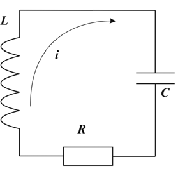
\includegraphics[]{fig/lect5/1a}

                (a)
        \end{minipage}
        \begin{minipage}{0.45\linewidth}
                \centering  
                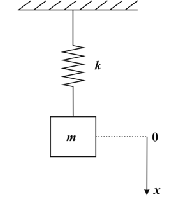
\includegraphics[]{fig/lect5/1b}

                (b)      
        \end{minipage}
        \caption{Линейные осцилляторы: электрический контур (а); груз массы $m$ на пружине с жёсткостью $k$, совершающий малые колебания около положения равновесия (b).}
        \label{fig:5.1}
\end{figure}
т.е. сумма падений напряжения на элементах контура равна нулю, поскольку в цепи отсутствуют внешние источники напряжения. Пусть $i$-- ток, протекающий в контуре, который, как известно, связан с зарядом $q$ следующим образом
\begin{equation}
        \label{eq:5.2}
        i = \dv{q}{t}.
\end{equation}
Тогда для напряжение на элементах контура можно записать
\begin{equation}
        \label{eq:5.3}
        u_R = Ri = R \dv{q}{t}, ~ u_L = L \dv{i}{t} = L \dv[2]{q}{t},~ u_C= \frac{q}{C}.
\end{equation}
Подставляя \eqref{eq:5.3} в \eqref{eq:5.1}, получим уравнение
\begin{equation}
        \label{eq:5.4}
        L\dv[2]{q}{t} + R \dv{q}{t} + \frac{q}{C} = 0.
\end{equation}
Перепишем уравнение \eqref{eq:5.4}, для удобства дальнейшего изложения, в следующем эквивалентном виде
\begin{equation}
        \label{eq:5.5}
        \ddot x + 2 \delta x + \omega_0^2 x =0,
\end{equation}
где 
\begin{equation}
        \label{eq:}
        2 \delta = \frac{R}{L}, ~ \omega_0^2=\frac{1}{LC}.
\end{equation}
Реальные системы, динамика которых описывается уравнением \eqref{eq:5.5}, принято называть
\textbf{линейными осцилляторами}. Уравнение \eqref{eq:5.5} содержит два параметра, имеющих ясный смысл: $\omega_0$--частота собственных колебаний, а параметр $\delta$ характеризует потери в системе.

Другим примером линейного осциллятора может служить груз на пружине (см. рис.\ref{fig:5.1}b), совершающий малые колебания вблизи положения равновесия при наличии силы трения пропорциональной скорости $\dot x$. Динамика такой системы также описывается уравнением \eqref{eq:5.5}, в котором $x$ -- смещение груза из положения равновесия.

\subsection{Гармонический осциллятор}%
\label{sub:5.1.1}

Предположим, что в изолированной физической системе отсутствует
рассеяние энергии, вызванное переходом энергии движения в тепловую
энергию. В таких идеализированных системах запас энергии остаётся
постоянным, и они называются \textbf{консервативными} .

Покажем, что системы, динамика которых описывается уравнением \eqref{eq:5.5}    
при $\delta = 0$, является консервативными, и выясним основные свойства таких
систем. При $\delta = 0$ представим уравнение \eqref{eq:5.5} в виде
\begin{equation}
        \label{eq:5.6}
        \begin{cases}
                \dot x = y, \\
                \dot y = - \omega_0^2 x.
        \end{cases}
\end{equation}
Очевидно, что система \eqref{eq:5.6} имеет единственное состояние равновесия в начале координат, корни характеристического уравнения которого имеют вид: $\lambda_{1,2} = \pm i \omega_0$. Следовательно (см. \ref{lect3}), это состояние равновесия является центом,и на фазовой плоскости $(x,y)$ любая траектория, отличная от состояния
равновесия, представляет собой замкнутую кривую. Уравнение
соответствующих интегральных кривых без труда можно найти из системы
 \eqref{eq:5.6} путём её сведения к уравнению первого порядка с разделяющимися
переменными 
\begin{equation}
        \label{eq:5.7}
        \frac{y^2}{2} + \omega^2 \frac{x^2}{2} = C, C= \const\geq0.
\end{equation}
Из \eqref{eq:5.7} следует, что нетривиальные интегральные кривые системы \eqref{eq:5.6} имеют вид эллипсов, оси которых совпадают с координатными осями. На фазовой плоскости $(x,y)$ согласно первому уравнению
в \eqref{eq:4.6} переменная $x$ вдоль траекторий возрастает при $y>0$ и убывает при $y<0$ (см. рис.\ref{fig:4.2}а). Найдём время $T$, за которое изображающая точка совершит один полный оборот вдоль произвольной замкнутой траектории, стартующей с произвольных начальных условий
\begin{equation}
        \label{eq:5.8}
        x(0) = x_0,~ y(0) = y_0 . 
\end{equation}
Запишем общее решение уравнение \eqref{eq:5.6}
\begin{equation}
        \label{eq:5.9}
        \begin{cases}
                x = C_1 \cos(\omega_o t) + C_2 \sin(\omega_0t), \\
                y = - \omega_0 C_1 \sin(\omega_0t) +\omega_0C_2\cos(\omega_0t),
        \end{cases}
\end{equation}
где $C_{1,2}= \const$. Из \eqref{eq:5.8}, \eqref{eq:5.9} находим уравнение искомой траектории
\begin{equation}
        \label{eq:5.10}
        \begin{cases}
                x=x_0 \cos(\omega_0t) + \frac{y_0}{\omega_0} \sin(\omega_0)
                y = -x_0\omega_0\sin(\omega_0t) + y_0\cos(\omega_0t). 
        \end{cases}
\end{equation}
Очевидно, что в момент $t=T$  должны выполняться условия
\begin{equation}
        \label{eq:5.11}
        x(T) = x_0, ~ y(T)=y_0.
\end{equation}
Подставляя \eqref{eq:5.10} в \eqref{eq:5.11}, получим систему линейных относительно $\sin(\omega_0 T)$ и $\cos(\omega_0t)$ уравнений
 \begin{equation}
        \label{eq:5.12}
        \begin{cases}
                x_0 \cos(\omega_0 T) + \frac{y_0}{\omega_0} \sin(\omega_0 T) = x_0\\
                y_0 \cos(\omega T) - x_0\omega_0 \sin(\omega_0 T) = y_0.
        \end{cases}
\end{equation}

\begin{figure}[h!]
        \centering
        \begin{minipage}{0.45\linewidth}
                \centering  
                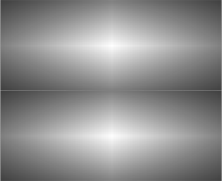
\includegraphics[]{fig/lect5/2a}

                (a)
        \end{minipage}
        \begin{minipage}{0.45\linewidth}
                \centering  
                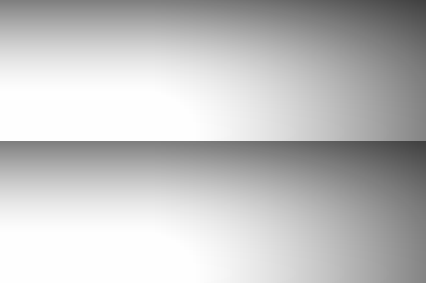
\includegraphics[]{fig/lect5/2b}

                (b)      
        \end{minipage}
        \caption{Фазовый портрет гармонического осциллятора (а); гармонические колебания периода
        $T =  \frac{2\pi}{\omega}~ (b)$.}
        \label{fig:5.2}
\end{figure}
Решая систему \eqref{eq:5.12} обычным образом, находим, что

\begin{equation}
        \label{eq:}
        \cos(\omega_0T) = 1, \quad \sin(\omega_0 T) =0
\end{equation}
следовательно,
\begin{equation}
        \label{eq:5.13}
        T= \frac{2\pi}{\omega_0}.
\end{equation}
Представим для удобства решение \eqref{eq:5.10} в виде
\begin{equation}
        \label{eq:5.14}
        x= A\cos(\omega_0 t+ \phi) \\
        y = -A\omega_0\sin(\omega_0t +\phi),
\end{equation}
где 
\begin{equation}
        \label{eq:}
        A= \sqrt{ x_0^2 + \frac{y_0^2}{\omega_0^2}}, \quad \tg{ \phi} = \frac{\omega_0x_0}{y_0}.
\end{equation}
Из \eqref{eq:5.13}, \eqref{eq:5.14} вытекает, что осциллятор \eqref{eq:5.9} при любых начальных условиях
совершает \textbf{ синусоидальные (гармонические) } колебания с амплитудой $A$, фазой $\phi$ и частотой $\omega_0$, независящей от начальных условий (см. рис.\ref{fig:5.2}b). Осциллятор \eqref{eq:5.6} называется гармоническими, а совершаемые им колебания, период которых не зависит от начальных условий, -- \textbf{ изохронными}.
При этом уравнение \eqref{eq:5.7} представляет собой закон сохранения энергии, поскольку первое слагаемое в \eqref{eq:5.7} есть кинетическая

\begin{equation}
        \label{eq:5.15}
        E_K = \frac{y^2}{2} = (A^2 \omega_0^2 \cos^2(\frac{\omega_0 t + \phi)}{2},
\end{equation}
а второе -- потенциальная энергия осциллятора
\begin{equation}
        \label{eq:5.16}
        E_{\text{П}} = \frac{x^2}{2} = (A^2 \omega_0^2 \sin^2(\frac{\omega_0t + \phi)}{2}.
\end{equation}
Из \eqref{eq:5.7}, \eqref{eq:5.15} и \eqref{eq:5.16} следует, что полная энергия осциллятора остаётся при колебаниях постоянной
\begin{equation}
        \label{eq:}
        E = E_K + E_{\text{П}} = \const,
\end{equation}
однако переходит из одного вида в другой.

Поясним теперь связь между траекториями на фазовой плоскости осциллятора \eqref{eq:4.6} и колебаниями в реальном пространстве. Это соотношение иллюстрирует рис.\ref{fig:5.3}, на котором представлена замкнутая фазовая траектория осциллятора \eqref{eq:5.6}, описывающего малые колебания груза на пружине (рис.\ref{fig:5.1}b), и четыре состояния груза в пространстве, соответствующие различным точкам фазовой траектории. 
\begin{figure}[h!]
        \centering
        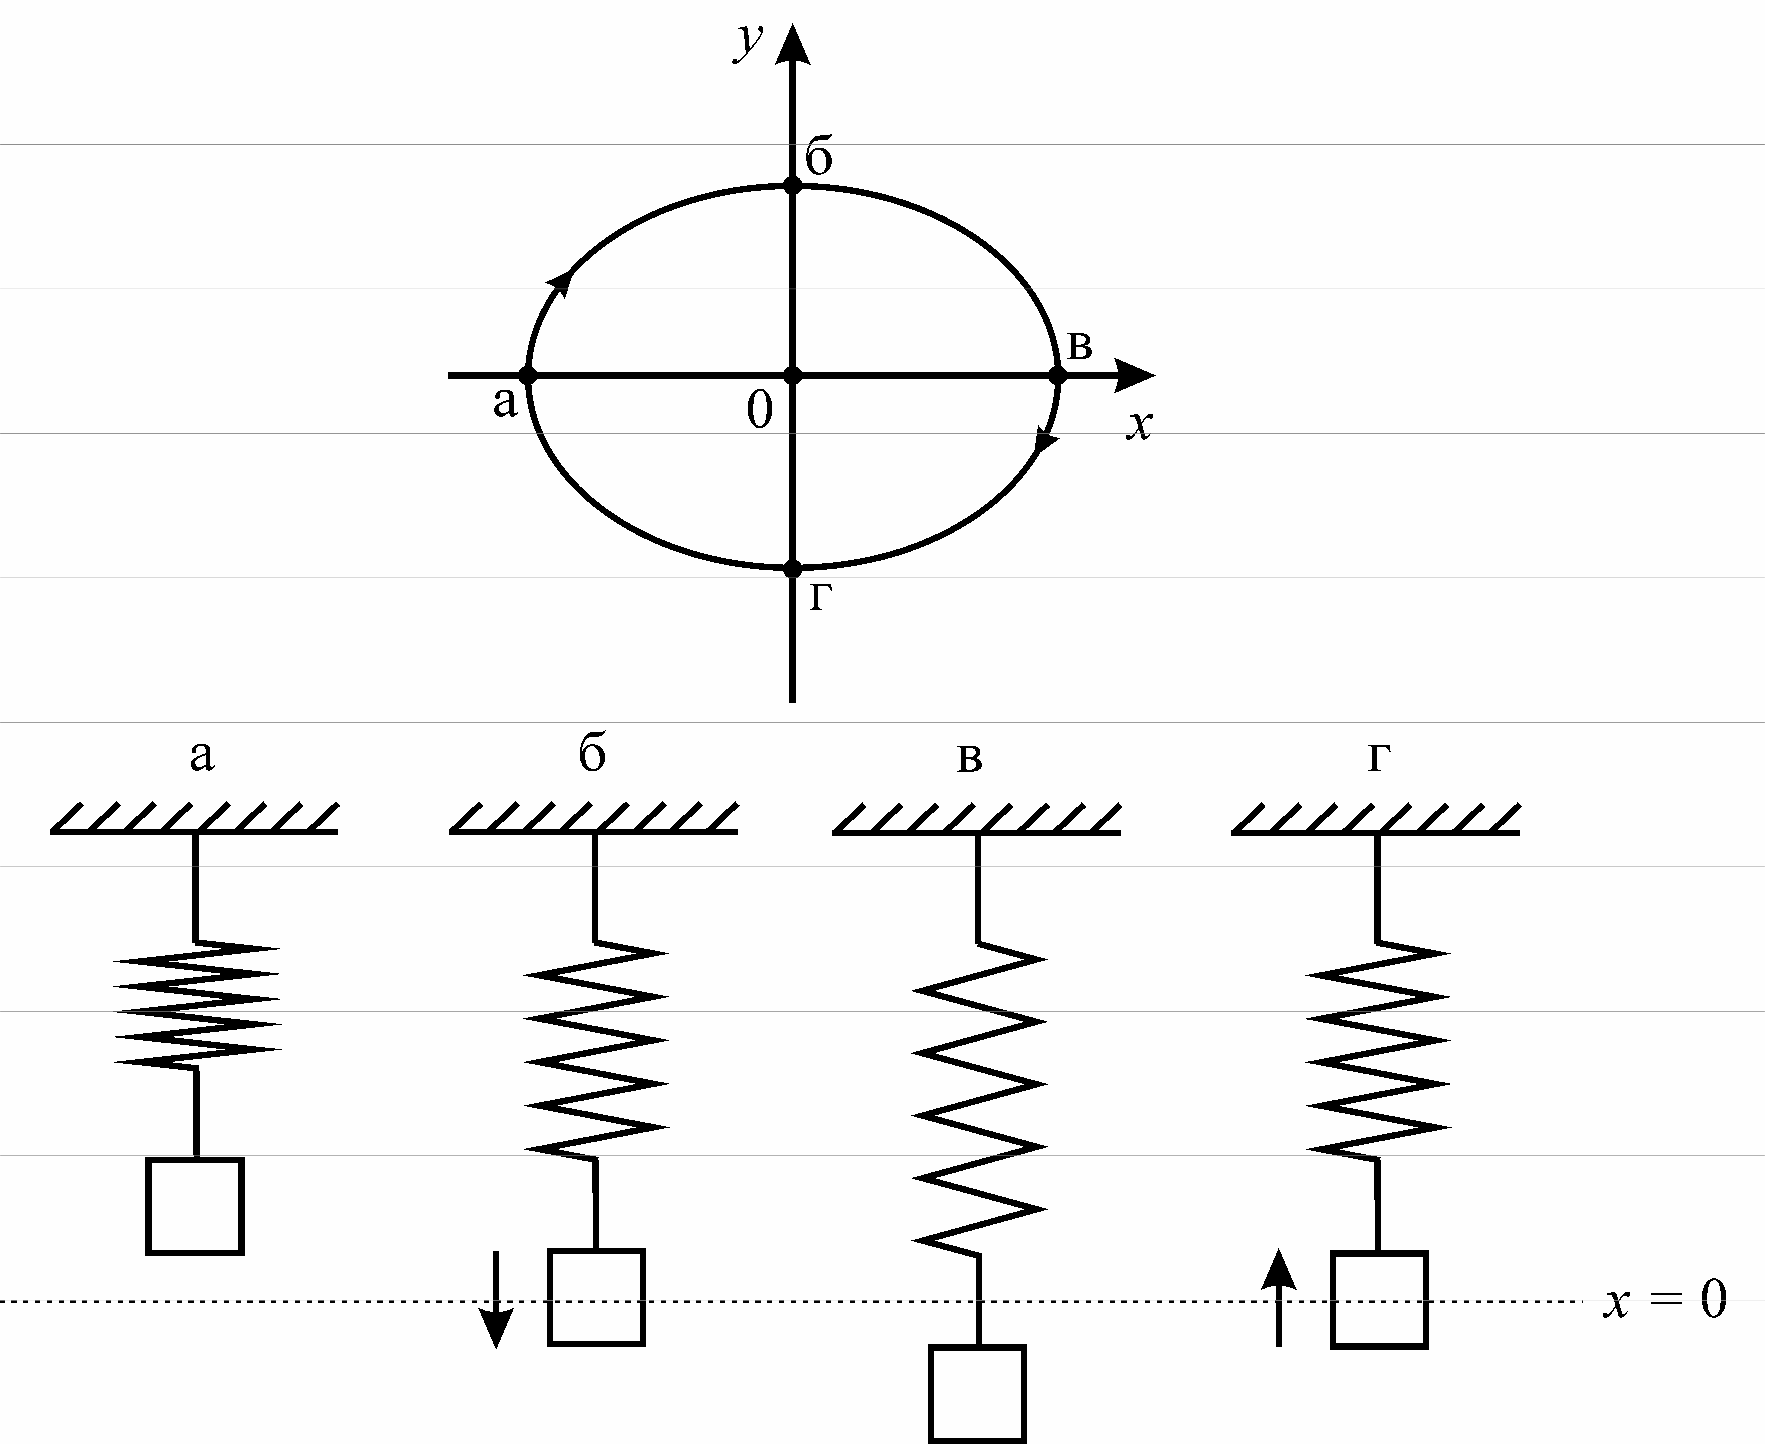
\includegraphics[width=0.6\linewidth]{fig/lect5/3}
        \caption{Фазовая траектория осциллятора \eqref{eq:5.6} и четыре различных состояния груза на пружине  }
        \label{fig:5.3}
\end{figure}


\subsection{Линейный осциллятор при наличии потерь}%
\label{sub:5.1.2}

В реальных системах всегда происходит рассеяние (диссипация) энергии,
её потери, вызванные наличием элементов, трансформирующих энергию
движения в тепловую. Например, в электрическом контуре это омическое
сопротивление, а в случае груза на пружине – сила трения (рис.\ref{fig:5.1}). Если
диссипация энергии в системе (линейной или нелинейной) ничем не
компенсируется, то с течением времени любые колебания затухают и система
приходит в равновесное состояние. Такие системы называют диссипативными
динамическими системами (см. лекцию \ref{lect1}), и их динамика принципиально
отличается от динамики консервативных систем.

Рассмотрим динамику простейшей диссипативной системы -- линейного осциллятора \eqref{eq:5.5} при $\delta \neq 0$. Перепишем \eqref{eq:5.5} в виде системы
\begin{equation}
        \label{eq:5.17}
        \dot x = y, \\
        \dot y = -2 \delta y - \omega_0^2 x.
\end{equation}
На фазовой плоскости $(x,y)$ система \eqref{eq:5.17} имеет единственное состояние равновесия $O(x=0,y=0)$, характеристическое уравнение для которого имеет вид
\begin{equation}
        \label{eq:5.18}
        \lambda^2 + 2 \delta \lambda + \omega_0^2 = 0 
\end{equation}
Динамика двумерных линейных систем полностью определяются типом состояний равновесия (см. лекцию 
\ref{lect3}). Поэтому, анализируя корни уравнения \eqref{eq:5.18}, можно установить возможные колебательные процессы в линейном осцилляторе \eqref{eq:5.17}.

\paragraph{Затухающий процесс.}%
\label{par:zatukhaiushchii_protsess_}

Пусть параметры системы \eqref{eq:5.17} удовлетворяют условиям
\begin{equation}
        \label{eq:5.19}
        \delta > 0, \delta^2 < \omega_0^2.
\end{equation}
Поскольку $\Re \lambda_{1,2} = - \delta < 0 $ состояние равновесия $O$ является устойчивым фокусом
(см. лекцию \ref{lect3}, траекториям которого отвечают осцилляторно затухающие колебания. Фазовый портрет систем \eqref{eq:5.17} представлен на рис.\ref{fig:5.4}а. Траектории пересекают ось абсцисс так, что касательные к ним в точках пересечения имеют вертикальный наклон, поскольку $\dot x =0$, если $y=0$. Кроме того,
\begin{equation}
        \label{eq:}
        \dot y =0, \text{ если } y= - \frac{\omega_0^2}{2\delta}x
\end{equation}
и, следовательно, траектории пересекают эту прямую так, что в точках пересечение наклон касательных к траекториям является горизонтальным. Линии на фазовой плоскости, на которых касательные к траекториям имеют один и тот же наклон называют
\textbf{изоклинами}
соответствующего наклона. В случае системы \eqref{eq:5.17} ось абцисс -- изоклина вертикальных, а прямая $y = - \frac{\omega_0^2}{2\delta}x$-- горизонтальных наклонов.

Исследуем характеристики осцилляторно затухающего процесса. Аналогично \eqref{eq:5.10}, запишем уравнение траектории осциллятора \eqref{eq:5.17}, удовлетворяющей начальным условиям $x(0) = x_0, y(0) = y_0$ 
\begin{equation}
        \label{eq:5.21}
        \begin{cases}
                x=e^{-\delta t} \qty[ x_0 \cos( \omega t) + \frac{y_0- \delta x_0}{\omega} \sin(\omega t) ] ,\\
                y= e^{-\delta t} \qty[\cos(\omega t) - \frac{( -\omega^2 + \delta^2) x_0 + \delta y_0}{\omega} \sin(\omega t)],
        \end{cases}
\end{equation}
или
\begin{equation}
        \label{eq:5.22}
        \begin{cases}
                x = A e^{-\delta t} \sin(\omega t + \phi),\\
                y = i \sqrt{ \delta^2 + \omega^2} A e^{-\delta t} \sin(\omega t + \phi +  \theta),
        \end{cases}
\end{equation}
где 
\begin{equation}
        \label{eq:}
        A = \sqrt{ x_0^2 + \frac{( y_0 + \delta x_0)^2}{\omega^2}}, ~ \tg \phi = \frac{x_0 \omega}{y_0 + \delta x_0}, ~ \tg \theta = - \frac{\omega}{\delta}.
\end{equation}
Из \eqref{eq:5.22} следует, что колебательные процессы, описываемые системой \eqref{eq:5.17} при выполнении условий \eqref{eq:5.19}, являются непериодическими и осцилляторно затухающими. Затухание колебаний происходит по экспоненциальному закону, т.е. на плоскости $(t,x)$ экстремумы функции $x(t)$ лежат на экспонентах $x= \pm A e^{-\delta t}$ (см. рис.\ref{fig:5.3}b). Интервал между любыми двумя соседними экстремумами равен $T = \frac{ 2 \pi}{\omega}$.
Благодаря этому свойству, можно ввести величину, характеризующую скорость затухания осцилляторного процесса -- логарифмический декремент затухания $d$. Пусть $x_1(t_1)$ и $x_2(t_2), t_2>t_1$ -- значение двух соседних экстремумов, например максимумов, т.е.
\begin{equation}
        \label{eq:}
        x_1(t_1) = A e^{- \delta t_2}, \quad x_2(t_2) = A e^{-\delta t_2}.
\end{equation}
Найдем их отношение
\begin{equation}
        \label{eq:5.23}
        \frac{x_1(t_1)}{x_2(t_2)} = e ^{\delta(t_2-t_1)} = e^{\delta T} = e^{\frac{\delta2 \pi}{\omega}}.
\end{equation}
Декремент характеризует убывание амплитуды колебаний во времени, т.е. число $\frac{1}{d}$ равно числу колебаний, после которого амплитуда уменьшится в $e $ раз. Заметим, что этот закон затухания колебания выполняется во-первых, если система является линейной, а во-вторых, если потери энергии происходят линейно относительно $\dot x$. Нарушение этих условий делает соотношение \eqref{eq:5.23}не справедливым и использование декремента для характеристики  процесса требует специальных оговорок.

\begin{figure}[h]
        \centering
        \begin{minipage}{0.45\linewidth}
                \centering  
                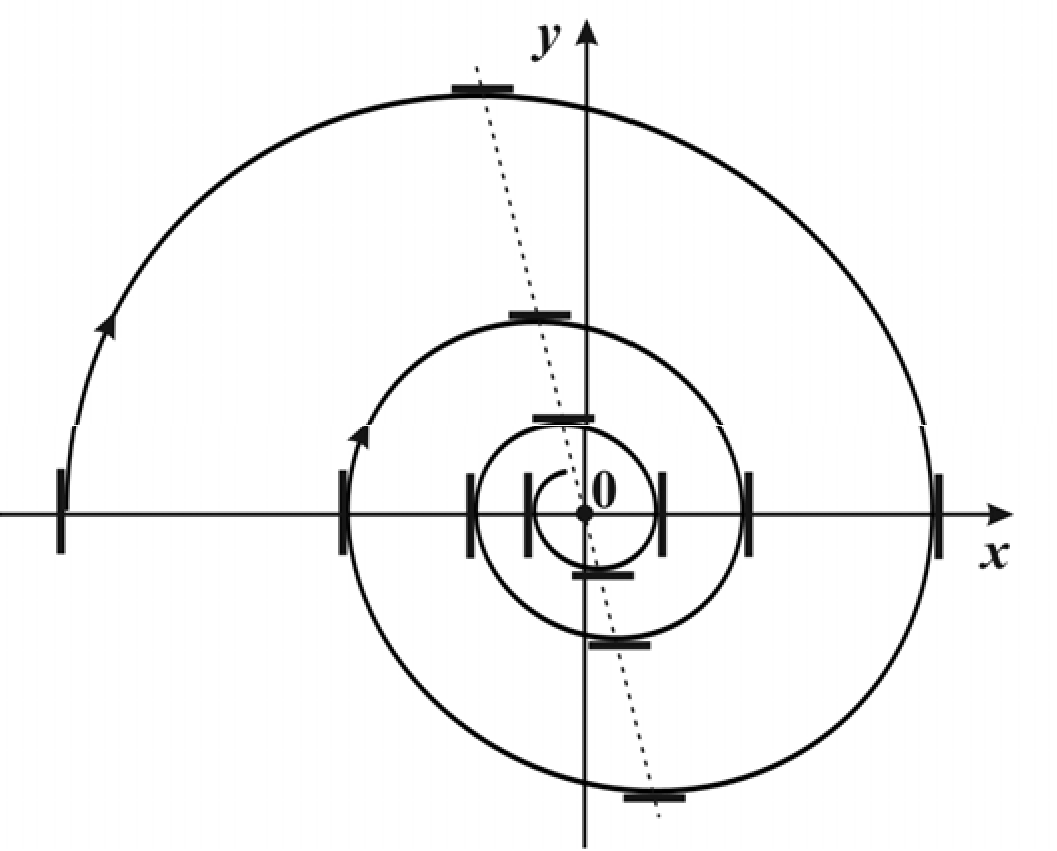
\includegraphics[]{fig/lect5/4a}

                (a)
        \end{minipage}
        \begin{minipage}{0.45\linewidth}
                \centering  
                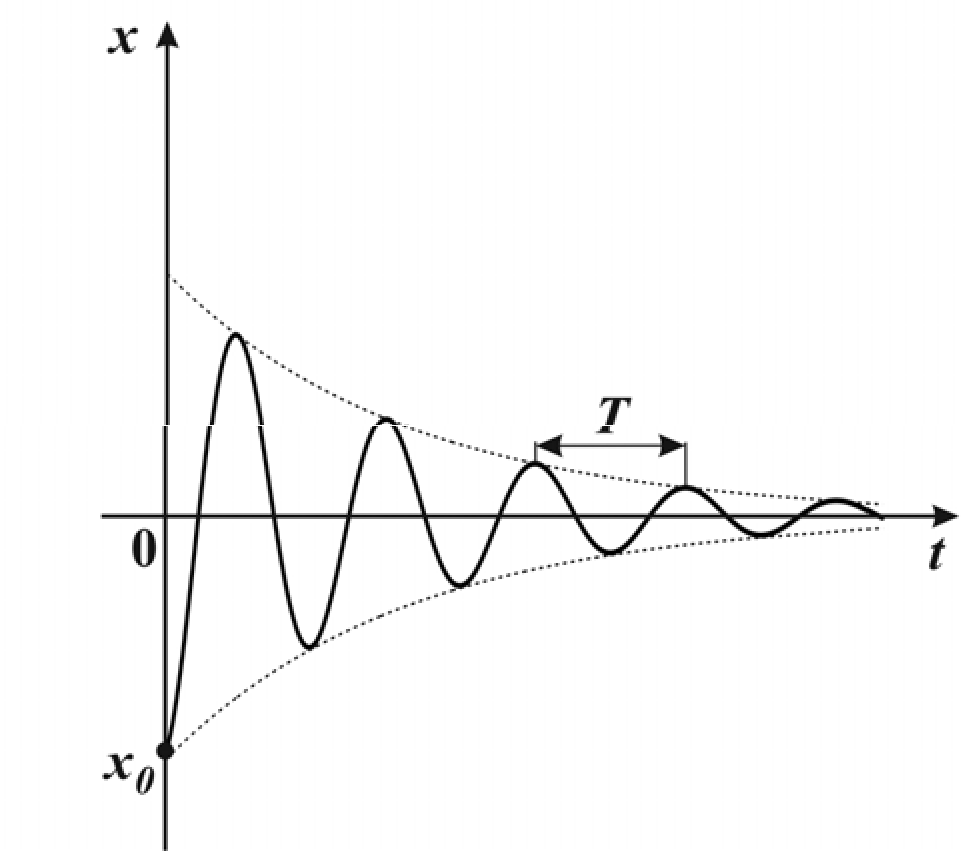
\includegraphics[]{fig/lect5/4b}

                (b)      
        \end{minipage}
        \caption{Устойчивый фокус, пунктирной линией показана изоклина горизонтальных наклонов (а); осцилляторно затухающие колебания (b). }
        \label{fig:5.4}
\end{figure}



\paragraph{Затухающий апериодический процесс.}%
\label{par:zatukhaiushchii_aperiodicheskii_protsess_}

Предположим, что параметры системы \eqref{eq:5.17} удовлетворяют условиям
\begin{equation}
        \label{eq:5.24}
        \delta>0,~ \delta^2 > \omega_0^2
\end{equation}
При выполнении \eqref{eq:5.24} состояние равновесия $O$ имеет отрицательные корни характеристического уравнения
\begin{equation}
        \label{eq:5.25}
        \lambda_{1,2} = - \delta \pm \sqrt{ \delta^2 - \omega_0^2}
\end{equation}
и, следовательно, является устойчивым узлом (см. рис.\ref{fig:5.5}а) каждой траекторий которого отвечает затухающий апериодический процесс осциллятора. Несмотря на то, что при всех начальных условиях наблюдается однотипное поведение осциллятора, некоторая, не принципиальная, разница в характере установления равновесного состояния всё-таки существует. Эта разница определяется расположением начальных условий на фазовой плоскости относительно 
ведущего и неведущих направлений узла (см. лекцию \ref{lect3}). Для узла $O$ эти направления задаются соответственно уравнениями
\begin{equation}
        \label{eq:5.26}
        y= \lambda_1 x, ~ y=\lambda_2 x.
\end{equation}
Прямые \eqref{eq:5.26} делят фазовуб плоскость на четыре области (см. рис.\ref{fig:5.5}а). Для начальных условий из областей 2, 4 апериодически затухающие процессы характеризуются монотонным изменением переменных $x(t)$, $y(t)$, а из области 1, 3 -- наличием экстремумов в моменты времени, когда траектории пересекают ось абсцисс (см. рис.\ref{fig:5.5}). 
\begin{figure}[h]
        \centering
        \begin{minipage}{0.45\linewidth}
                \centering  
                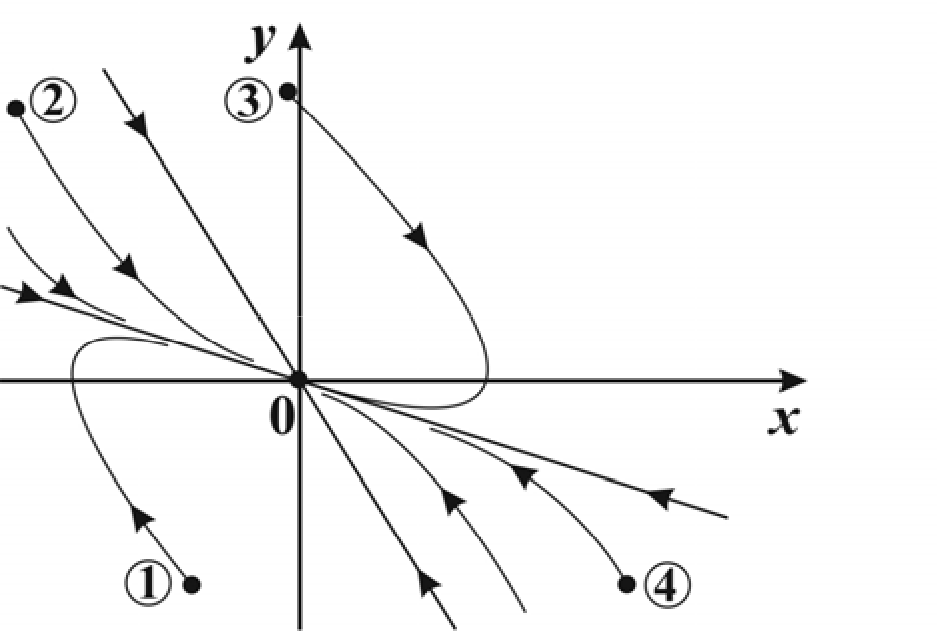
\includegraphics[]{fig/lect5/5a}

                (a)
        \end{minipage}
        \begin{minipage}{0.45\linewidth}
                \centering  
                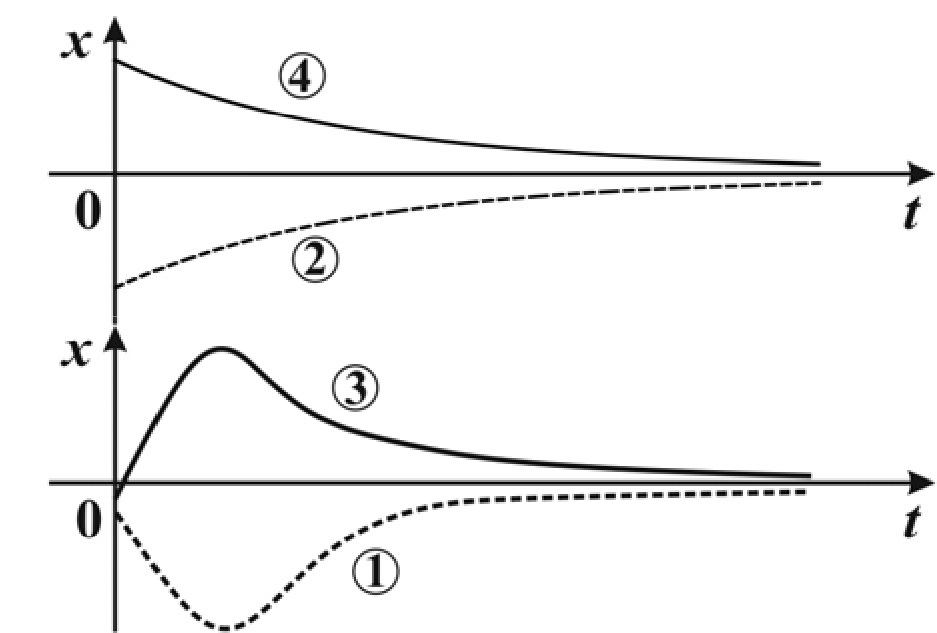
\includegraphics[]{fig/lect5/5b}

                (b)      
        \end{minipage}
        \caption{Устойчивый узел (а); апериодические затухающие процессы, соответствующие начальным условиям из области 1-4 (b).}
        \label{fig:5.5}
\end{figure}

\subsection{Линейный осциллятор с <<отрицательным>> затуханием}%
\label{sub:5.1.3}

Пусть в системе \eqref{eq:5.17} теперь параметр $\delta<0$. Рассмотрим изменение во времени полной энергии осциллятора, задаваемой уравнениями \eqref{eq:5.15}, \eqref{eq:5.16}. В силу системы \eqref{eq:5.17} имеем
\begin{equation}
        \label{eq:5.27}
        \pdv{E}{t} = y \dot y + \omega_0^2 x \dot x = - 2\delta y^2
\end{equation}
Поскольку $\delta<0$ из \eqref{eq:5.27} следует, что энергия $E$ во времени растёт. Понятно, что для этого осциллятор должен пополнять энергию из вне, так как собственного источника энергии у него нет. В некоторых системах (так называемых активных) за счёт внешних источников энергии возможно формирование таких динамических процессов с <<отрицательным>> затуханием (трением) или <<отрицательным>> сопротивлением, приводящих к временному росту энергии.
Примерами подобных систем являются: в радиоэлектронике -- устройства,
содержащие элементы, у которых вольт-амперные характеристики имеют
падающие участки, в механике --  системы, в которых силы трения имеют
нелинейную, с падающим участком, зависимость от относительной скорости
трущихся поверхностей (например, маятники на вращающихся валах) и др.
Динамика таких систем в окрестности равновесных состояний приближённо
может быть описана с помощью системы \eqref{eq:5.17} при $\delta<0$.

Рассмотрим динамику системы \eqref{eq:5.17} при $\delta<0$. В этом случае из \eqref{eq:5.20} и \eqref{eq:5.25} следует, что состояние равновесия является неустойчивым фокусом если $\delta^2<\omega_0^2$ (см. рис.\ref{fig:5.6}а) или неустойчивым узлом, если $\delta^2 \geq \omega_0^2$ (см. рис.\ref{fig:5.6}b). Следовательно, при $\delta<0$ осциллятор \eqref{eq:5.27} описывает нарастающие колебания,
примеры которых даны на рис.\ref{fig:5.6}c и рис.\ref{fig:5.6}d. 
\begin{figure}[h]
        \centering
        \begin{minipage}{0.45\linewidth}
                \centering  
                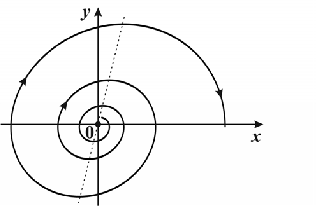
\includegraphics[]{fig/lect5/6a}

                (a)
        \end{minipage}
        \hfill
        \begin{minipage}{0.45\linewidth}
                \centering  
                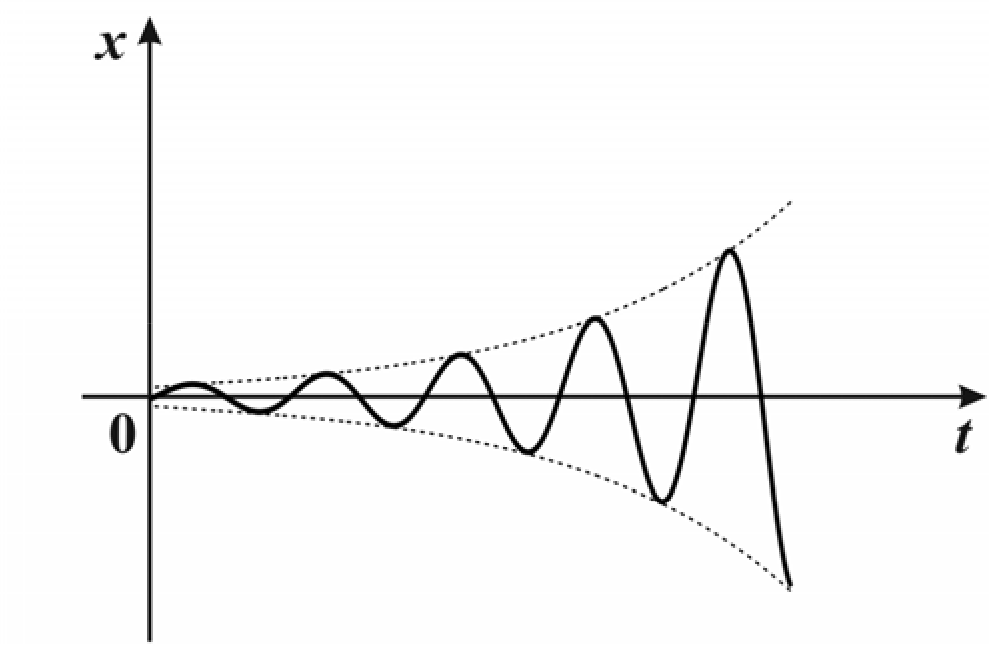
\includegraphics[]{fig/lect5/6b}

                (b)      
        \end{minipage}
        \vfill
        \begin{minipage}{0.45\linewidth}
                \centering  
                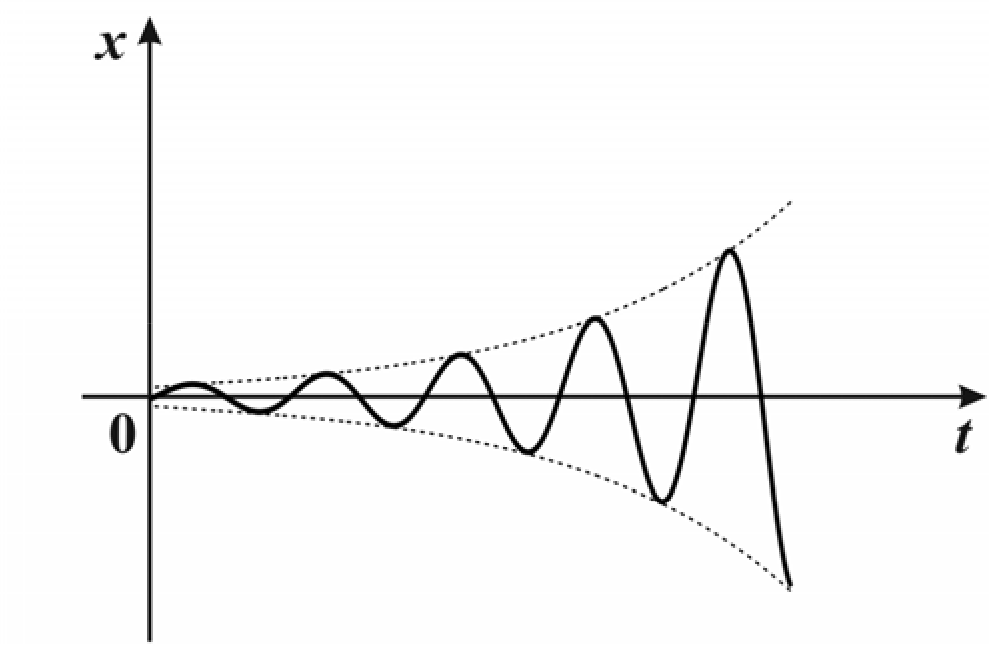
\includegraphics[]{fig/lect5/6c}

                (c)
        \end{minipage}
        \hfill
        \begin{minipage}{0.45\linewidth}
                \centering  
                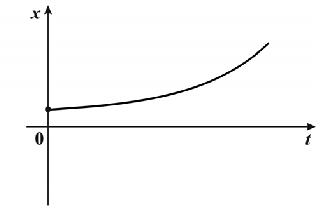
\includegraphics[]{fig/lect5/6d}

                (d)      
        \end{minipage}
        \caption{Неустойчивый фокус (а); неустойчивый узел (b); осцилляторно нарастающий процесс (c); апериодический нарастающий процесс (d).}
        \label{fig:5.6}
\end{figure}
В случае фокуса колебание
нарастают по экспоненциальному закону (рис. \ref{fig:5.6}c), который характеризуется
так называемым логарифмическим \textbf{инкрементом нарастания}
$\delta_1= -\delta$,
применяемым без оговорок лишь для линейных систем. В случае узла вид
нарастающих колебаний зависит от позиции на фазовой плоскости начальных
условий относительно ведущего и неведущего направлений, т.е. может
происходить как монотонно (\ref{fig:5.6}c), так и не монотонно (с одним
экстремумом) во времени.

Таким образом, <<отрицательное>> трение (потери) приводят к
неограниченному росту колебаний, что, конечно, не может происходить в
реальных системах. Этот рост является следствием линейной идеализации
задачи и, как мы увидим в дальнейшем, нелинейные механизмы его
ограничивают.

\section{Динамика нелинейного осциллятора}%
\label{sec:5.2}

Как мы уже отмечали, линейные системы представляют собой
простейшие, идеализированные модели реальных процессов. Даже сильно
упрощённые модели реальных систем, как правило, являются нелинейными.
Например, незначительное изменение условий задач, рассмотренных в разделе
\ref{sec:5.1}, приводит к модели в виде уже нелинейного осциллятора. Так, если в задаче
о колебаниях груза (рис.\ref{fig:5.1}b) не ограничиваться малыми смещениями, то сила с
которой пружина действует на груз будет нелинейной функцией смещения и
осциллятор становится нелинейным. Другим примером нелинейного
осциллятора может служить электрический контур, представленный на
рис.\ref{fig:5.1}а, в случае, если ёмкость $C$ содержит сегнетоэлектрик.
\subsection{Консервативный нелинейный осциллятор}%
\label{sub:5.2.1}

Предположим, что рассеяние энергии в реальной системе происходит
очень медленно – например, груз на пружине помещён в среду с очень малым
трением, в электрическом контуре отсутствует сопротивление $R$, а омическое
сопротивление соединительных проводов пренебрежимо мало и так далее.
Ясно, что этом случае диссипативные механизмы, обеспечивающие рассеяние
энергии, не окажут сильного влияния (на не слишком больших временных
интервалах) на динамику системы и ими можно пренебречь. Другими словами,
можно считать, что в этом случае система является консервативной. Основной
моделью таких систем является консервативный осциллятор, динамика
которого описывается уравнением
\begin{equation}
        \label{eq:5.28}
        \ddot x + f(x) = 0,
\end{equation}
где $f(x)$ -- нелинейная функция. В частности, к уравнению вида \eqref{eq:5.28} могут быть сведены упомянутые выше осцилляторы. Представим для удобства уравнения \eqref{eq:5.28} в виде системы
\begin{equation}
        \label{eq:5.29}
        \begin{cases}
                \dot x = y, \\
                \dot y = -f(x).
        \end{cases}
\end{equation}
Прежде всего, покажем, что динамика системы \eqref{eq:5.29} является консервативной. Поделив второе уравнение системы \eqref{eq:5.29} на первое и разделив переменные, имеем
\begin{equation}
        \label{eq:5.30}
        y \dd{y} = - f(x) \dd{x}.
\end{equation}
Проинтегрируем уравнение \eqref{eq:5.30} от некоторого начального момента $t=t_0$ до произвольного момента времени $t$. В результате получим
\begin{equation}
        \label{eq:5.31}
        \frac{y^2}{2} - \frac{y_0^2}{2} = - \int\limits_{x_0}^{x} f(x) \dd{x}, 
\end{equation}
где $x_0 = x(t_0),~ y_0=y(t_0)$. Нетрудно видеть, что уравнение \eqref{eq:5.31} можно переписать в следующем виде
\begin{equation}
        \label{eq:5.32}
        \frac{y^2}{2} + \int\limits_{0}^{x_0} f(x) \dd{x} = h, 
\end{equation}
где
\begin{equation}
        \label{eq:5.33}
        h=\frac{y_0^2}{2} + \int\limits_{0}^{x_0}  f(x) \dd{x}.
\end{equation}
Из \eqref{eq:5.33} следует, что $h = \const$ и представляет собой полную энергию осциллятора \eqref{eq:5.29} в момент $t= t_0$. В левой же части уравнения \eqref{eq:5.32} стоит полная энергия осциллятора в момент $t$, состоящая из суммы
кинетической $E_K$  потенциальной $E_{\text{П}}$ энергии, где
\begin{equation}
        \label{eq:5.34}
        E_K = \frac{y^2}{2}, \quad E_{\text{П}} = \int\limits_{0}^{x} f(x) \dd{x}. 
\end{equation}
Таким образом, с одной стороны уравнение \eqref{eq:5.32} задаёт закон сохранения энергии, а с другой -- в неявном виде уравнение интегральных кривых, отвечающих данному $h$. Заметим, что, если для данного $h$ из \eqref{eq:5.32} найти действительных значений $(x,y)$ не удаётся, то это означает, что энергия осциллятора \eqref{eq:5.29} не может принимать такого значения.

Покажем теперь как, используя уравнение \eqref{eq:5.32}, можно построить фазовый портрет системы \eqref{eq:5.29}.

Предварительно приведём некоторые свойства траекторий, вытекающие непосредственно из системы \eqref{eq:5.29} и уравнения \eqref{eq:5.32}. Из \eqref{eq:5.29} следует, что координаты состояний равновесия этой системы определяются системой
\begin{equation}
        \label{eq:5.35}
        y=0, \quad f(x)=0
\end{equation}
и, следовательно, они расположены на оси абсцисс. При этом, так как $\dot x = 0$ при $y=0$ во всех точках оси абсцисс, отличных от состояний равновесия, касательные к траекториям имеют вертикальный наклон, то есть ось абсцисс на этих участках является изоклиной вертикальных наклонов. Кроме того, поскольку уравнение \eqref{eq:5.32} инвариантно относительно замены $y \to -y$, то фазовые траектории системы \eqref{eq:5.29} симметричны относительно оси абсцисс. 
Поэтому достаточно установить вид траекторий лишь на верхней полуплоскости, а поведение траекторий при $y<0$
 можно найти, используя свойство симметрии.

 Рассмотрим теперь процедуру построения фазового портрета системы \eqref{eq:5.29} с помощью уравнения \eqref{eq:5.32}. Из \eqref{eq:5.34} вытекает, что
 \begin{equation}
         \label{eq:5.36}
         \pdv{E_{\text{П}}}{x} = f(x)
 \end{equation}
 Следовательно, в состояниях равновесия потенциальная энергия $E_{\text{П}}(x)$ либо достигает экстремума, либо имеет точку перегиба. Проанализируем поведение фазовых траекторий системы
 \eqref{eq:5.29} в окрестности состояний равновесия, соответствующих этим трём случаям. Для этого из \eqref{eq:5.32} выразим $y$ через $E_{\text{П}}(x)$ 
 \begin{equation}
         \label{eq:5.37}
         y = \sqrt{ 2 \qty[ h - E_{\text{П}}(x)] }
 \end{equation}
 Согласно \eqref{eq:5.37} траектории системы \eqref{eq:5.29} соответствующие данному $h$, существуют на фазовой плоскости только для тех $x$, где $E_{\text{П}}(x) \leq h$. Причём, для
 $x$, удовлетворяющих уравнению $E_{\text{П}} = h$ и переменная $y=0$. В силу \eqref{eq:5.37} имеем 
 \begin{equation}
         \label{eq:5.38}
         \dv{y}{x} = - \frac{  \dv{ E_{ \text{П} } } {x}  } 
         {\sqrt{2 \qty[ h - E_{\text{П}}(x) ] }}
 \end{equation}
 Отсюда получаем, ещё одно свойство траекторной системы \eqref{eq:5.29}
 \begin{equation}
         \label{eq:5.39}
         \begin{cases}
                 \dv{y}{x} > 0, & \text{ если } \dv{E_{\text{П} } }{x} < 0, \\
                 \dv{y}{x} < 0, & \text{ если } \dv{E_{\text{П} } }{x} > 0. \\
         \end{cases}
 \end{equation}
 Опираясь на представленные здесь свойства траекторий, можно построить фазовый портрет системы \eqref{eq:5.29}, зная лишь вид функции $E_{\text{П}}(x)$. Рис. \ref{fig:5.7} иллюстрирует методику такого построения в случае, когда $E_{\text{П}}(x)$ имеет локальные минимум, максимум и точку перегиба. Если функция $E_{\text{П}}(x)$ имеет минимум, то на фазовой плоскости система \eqref{eq:5.29} имеет состояние равновесия типа центр (см. рис.\ref{fig:5.7}а), которое устойчиво по Ляпунову. Максимум функции
 $E_{\text{П}}(x)$ соответствует на фазовой плоскости седло (см. рис.\ref{fig:5.7}b). Заметим, что в силу \eqref{eq:5.37} у седла нелинейной системы \eqref{eq:5.29} сепаратрисы имеют вид некоторых кривых, а не прямых, как в случае линейного осциллятора.
 Наконец, если $E_{\text{П}}(x)$ имеет точку перегиба, то на фазовой плоскости существует сложное состояние равновесия (см. рис.\ref{fig:5.7}c), имеющие два нулевых корня характеристического уравнения.

 Изложенный выше приём построения фазового портрета осциллятора \eqref{eq:5.29} справедлив не только для анализа поведение траекторий в окрестности состояний равновесия, но и для построения полного фазового портрета на всей фазовой плоскости. Продемонстрируем это на примере нелинейного осциллятора, описывающего колебание математического маятника.

 Рассмотрим динамику маятника, состоящего из невесомого стержня длины $l$ и груза массы $m$ (см. рис.\ref{fig:5.8}а). Маятник находится в поле силы тяжести и может свободно вращаться в вертикальной плоскости вокруг точки подвеса.

 \begin{figure}[h]
         \centering
         \includegraphics[width=0.6\linewidth]{example-image-a}
         \caption{Три различных вида функции $E_{\text{П}}(x)$ и отвечающие им фазовые портреты системы \eqref{eq:5.29}: состояние равновесия (а); состояние равновесия седло (b); сложное состояние равновесия с двумя нулевыми характеристическими корнями (c).}
         \label{fig:5.7}
 \end{figure}

 Пусть $\phi$ -- угол отклонения маятника от вертикали. Запишем уравнение движения маятника
 \begin{equation}
         \label{eq:5.40}
         J \dv{\omega}{t} = \sum\limits_{k} M_k,
 \end{equation}
 где $J$--момент инерции груза, $J= ml^2$, $\omega = \dv{\phi}{t}$-- угловая скорость массы $m$, $M_k$-- момент сил, действующих на груз. На груз действует две силы -- тяжести и вязкого трения, которая пропорциональна мгновенной скорости и равна -- $k l \dot \phi$, $k>0$. Моменты этих сил будем вычислять относительно оси, проходящей через точку подвеса маятника перпендикулярно плоскости колебаний маятника. Они определяются следующим образом
 \begin{equation}
         \label{eq:5.41}
         M_1 = - mgl \sin \phi, \quad M_2 = - kl^2 \pdv{\phi}{t},
 \end{equation}
 где $g$ -- ускорение свободного падения. Подставляя \eqref{eq:5.41} в \eqref{eq:5.40}, получим
 \begin{equation}
         \label{eq:5.42}
         ml^2 \dv[2]{\phi}{t} = - mgl\sin \phi - kl^2 \dv{\phi}{t}.
 \end{equation}
 \begin{figure}[h]
         \centering
         \includegraphics[width=0.6\linewidth]{example-image-a}
         \caption{Колебательные движения маятника (а), вращательные движения маятника (b); 
         потенциальная функция (c); фазовый портрет осциллятора \eqref{eq:5.43} (d).}
         \label{fig:5.8}
 \end{figure}
 Сделаем в \eqref{eq:5.42} замену времени $t = \sqrt{ \frac{l}{g}} \tau$, в результате которой это уравнение примет вид
 \begin{equation}
         \label{eq:5.43}
         \ddot \phi + \lambda \dot \phi + \sin \phi =0,
 \end{equation}
 где точкой обозначено дифференцирование по $\tau$, а $\lambda = \frac{k}{m} \sqrt{ \frac{l}{g}}$
-- безразмерный параметр, характеризующий диссипативные потери в системе.

Исследуем сначала динамику уравнения \eqref{eq:5.43} в случае отсутствия диссипативных потерь, т.е. в случае $\lambda=0$. При $\lambda=0$ уравнение \eqref{eq:5.43} эквивалентно системе
\begin{equation}
        \label{eq:5.44}
        \begin{cases}
                \dot \phi = y, \\
                \dot y = - \sin \phi.
        \end{cases}
\end{equation}
В силу периодичности по $\phi$ правой части системы \eqref{eq:5.44} её фазовым пространством является цилиндр $G = S^1 \times \R$. Цилиндричность фазового пространства системы \eqref{eq:5.44} имеет ясный физический смысл -- маятник может совершать движения как без вращения (см. рис.\ref{fig:5.8}а),
так и с вращением вокруш точка подвеса (см. рис.\ref{fig:5.8}b). Для построения фазового портрета осциллятора \eqref{eq:5.44} воспользуемся методикой изложенной выше. Рассмотрим потенциальную энергию осциллятора \eqref{eq:5.44} -- $E_{\text{П}}(\phi) = - \cos \phi$. Построив график функции $E_{\text{П}}(x)$ (см. рис.\ref{fig:5.8}c) и расположим под ним развёртку фазового цилиндра, мы без труда получаем
фазовый портрет осциллятора \eqref{eq:5.44} (см. рис.\ref{fig:5.8}d). На цилиндрической фазовой поверхности существуют два состояния равновесия: центр -- $O_1(0,0)$ и седло -- $O_1(\pi,0)$. Сепаратрисы седла делят все остальные нетривиальные траектории на два различных 
континуальных семейства периодических
траекторий. К первому семейству относятся периодические траектории из
области ограниченной сепаратрисами. Эти траектории не охватывают фазовый
цилиндр и определяют колебательные движения маятника, т.е. движения без
проворотов вокруг оси подвеса (рис.\ref{fig:5.8}а). Второе семейство образуют
периодические траектории, охватывающие фазовый цилиндр и отвечающие
вращательным движениям маятника (рис.\ref{fig:5.8}b).

Перейдём к обсуждению свойств колебательных процессов осциллятора
\eqref{eq:5.44}. Заметим, что система \eqref{eq:5.44} легко сводится к одному уравнению с
разделяющимися переменными, которое можно проинтегрировать и получить
точные решения, дающие полную информацию о свойствах колебательных
процессов. Такой путь требует привлечения теории эллиптических интегралов
и эллиптических функций Якоби. Мы поступим по-другому – приведём здесь
лишь качественные рассуждения, основанные на свойствах фазовых
траекторий, которые позволяют, тем не менее, установить основные свойства
колебательных процессов.

Рассмотрим сначала колебательные движения осциллятора, которые
существуют, если начальная энергия $h \in (-1,1)$. Для траекторий, локализованных
в малой окрестности состояния равновесия $O_1$ (начальная энергия близка к
значению $-1$), можно считать в первом приближении, что $\sin \phi \simeq \phi$ и колебания
осциллятора \eqref{eq:5.44} близки к колебаниям линейного осциллятора.
Следовательно, малые (вблизи дна потенциальной ямы) колебания осциллятора
\eqref{eq:5.44} будут периодическими квазисинусоидальными, в которых превалирует
амплитуда с основной частотой $\omega=1$ и периодом $T = 2 \pi$ (см. рис.\ref{fig:5.9}а и рис.\ref{fig:5.10}а).
Пусть теперь, начальная энергия близка к единице. Траектория, отвечающая
такому уровню энергии, включает вблизи седла $O_2$ . Поэтому на этих участках
изображающая точка будет сильно замедлять своё движение, что приводит к
формированию на графике $\phi(t)$ почти горизонтальных плато (рис.\ref{fig:5.8}b). Такие
колебания называются \textbf{кноидальными}. Размер этих плато и период колебаний 
будут тем больше, чем ближе начальная энергия к единице. Действительно, при
$h=1$ сепаратрисы сёдел охватывают фазовый цилиндр, образуя пару
двоякоасимптотических (так называемых \textbf{гомоклинических}) траекторий, время
движения по которым стремится к бесконечности. Отсюда и соображений
непрерывности решений от начальных условий вытекает, что период колебаний
траекторий, отвечающих значениям h вблизи единицы, монотонно растёт с
ростом $h$ и при $h \to 1$ стремится к бесконечности. При этом основная частота
близка к нулю, а амплитуды других гармоник имеют некоторое достаточно
сложное распределение, которое приближённо описывается с использованием
гиперболического косинуса (рис.\ref{fig:5.10}b).
\begin{figure}[h]
        \centering
        \includegraphics[width=0.6\linewidth]{example-image-a}
        \caption{Качественный вид зависимости угловой переменной $\phi(t)$ для различных периодических движений осциллятора \eqref{eq:5.44}: квазисуноидальные колебания (а); кноидальные колебания (b); зависимость $\phi(t)$ для двух вращательных траекторий с положительным вращением $\phi$ (c),(d).}
        \label{fig:5.9}
\end{figure}

Рассмотрим теперь вращательные движения осциллятора \eqref{eq:5.44}, которые
существуют, если начальная энергия превосходит единицу. Непосредственно из
вида фазовых траекторий (рис.\ref{fig:5.10}d) следует, что у таких траекторий
зависимость $\phi(t)$ является непериодической функцией, а переменная $y(t)$
(скорость маятника) изменяется периодически. Аналогичные предыдущему
случаю рассуждения показывают, что для энергии близкой к единице как
зависимость угловой переменной (рис.\ref{fig:5.9c}), так и зависимость скорости $y(t)$
будут содержать близкие к горизонтальным линиям плато. С увеличением $h$ эти
плато уменьшаются (рис.\ref{fig:5.9}d) и для достаточно больших $h$ график $\phi(t)$ близок
прямой. Действительно, рассмотрим полную энергию осциллятора \eqref{eq:5.44}
\begin{equation}
        \label{eq:5.45}
        \frac{y^2}{2} - \cos \phi = h
\end{equation}
Из \eqref{eq:5.45} и системы \eqref{eq:5.44}, например, для вращательных движений при $y>0$, имеем
\begin{equation}
        \label{eq:5.46}
        \dot \phi = \sqrt{ 2 \qty(h+ \cos \phi)} = \sqrt{ 2h \qty( 1 + \frac{1}{h} \cos \phi)}.
\end{equation}
Поскольку косинус ограниченная функция, а коэффициент $\frac{1}{h} \ll 1$, если $h \gg 1$,
то из \eqref{eq:5.46} получаем
\begin{equation}
        \label{eq:}
        \dot \phi \simeq \sqrt{2 h}
\end{equation}
и, следовательно, в этом случае
\begin{equation}
        \label{eq:}
        \phi \simeq \sqrt{2h} t + \phi_0.
\end{equation}

\begin{figure}[h]
        \centering
        \includegraphics[width=0.6\linewidth]{example-image-a}
        \caption{Построенные численно спектры периодических движений осциллятора \eqref{eq:5.44}:
        спектр квазисуидальных (а); спектр апериодических колебаний (b). 
По оси ординат использован логарифмический масштаб, а амплитуда гармоник даны в децибелах.}
        \label{fig:5.10}
\end{figure}

Таким образом, основные динамические свойства консервативного нелинейного осциллятора вида \eqref{eq:5.29} состоят в следующем.
\begin{itemize}
        \item Динамика осциллятора полностью определяет величиной начальной энергии.
        \item Период колебаний зависит от начальных условий, т.е. периодические колебиня нелинейного осциллятора \textbf{неизохронны}.
        \item Форма периодических колебаний может варьироваться в широких пределах -- от квазисинусоидальных до кноидальных.
        \item Возможно одновременное сосуществование нескольких устойчивых (по Ляпунову) состояний равновесия, т.е. возможна \textbf{мультистабильность}.
\item Разделение периодических траекторий на группы с принципиально различными свойствами осуществляется сепаратрисами сёдел.
\end{itemize}

\subsection{Нелинейный осциллятор с диссипацией}%
\label{sub:5.2.2}

Рассмотрим, как изменится динамика нелинейного осциллятора, если
учесть в системе действия диссипативных механизмов. Как и в случае
линейного осциллятора, вклад диссипативных потерь будем учитывать
слагаемым пропорциональным $\dot x$ (см. раздел \ref{sub:5.2.2} и уравнение \eqref{eq:5.43}). При
таком предположении динамика нелинейного осциллятора с диссипацией будет
описываться следующей системой
\begin{equation}
        \label{eq:5.47}
        \begin{cases}
                \dot x = y\\
                \dot y = - \lambda y - f(x),
        \end{cases}
\end{equation}
где $0< \lambda$ -- параметр, характеризующий диссипативные потери. Для исследования динамики системы \eqref{eq:5.47} введём в рассмотрение полную энергию осциллятора \eqref{eq:5.32}
\begin{equation}
        \label{eq:}
        E = \frac{y^2}{2} + \int\limits_{0}^{x} f(x) \dd{x} 
\end{equation}
и рассмотрим её изменения во времени под действием системы \eqref{eq:5.47}. В силу \eqref{eq:5.47}
имеем
\begin{equation}
        \label{eq:5.48}
        \dv{E}{t} = -\lambda y^2 \leq 0.
\end{equation}
\begin{figure}[h]
        \centering
        \includegraphics[width=0.6\linewidth]{example-image-a}
        \caption{Фазовые портреты осциллятора \eqref{eq:5.47}: $O_1$ -- устойчивый фокус (а); $O_1$ -- устойчивый узел (b).}
        \label{fig:5.11}
\end{figure}





%\newpage
%\chapter{Основные свойства точечных отображений}
%\label{sec:lect6}
	%%!TEX root = ..\lections.tex



%\newpage
%\chapter{Предельные циклы динамических систем на плоскости}
%\label{sec:lect7}
    %%!TEX root = ..\lections.tex



%\newpage
%\chapter{Предельные циклы динамических систем на плоскости}
%\label{sec:lect7}
	%%!TEX root = ..\lections.tex

    
%\newpage
%\chapter{Основные бифуркации состояний равновесия на плоскости}
%\label{sec:lect8}
	%%!TEX root = ..\lections.tex
\section{Бифуркационные условия}%
\label{sec:8.1}

Напомним, что параметры, при которых система является негрубой,
называются бифуркационными. Для того, чтобы задать те или иные
бифуркационные условия нужно нарушить условия грубости (структурной
устойчивости) динамической системы. На предыдущих лекциях мы
установили, что состояние равновесия систем с двумерным фазовым
пространством являются грубыми, если $\Re \lambda_i \neq 0,~ i=1,2,$, где $\lambda_i$--
характеристические показатели состояния равновесия, а условие грубости
предельного цикла имеет вид $s\neq 1 ~ (\lambda \neq 0)$, где $s$ – мультипликатор
(характеристический показатель) предельного цикла. Поэтому бифуркации
состояний равновесия на плоскости происходят, когда, по крайней мере, один
из характеристических показателей обращается в нуль, или когда
характеристические показатели становятся мнимыми. Предельные циклы
совершают бифуркации при значениях параметров, при которых их
мультипликатор становится равным единице. Следовательно, для того чтобы
описать ту или иную бифуркацию, необходимо задать некоторое число $\vec k$
условий типа равенства на параметры (условие вырожденности). Ясно, что
степень вырожденности (степень негрубости) системы может быть различной.
Например, бифуркация состояния равновесия может происходить как в случае
обращения в нуль только одного характеристического показателя, так и в
случае, когда оба показателя одновременно становятся равными нулю.
Поэтому, чтобы разделить бифуркации по степени негрубости , нужно ввести
некоторое число условий невырожденности (условий типа неравенств). Таким
образом, в пространстве параметров динамической системы бифуркационные
условия задают некоторое многообразие коразмерности $\vec k$ , а условия
невырожденности выделют на этом многообразии области, каждой из которых
отвечает одна и та же определенная качественная структура разбиения
фазового пространства на траектории. При этом любая $\vec k$ - параметрическая
система, удовлетворяющая $\vec k$ - бифуркационным условиям и условиям
невырожденности, может быть использована для изучения данной бифуркации
и описывает ее в любой конкретной системе. Ясно, что наиболее
распространенными бифуркациями являются бифуркации коразмерности 1,
которые часто называют основными.

\section{Седло-узловая буфуркация}%
\label{sec:8.2}

Рассмотрим систему на фазовой плоскости, правые части которой зависят от параметра $\mu$
 \begin{equation}
        \label{eq:8.1}
        \begin{cases}
                \dot x_1 = f_1(x_1,x_2,\mu),\\
                \dot x_2 = f_2(x_1,x_2,\mu). 
        \end{cases}
\end{equation}
Без ограничения общности будем считать, что система \eqref{eq:8.1} при $\mu=0$ имеет
состояние равновесия $O_0$ в начале координат. Будем предполагать, что у
состояния равновесия $O_0$ один из показателей равный нулю, а второй не равен
нулю при всех $\mu \in [-\mu_0,\mu_0]$, где $0<\mu_0\ll 1$.
 При этих предположениях
нормальная форма для седло-узловой бифуркации на плоскости имеет вид
\begin{equation}
        \label{eq:8.2}
        \begin{cases}
           \dot u_1 = \mu + l(\mu) u_1^2 + \dots\\
           \dot u_2 = \lambda_2(\mu) u_2 + \dots 
        \end{cases}
\end{equation}
Для системы \eqref{eq:8.2} бифуркационное условие задается следующим образом
\begin{equation}
        \label{eq:8.3}
        \lambda_1(0)=0,
\end{equation}
а условия невырожденности --
\begin{equation}
        \label{eq:8.4}
        \lambda_2(\mu) \neq 0, \quad l(\mu) \neq 0, \quad \mu \in [-\mu_0,\mu_0].
\end{equation}
Пусть для определенности $l( \mu) > 0$ и $\lambda_2(\mu)<0$. Построим фазовые портреты системы \eqref{eq:8.2} для раздичныъ значений параметра $\mu$. Рассмотрим сначала динамику первого уравнения 
системы \eqref{eq:8.2}. На рис.\ref{fig:8.1}a представлено разбиении линии $\qty{ u_2= 0+ \dots}$ на траектории. При $m<0$ существует два состояния равновесия, имеющие координаты $u_1 = \pm \sqrt{- \frac{\mu}{l}} + \dots$. При $\mu=0$ они сливаются, образуя в начале координат двухкратное состояние
равновесия (см. лекцию \ref{lect2}), которое исчезает при $\mu>0$. Второе уравнение в системе \eqref{eq:8.2} также является уравнением первого порядка и его свойства легко устанавливаются -- любая траектория с нетривиальным начальным условием асимптотически стремится к значению $u_2=0+\dots$. Опираясь на установленные свойства каждого из уравнений в системе \eqref{eq:8.2}, построим фазовые портреты системы \eqref{eq:8.2}. Легко видеть, что при $\mu<0$ система \eqref{eq:8.2} имеет два состояния равновесия
\begin{equation}
        \label{eq:}
        O_1 \qty( u_1 = -\sqrt{-\frac{\mu}{l}} + \dots,~ u_2 = 0 + \dots ),
        O_2 = \qty( u_1 = + \sqrt{ - \frac{\mu}{l}} + \dots,~ u_2=0+\dots).
\end{equation}
\begin{figure}[h]
        \begin{minipage}{0.32\linewidth}
            \centering
            \includegraphics[width=0.6\linewidth]{example-image-a} 

            (a)
        \end{minipage}
        \begin{minipage}{0.32\linewidth}
            \centering
            \includegraphics[width=0.6\linewidth]{example-image-a} 

            (b)
        \end{minipage}
        \begin{minipage}{0.32\linewidth}
            \centering
            \includegraphics[width=0.6\linewidth]{example-image-a} 

            (c)
        \end{minipage}
        \caption{Фазовый портрет системы \eqref{eq:8.2} для различных значений параметра
        $\mu$ в случае $\lambda_2(\mu)<0,~l(\mu) >0.$}
        \label{fig:8.1}
\end{figure}
Точка $O_1$ является устойчивым узлом, а $O_2$ -- седлом. Ведущее направление узла
$O_1$ задается уравнением $u_2=0+\dots$, а неведущее -- $u_1= - \sqrt{-\frac{\mu}{l}} + \dots.$ 
Неустойчивые и устойчивые сепаратрисы седла имеют, соответственно следующий
вид
\begin{equation}
        \label{eq:}
        \qty{ u_1 = 0+\dots} \text{  и  } \qty{u_2 = \sqrt{-\frac{\mu}{l}} + \dots}.
\end{equation}
Входящие сепаратрисы сепаратрисы седла $O_2$ делят окрестность начала координат на две области (см. рис.\ref{fig:8.1}а). Из одной из этих областей все траектории системы \eqref{eq:8.2}  с  начальными условиями $u_1(0) > \sqrt{-\frac{\mu}{l}} + \dots, ~ u_2(0) \neq 0$ покидают окрестность $O_2$ 
асимптотически приближаясь к неустойчивой сепаратрисе. 
Все траектории
системы \eqref{eq:8.2}, начинающиеся во второй области, асимптотически стремятся к
устойчивому узлу  $O_1$. При $\mu=0$ состояние равновесия $O_1$ и $O_2$ сливаются,
образуя состояние равновесия $O_0(0,0)$ (рис. \ref{fig:8.1}b), которое называется седло-
узлом или двукратным равновесием. Седло-узел $O_0$ состоит из cедловой и
узловой областей. Структура узловой области качественно повторяет поведение
траекторий в окрестности устойчивого узла. Седловая область состоит из одной
одномерной выходящей сепаратрисы, уравнение которой $u_2 = 0+\dots$, к которой,
покидая окрестность $O_0$ , асимптотически приближаются все остальные
траектории. Разделение узловой и cедловой областей осуществляется двумя
траекториями вида $u_1=0+\dots$ (рис. \ref{fig:8.1}b). При $\mu>0$ система \eqref{eq:8.2} состояний
равновесия не имеет, и все траектории покидают окрестность начала координат
(рис. \ref{fig:8.1}c).

Пусть теперь $\lambda_2(\mu)>0,$ а $l(\mu)$ по-прежнему является положительной величиной. 
Очевидно, что поведение переменной $u_1$ не меняется, а $u_2$ $(u_2(0)\neq 0)$ с течением времени возрастает. Принимая во внимание эти свойства и рассуждая аналогично предыдущему, устанавливаем фазовые портреты
системы \eqref{eq:8.2} (см. рис.\ref{fig:8.2})
\begin{figure}[h]
        \begin{minipage}{0.32\linewidth}
            \centering
            \includegraphics[width=0.6\linewidth]{example-image-a} 

            (a)
        \end{minipage}
        \begin{minipage}{0.32\linewidth}
            \centering
            \includegraphics[width=0.6\linewidth]{example-image-a} 

            (b)
        \end{minipage}
        \begin{minipage}{0.32\linewidth}
            \centering
            \includegraphics[width=0.6\linewidth]{example-image-a} 

            (c)
        \end{minipage}
        \caption{Фазовый портрет системы \eqref{eq:8.2} для различных значений параметра
        $\mu$ в случае $\lambda_2(\mu)>0,~l(\mu) >0.$}
        \label{fig:8.1}
\end{figure}

В этом случае состояние равновесия $O_1$ является седлом, а $O_2$ --
неустойчивым узлом. Как и в предыдущем случае, при $\mu=0$ образуется седло-
узел $O_0$, но в этом случае узловая область состоит из неустойчивых траекторий
(рис. \ref{fig:8.2}b), а сепаратриса седловой области является устойчивой. Кроме этой
сепаратрисы и точки $O_0$ , все траектории системы \eqref{eq:8.2} покидают окрестность
$O_0$. При $\mu>0$ состояние равновесия $O_0$ исчезает и все траектории покидают
окрестность начала координат, удаляясь от линии $\qty{u_2=0+\dots}$ (рис. \ref{fig:8.2}c).
Таким образом, седло-узел (двукратное равновесие) -- негрубое состояние
равновесия, которое при сколь угодно малом изменении параметра либо
распадается на два грубых, либо исчезает.
В качестве примера возникновения седло-узловой бифуркации
рассмотрим динамику математического маятника в вязкой среде с
приложенным внешним вращающим моментом (рис. \ref{fig:8.3}). Динамика маятника
описывается системой следующего вида
\begin{equation}
        \label{eq:8.5}
        \begin{cases}
                \dot \phi =y,
               \dot y = \gamma - \sin \phi - \lambda y, 
        \end{cases}
\end{equation}
где $\phi$ - угол отклонения маятника от вертикали, параметр $\gamma>0$ 
характеризует действие внешнего вращательного момента, а $\lambda>0$
- вязкость среды.
 \begin{figure}h]
        \centering
        \includegraphics[width=0.6\linewidth]{example-image-a}
        \caption{Математический маятник с приложенным внешним вращающим моментом.}
        \label{fig:8.3}
\end{figure}
Фазовый пространством системы \eqref{eq:8.5} является фазовый цилиндр $G= S^1 \times \R$.
Нетрудно видеть, что при $\gamma<1$ система \eqref{eq:8.5} имеет в $G$ два состояния равновесия:
$O_1(\phi=\phi_1, y=0)$ и $O_2(\phi=\phi_2, y=0)$, где $\phi_1= \arcsin \gamma$,
$\phi_2 = \pi - \arcsin \gamma$
Состояние равновесия $O_1$ имеет следующие характеристические показатели
\begin{equation}
        \label{eq:8.6}
        \lambda_{1,2} = - \frac{\lambda}{2} \pm \sqrt{ \frac{\lambda^2}{4} - \sqrt{1-\gamma^2} }.
\end{equation}
Из \eqref{eq:8.6} следует, что при $\lambda^2 \geq 4 \sqrt{1-\gamma^2}$ точка $O_1$ является устойчивым узлом, а при 
$\lambda^2 < 4 \sqrt{1-\gamma^2}$ - устойчивым фокусом. Точка $O_2$, всегда седло.
При $\gamma=1$ существует одно состояние равновесия $O_0(\phi= \frac{\pi}{2}, y=0)$, а пои $\gamma>1$ система \eqref{eq:8.5} состояний равновесия не имеет. Следовательно, при $\gamma=1$ 
происходит слияние точек $O_1$ и $O_2$ и образование двухкратного равновесия $O_0$.
Поскольку в окрестности значения $\gamma=1$ состояние равновесия $O_1$--устойчивый узел
, а $O_2$ седло, то состояние равновесия $O_0$ - седло-узел с устойчивой узловой областью 
и неустойчивой выходящей сепаратрисой.

\section{Бифуркация Андронова-Хопфа}%
\label{sec:8.3}

Предположим, что состояние равновесия $O_0$ системы \eqref{eq:8.1} имеет комплексно-сопряженные характеристические 
показатели $\lambda_{1,2}(\mu) = \alpha(\mu) \pm i \beta(\mu)$ и при $\mu=0$ 
выполняется бифуркационное условие
\begin{equation}
        \label{eq:8.7}
        \alpha(0) = 0.
\end{equation}
Пусть будут выполнены также следующие условия невырожденности
\begin{equation}
        \label{eq:8.8}
        \beta(\mu) \neq 0,\quad L(\mu) \neq 0,\quad \dv{\alpha(\mu)}{\mu} \eval_{\mu=0} \neq 0.
\end{equation}
Величина $L(\mu)$ называется \textbf{первой ляпуновской величиной} для $O_0$ и от её знака
при $\mu=0$ зависит структура разбиения фазовой плоскости на траектории в
окрестности состояния равновесия. Нормальная форма для бифуркации
Андронова-Хопфа имеет вид
\begin{equation}
        \label{eq:8.9}
        \begin{cases}
                \dot u_1 = \alpha(\mu) u_1 -\beta(\mu) u_2 + L(\mu)\qty(u_1^2+u_2^2) u_1+\dots\\
                \dot u_2= \beta(\mu) u_1 +\alpha(\mu) u_2 + L(\mu)\qty(u_1^2+u_2^2) u_2 +\dots
        \end{cases}
\end{equation}
Опишем кратко процедуру приведения системы \eqref{eq:8.1} к виду \eqref{eq:8.9}. Условно ее
можно разбить на несколько <<шагов>>. Первый шаг процедуры состоит в
разложении правых частей системы \eqref{eq:8.1} в окрестности точки $O_0$ в ряды
Тейлора до третьей степени. Затем с помощью линейного преобразования
координат (см. лекцию \ref{lect3}) матрица линейной части системы преобразуется к
жордановой форме. После этого, с помощью нелинейного преобразования
координат, исследуемая система приводится к виду, когда в ее правых частях
отсутствуют квадратичные слагаемые. Такое преобразование координат
существует при выполнении условий \eqref{eq:8.7}, \eqref{eq:8.8}.

Перейдем в системе \eqref{eq:8.9} к полярным координатам с помощью замены $u_1 = \rho\cos \phi,$ 
 $u_2=\rho\sin \phi.$ В результате получим эквивалентную \eqref{eq:8.9} систему вида
 \begin{equation}
         \label{eq:8.10}
         \begin{cases}
                 \dot \phi = \beta(\mu) + \dots \\
                 \dot \rho = \alpha(\mu) \rho + L(\mu) \rho^3 + \dots  
         \end{cases}
 \end{equation}
 Анализ системы \eqref{eq:8.10} удобнее провести, рассматривая сначала динамику
первого и второго уравнений отдельно. Пусть для определенности зависимость
$\alpha(\mu)$ удовлетворяет условию $\alpha(\mu) \cdot \mu >0$, если $\mu\neq 0$. Из первого уравнения в
системе \eqref{eq:8.10} имеем
\begin{equation}
        \label{eq:8.11}
        \phi(t) = \beta(\mu) t + \phi_0+\dots,
\end{equation}
где $\phi_0=\const$. Следовательно, переменная $\phi$ совершает вращательные движения с частотой 
$\beta(\mu)$. Динамика второго уравнения в \eqref{eq:8.10} зависит от знака величины $L(\mu)$.

\subsection{Первая ляпуновская величина отрицательна.}%
\label{sub:8.3.1}

Предположим, что $L(0)<0$. В этом случае, кроме тривиального состояния
равновесия, существующего при всех значениях параметра $\mu$, второе уравнение
при $\mu>0$ имеет также нетривиальное состояние равновесия
Тривиальное состояние равновесия является $\rho = \sqrt{ \frac{\alpha(\mu)}{L(\mu)}}.$ 
Тривиальное состояние равновесия является устойчивым при $\mu\leq 0$ и 
неустойчивым при $\mu>0$, а нетривиальное состояние является устойчивым (рис.
\ref{fig:8.4}b). Отсюда, принимая во внимание \eqref{eq:8.11}, устанавливаем фазовый портрет
системы \eqref{eq:8.9} для различных значений параметра $\mu$ (рис. \ref{fig:8.4}c). При изменении
параметра $\mu$ состояние равновесия $O_0$ теряет устойчивость, и из него рождается
устойчивый предельный цикл. Обратим внимание на то, что в момент
бифуркации состояние равновесия является устойчивым сложным фокусом, у
которого <<шаг>> спирали существенно меньше, чем у обычного фокуса,
поскольку при $\mu=0$ переменная $\rho$ изменяется в соответствии с уравнением
\begin{equation}
        \label{eq:}
        \dot \rho = L(0) \rho^3 + \dots
\end{equation}

\begin{figure}[h]
        \centering
        \begin{minipage}{0.25\textheight}
            \centering
            \includegraphics[width=\linewidth]{example-image-a} 

            (a)
        \end{minipage}
        \vfill
        \begin{minipage}{0.25\textheight}
            \centering
            \includegraphics[width=\linewidth]{example-image-a} 

            (b)
        \end{minipage}
        \vfill
        \begin{minipage}{0.25\textheight}
            \centering
            \includegraphics[width=\linewidth]{example-image-a} 

            (c)
        \end{minipage}
        \caption{Расположение характеристических показателей состояния равновесия
        $O_0$ на комплексной плоскости (a); динамика второго уравнения системы
\eqref{eq:8.10} (b); фазовый портрет системы \eqref{eq:8.10} для различных значений параметра $\mu$ (c).}
        \label{fig:8.4}
\end{figure}

\subsection{Первая ляпуновская величина положительна}%
\label{sub:8.3.2}

Пусть теперь $L(0)>0$. В этом случае нетривиальное состояние равновесия
уравнения для $\rho$ существует при $\mu<0$ и является неустойчивым (рис. \ref{fig:8.5}a).
Тривиальное состояние равновесия устойчиво при $\mu<0$ и неустойчиво при $m\geq 0$.
Такая динамика переменной $\rho$ при учете \eqref{eq:8.11} приводит к фазовому портрету
системы \eqref{eq:8.10}, представленному на рис. \ref{fig:8.5}b. В этом случае предельный цикл
является неустойчивым и существует при $\mu<0$. При $\mu=0$ цикл стягивается в
точку и состояние равновесия $O_0$ становится неустойчивым сложным фокусом.

\begin{figure}[h]
        \centering
        \begin{minipage}{0.25\textheight}
            \centering
            \includegraphics[width=\linewidth]{example-image-a} 

            (a)
        \end{minipage}
        \vfill
        \begin{minipage}{0.25\textheight}
            \centering
            \includegraphics[width=\linewidth]{example-image-a} 

            (b)
        \end{minipage}
        \caption{Динамика второго уравнения системы \eqref{eq:8.10} (a); фазовый портрет системы
        \eqref{eq:8.10}b для различных значений параметра $\mu$.}
        \label{fig:8.4}
\end{figure}

\subsection{<<Мягкое>> и <<жесткое>> рождение периодических колебаний}%
\label{sub:8.3.3}

Рождение цикла в случае $L(0)<0$ часто называют \textbf{мягким} (в английской
литературе supercritical bifurcation, отражая этим термином факт появления
предельного цикла после прохождения параметром бифуркационного
значения), поскольку амплитуда цикла плавно нарастает от нуля. При этом
границу области устойчивости состояния равновесия $O_0$ (значение $\mu=0$)
принято называть <<безопасной>>, так как, несмотря на потерю устойчивости при
$\mu>0$, состояние реальной системы сохраняется в малой окрестности точки $O_0$ .
Совершенно иная ситуация в случае $L(0)>0$ (это так называемая subrcritical
bifurcation; термин <<subritical>> отражает существование предельного цикла до
прохождения бифуркационного значения). Здесь при нарушении условий
устойчивости все траектории из окрестности $O_0$ переходят на другой аттрактор.
Если новый аттрактор является предельным циклом, то говорят о жёстком
рождении периодических колебаний. При этом граница области устойчивости
называется <<опасной>>, так как происходит резкое изменение состояния
реальной системы.

Величина $L(0)$ может быть вычислена через правые части системы \eqref{eq:8.1} с помощью
следующей формулы
\begin{align}
        \label{eq:8.12}
       & L(0) = \frac{1}{16} \qty[ \pdv[3]{f_1}{x_1} + \pdv[3]{f_1}{x_1^2}{x_2} +
        \pdv[3]{f_2}{x_2}]
        + \frac{1}{16 \beta(0)}
        \qty[
        \pdv{f_1}{x_1}{x_2}
        \qty( \pdv[2]{f_1}{x_1} + \pdv[2]{f_1}{x_2})] \\
       & + \frac{1}{16 \beta(0)} 
        \qty[- 
        \pdv{f_1}{x_1}{x_2} \qty( \pdv[2]{f_2}{x_1} + \pdv[2]{f_2}{x_1}) -
        \pdv{f_1}{x_1}{x_2} \cdot \pdv[2]{f_2}{x_2} +
        \pdv[2]{f_1}{x_2} +
        \pdv[2]{f_2}{x_2} 
        ],
\end{align}
где производные вычисляются в состоянии равновесия.

Отметим, что впервые бифуркация рождения предельного цикла из
состояния равновесия с чисто мнимыми характеристическими показателями в
системах на фазовой плоскости была обнаружена в 1939 году А.А. Андроновым
и Е.А. Леонтович. В 1942 году Э.Хопф распространил эту теорию на случай
многомерных систем. Выражение для первой ляпуновской величины было
получено Н.Н. Баутиным в 1949 году.


\section{Затягивание потери устойчивости при динамической бифуркации Андронова-Хопфа.}%
\label{sec:8.4}

Во многих практических задачах параметры системы не являются строго
постоянными, а медленно изменяются во времени. Рассмотрим влияние этого
эффекта на бифуркацию Андронова-Хопфа на примере следующей системы
\begin{equation}
        \label{eq:8.13}
        \begin{cases}
                \dot x = \mu x - y - x(x^2+y^2),\\
                \dot y = x + \mu y - y(x^2+y^2),
        \end{cases}
\end{equation}
где $\mu$ - контрольный параметр.

Пусть сначала $\mu = \const$. Нетрудно видеть, что в этом случае система
\eqref{eq:8.13} имеет вид \eqref{eq:8.9} с $\alpha(\mu) = \mu,~\beta(\mu)=1$ и $L(\mu)=-1$.
Следовательно, система \eqref{eq:8.13} при $\mu<0$ имеет устойчивый фокус,
притягивающий все остальные траектории.  При $\mu=0$ происходит буфуркация Андронова-Хопфа, в результате которой на фазовой плоскости мягко появляется устойчивый предельный цикл,
притягивающий все нетривиальные траектории, а состояние равновесия становится неустойчивым фокусом
(см. рис.\ref{fig:8.4}c).

Пусть теперь параметр $\mu$ растет медленно во времени, т.е. система \eqref{eq:8.13} принимает вид
\begin{equation}
        \label{eq:8.14}
        \begin{cases}
                \dot x = \mu x - y - x(x^2+y^2), \\
                \dot y = x + \mu y - y(x^2+y^2),\\ 
                \dot \mu = \epsilon,
        \end{cases}
\end{equation}
где $0<\epsilon\ll 1$. Прежде всего заметим, что система \eqref{eq:8.14} имеет трехмерное фазовое пространство. Перейдем в системе 
\eqref{eq:8.14} к полярным координатам $x=\rho\cos \phi,~ y = \rho\sin \phi$. В результате получим
\begin{equation}
        \label{eq:8.15}
        \begin{cases}
                \dot \phi =1,\\
                \dot \phi = \rho( \mu(t) - \rho^2),\\
                \dot \mu = \epsilon.
        \end{cases}
\end{equation}
Не будем пока принимать во внимание изменение переменной $\phi~(\phi=t+\phi_0)$, а исследуем динамику системы
\begin{equation}
        \label{eq:8.16}
        \begin{cases}
                \dot \rho = \rho( \mu(t) - \rho^2)\\
                \dot \mu = \epsilon.
        \end{cases}
\end{equation}
Рассмотрим поведение произвольной траектории с начальными условиями:
$\rho(0) = \rho_0$ , $\mu(0) = - \mu_0$ , где $\mu_0>0$, a $\rho_0$  
выбрано вне малой (порядка $\epsilon$ ) окрестности $U_{\epsilon}$
прямой $\rho=0$, которая, очевидно, является решением первого уравнения системы
\eqref{eq:8.16}. Поскольку $\epsilon<<l$, изменение переменной $\mu(t)$ происходит значительно
медленнее, чем переменной $\rho(t)$. Следовательно, в первом приближении можно
считать, что движение рассматриваемой траектории определяется в основном
уравнением
\begin{equation}
        \label{eq:8.17}
        \dot \rho = \rho \qty( - \mu_0 - \rho^2).
\end{equation}
При таком значении параметра $\mu= - \mu_0<0$ переменная $\rho(t)$ монотонно убывает к
значению $\rho=0$ (см. рис. \ref{fig:8.4}b). Переменная $\rho(t)$ убывает в течение некоторого
конечного времени $\tau$ , пока значение $\rho(t)$ не достигнет $U_{\epsilon}$.
В этой окрестности
уравнение \eqref{eq:8.17} становится непригодным для описания движения исследуемой
траектории, и мы должны учитывать оба уравнения системы \eqref{eq:8.16} при
начальных условиях
\begin{equation}
        \label{eq:8.18}
        \rho(\tau) = p,\quad \mu(\tau) \simeq -\mu_0,
\end{equation}
где $p$ - граничная точка окрестности $U_{\epsilon}$. Очевидно, что из второго уравнения
системы \eqref{eq:8.16} следует
\begin{equation}
        \label{eq:8.19}
        \mu = \epsilon(t-\tau) - \mu_0 \text{ при } t\geq\tau.
\end{equation}
Рассмотрим эволюцию переменной $\rho$ . Из \eqref{eq:8.16} следует, что переменная $\rho$
будет монотонно убывать, по крайней мере, пока переменная $\mu(t)$ остается
отрицательной, т.е. до значения $t = \tau + \frac{\mu_0}{\epsilon}$. 
Следовательно, на временном
интервале от $\tau$ до $t = \tau + \frac{\mu_0}{\epsilon}$
 рассматриваемая траектория расположена в
малой окрестности прямой $\rho=0$. Оценим теперь полное время нахождения
траектории в окрестности
$U_{\epsilon}$ . В этой окрестности член 
$\rho^2(t)$
 в первом
 уравнении системы \eqref{eq:8.16} пренебрежимо мал по сравнению с $\mu(t)$. Поэтому
 динамика переменной $\rho(t)$ в основном определяется уравнением
 \begin{equation}
         \label{eq:8.20}
         \dot \rho = \mu(t) \rho.
 \end{equation}
 Проинтегрировав уравнение \eqref{eq:2.20} на интервале от $\tau$ до $t$, при учете соотношений \eqref{eq:8.18}, \eqref{eq:8.19}, получим
 \begin{equation}
         \label{eq:8.21}
         \rho(t) = p e^{\epsilon\frac{t-\tau}{2}^2 - \mu_0 (t-\tau)}.
 \end{equation}
 Из \eqref{eq:8.21} вытекает, что переменная $\rho(t)$ вновь достигает значения $\rho(t)$ 
 вновь достигает значения $p$ в момент времени $t=\tau +2 \frac{\mu_0}{\epsilon}$, когда переменная
 $\mu(t)$ станет равной $\mu_0$. После выхода из $U_{\epsilon}$ 
 переменная $\rho(t)$ начинает быстро нарастать и асимптотически приближается к значению
 $\rho = \sqrt{ \mu_0}$ (см. рис.\ref{fig:8.4}b), поскольку $m_0>0$. Следовательно, динамика системы \eqref{eq:8.16} отличается от статического случая. Во-первых, при прохождении значения $\mu(t) = 0 $ принципиального изменения, как это имело место в случае $\mu=\const$,
 в динамике не происходит, а, во-вторых, существует нового пороговое значение $\mu_0>0$, при котором возникает скачкообразное увеличение переменной $\rho(t).$

 Вернемся теперь к исходной системе \eqref{eq:8.14}. Можно показать
(доказательство базируется на грубости предельного цикла, существующего в
статическом случае при $\mu>0$), что в трехмерном фазовом пространстве этой
системы при $\mu(t)>0$ существует двумерная устойчивая инвариантная
поверхность $C^S$ , близкая к поверхности, составленной из предельных циклов
системы \eqref{eq:8.13}. Как мы увидим далее, поверхность $C^S$ играет важную роль в
динамике системы \eqref{eq:8.14}. Рассмотрим движение исследуемой нами траектории
в $\R^3$. Из установленной выше динамики переменных $\phi$, $\rho$ и $\mu$ вытекает
следующее. Сначала фазовая точка скачком притянется в окрестность прямой
$x=y=0$ и будет двигаться в окрестности $U_{\epsilon}$, совершая вращательные движения
до тех пор, пока переменная $\mu$ не достигнет значения $\mu_0$ (рис. \ref{fig:8.6}). Только после
этого произойдет срыв из окрестности прямой $x=y=0$ и фазовая точка
притянется быстро к поверхности $C^S$ (рис. \ref{fig:8.6}). В окрестности $C^S$ она начнет
совершать вращательные движения, амплитуда которых нарастает $\sim \sqrt{\mu(t)}$ , а
время их возникновения $\sim \frac{1}{\epsilon}$ является достаточно большой величиной. 
\begin{figure}[h]
        \centering
        \includegraphics[width=0.6\linewidth]{example-image-a}
        \caption{Фазовое пространство системы \eqref{eq:8.14}: эффект затягивания потери устойчивости.}
        \label{fig:8.6}
\end{figure}

Описанный механизм возникновения колебаний называется \textbf{динамической бифуркацией Андронова-Хопфа},
для которой характерны следующие эффекты:
\begin{itemize}
        \item затягивания потери устойчивости (колебания возникают при $\mu=\mu_0$, а не при $\mu=0$ 
                , как в статическом случае);
        \item жесткого возникновения колебаний;
        \item памяти -- колебания возникают при значении $\mu=\mu_0$, однозначно связанным начальным значением $-\mu_0$ 
\end{itemize}


%\newpage
%\chapter{Бифуркация двукратного предельного цикла. Бифуркация
%петли cепаратрис седла }
%\label{sec:lect9}
	%%!TEX root = ..\lections.tex

\section{Двукратный предельный цикл}%
\label{sec:9.1}

Рассмотрим систему на фазовой плоскости, правые части которой зависят от управляющего параметра $\mu$ (см. \ref{lect8}, система \eqref{eq:8.1}). Предположим, что система \eqref{eq:8.1} имеет предельный цикл $L_0$. В малой окрестности $L_0$ траектории системы \eqref{eq:8.1} порождает отображение Пуанкаре
(см. рис.\ref{fig:9.1}), которое можно представить в следующем виде
\begin{equation}
        \label{eq:9.1}
        \bar \xi = g(\xi,\mu).
\end{equation}
Без ограничения общности будем считать, что начало координат на секущей
Пуанкаре выбрано в неподвижной точке, то есть $g(0,\mu)=0$. Пусть при $\mu=0$
мультипликатор предельного цикла $L_0$ удовлетворяет условию
\begin{equation}
        \label{eq:9.2}
        s(0) = \pdv{g}{\xi} \eval_{(0,0)} = 1.
\end{equation}
\begin{figure}[h]
        \centering
        \includegraphics[width=0.6\linewidth]{example-image-a}
        \caption{Отображение Пуанкаре в окрестности предельного цикла $L_0$.}
        \label{fig:9.1}
\end{figure}
Раскладывая $g(\xi,\mu)$ в ряд Тейлора в окрестности точки $(0,0)$ получим
\begin{align}
        \label{eq:9.3}
        g(\xi,\mu) = g(0,0) + g'_{\xi}(0,0) \xi + g'_{\mu}(0,0) \mu 
        + &\frac{1}{2}g''_{\xi\xi}(0,0) \xi^2+ \\
        + &g''_{\xi\mu}(0,0) \xi \mu + \frac{1}{2} g''_{\mu\mu}(0,0)\mu^2+ \dots
\end{align}
Из \eqref{eq:9.1} - \eqref{eq:9.3} следует следующее представление отображение Пуанкаре в окрестности $L_0$ 
\begin{equation}
        \label{eq:9.4}
        \bar \xi = \alpha(\mu) + \xi( 1+ \beta(\mu)) + \gamma \xi^2 + \dots,
\end{equation}
где
\begin{align}
        \label{eq:}
        \alpha(\mu) = g'_{\mu}(0,0)\mu+\dots &, &\beta(\mu) = g''_{\xi\mu}(0,0) \mu + \dots \\
        \alpha(0) = \beta(0) = 0 &, &\gamma= \frac{1}{2} g''_{\xi\xi}(0,0)+ \dots
\end{align}
Предположим, что
\begin{equation}
        \label{eq:9.5}
        \gamma \neq 0.
\end{equation}
Таким образом, мы имеем одно бифуркационное условие \eqref{eq:9.2} и одно условие невырожденности
\eqref{eq:9.5}, а нормальная форма для бифуркации двукратный предельный цикл задается уравнением \eqref{eq:9.4}.

Проведем исследование отображения \eqref{eq:9.4}. Рассмотрим два случая.

\paragraph{Случай $\gamma>0.$}%
Прежде всего изучим свойства функции последования $g(\xi,\mu)$ отображения
\eqref{eq:9.4}. Непосредственно из \eqref{eq:9.4} имеем
\begin{equation}
        \label{eq:9.6}
        \begin{gathered}
                g'_{\xi} = 1 + \beta(\mu) + 2 \gamma \xi+ \dots \\
                g''_{\xi\xi} = 2 \gamma + \dots
        \end{gathered}
\end{equation}
Поскольку мы рассматриваем \eqref{eq:9.4} в окрестности точки $(\xi,\mu)=(0,0)$ и $\beta(0)=0,$ 
в силу \eqref{eq:9.6} получаем что
\begin{equation}
        \label{eq:}
        g'_{\xi}>0,\quad g''_{\xi\xi}>0.
\end{equation}
Следовательно, $g(\xi,\mu)$ -- монотонно возрастающая функция, выпуклая вниз.
Координаты неподвижных точек отображения \eqref{eq:9.4} определяются уравнением
\begin{equation}
        \label{eq:9.7}
        0 = \alpha(\mu) + \beta(\mu) \xi + \gamma(\mu) \xi^2 + \dots
\end{equation}
Пусть для определенности функция $\alpha(\mu)$ удовлетворяет условию $\alpha(\mu)\cdot \mu>0, \mu \neq 0.$ Тогда из \eqref{eq:9.7} получаем, что при $\mu=0$ отображение \eqref{eq:9.4} имеет единственную неподвижную точку $O_0 (\xi=0+\dots)$, а при $\mu<0$ -- две неподвижные точки:
$\displaystyle O_1 \qty( \xi = - \sqrt{ -\frac{\alpha(\mu)}{\gamma}} + \dots )$ и
$\displaystyle O_2 \qty( \xi = \sqrt{ -\frac{\alpha(\mu)}{\gamma}}+\dots)$. 
При $m>0$ отображение \eqref{eq:9.4} неподвижных точек не имеет. Легко видеть, что $O_1$ является устойчивой, $O_2$ -- неустойчивой, $O_0$ -- полуустойчивой неподвижными точками.
На рис.\ref{fig:9.2}а представлен вид отображения \eqref{eq:9.4} для различных значений параметра $\mu$,
вытекающий из установленных выше свойств этого отображения, а на рис.\ref{fig:9.2}b, соответствующие
фазовые портреты системы \eqref{eq:8.1}. При $\mu=0$ существует двухкратный (полуустойчивый) предельный цикл $L_0$, который при $\mu<0$ распадается на два грубых -- устойчивый $L_1$ и неустойчивый $L_2$.
При увеличении $\mu$ от нуля в сторону $\mu>0$ цикл $L_0$ исчезает.
\begin{figure}[h]
        \centering
        \includegraphics[width=0.6\linewidth]{example-image-a}
        \caption{Отображение Пуанкаре в случае $\gamma>0$ (a); фазовые портреты системы  \eqref{eq:8.1}, отвечающие этому отображению (b).}
        \label{fig:9.2}
\end{figure}

\paragraph{Случай $\gamma>0$}%

Прежде всего изучим свойства функции последования $g(\xi,\mu)$ отображения \eqref{eq:9.4}. Непосредственно из \eqref{eq:9.4} имеем
\begin{equation}
        \label{eq:9.6}
        \begin{gathered}
                g'_\xi = 1 + \beta(\mu) + 2\gamma\xi+\dots \\
                g''_{\xi\xi}=2\gamma + \dots.
        \end{gathered}
\end{equation}
Поскольку мы рассматриваем \eqref{eq:9.4} в окрестности точки $(\xi,\mu)=(0,0)$ и $\beta(0) = 0$,
в силу \eqref{eq:9.6} получаем, что
\begin{equation}
        \label{eq:}
        g'_\xi>0, g''_{\xi\xi}>0
\end{equation}
Следовательно, $g(\xi,\mu)$ - монотонно возрастающая функция, выпуклая вниз.
Координаты неподвижных точек отображения \eqref{eq:9.4} определяются уравнением
\begin{equation}
        \label{eq:9.7}
        0 = \alpha(\mu) + \beta(\mu)\xi + \gamma(\mu) \xi^2 + \dots
\end{equation}
Пусть для определенности функция $\alpha(\mu)$ удовлетворяет условию $\alpha(\mu)\cdot \mu>0$,
$\mu\neq 0$. Тогда из \eqref{eq:9.7} получаем, что при $\mu=0$ отображение \eqref{eq:9.4}
имеет единственную неподвижную точку $O_0(\xi=0+\dots)$, а при $\mu<0$ -- две неподвижные точки:
$\displaystyle O_1\qty(\xi= - \sqrt{ - \frac{\alpha(\mu)}{\gamma}} + \dots)$
и 
$\displaystyle O_2\qty(\xi=  \sqrt{ - \frac{\alpha(\mu)}{\gamma}} + \dots)$.
При $\mu>0$ отображение \eqref{eq:9.4} неподвижных точек не имеет. Легко видеть, что $O_1$ является устойчивой, $O_2$ -- неустойчивой, $O_0$-- полуустойчивой неподвижными точками. На рис.\ref{fig:9.2}а представлен вид отображения \eqref{eq:9.4} для различных значений параметра $\mu$, 
вытекающий из установленных выше свойств этого отображения, а на рис.\ref{fig:9.2}b, соответствующие
фазовые портреты системы \eqref{eq:8.1}. При $\mu=0$ существует двукратный (полуустойчивый)
предельный цикл $L_0$, который при $\mu<0$ распадается на два грубых -- устойчивый 
$L_1$ и неустойчивый $L_2$. При увеличении $\mu$ от нуля в сторону $\mu>0$ цикл $L_0$ исчезает.
\begin{figure}[h]
        \centering
        \begin{minipage}{\linewidth}
            \centering
            \includegraphics[width=0.6\linewidth]{example-image-a}                
        \end{minipage}
        \hfill
        \begin{minipage}{\linewidth}
            \centering
            \includegraphics[width=0.6\linewidth]{example-image-a} 
        \end{minipage}
        \caption{Отображение в случае $\gamma>0$ (a); фазовые портреты системы \eqref{eq:8.1},
        отвечающие этому отображению (b).}
        \label{fig:9.2}
\end{figure}
\paragraph{Случай $\gamma<0$.}%
В этом случае исследование \eqref{eq:9.4} можно провести полностью аналогично 
предыдущему. На рис.\ref{fig:9.3} представлен вид
отображения \eqref{eq:9.4} в этом случае и соответствующие фазовые портреты. 
Здесь при $\mu=0$ также существует двухкратный предельный цикл, однако грубые 
предельные циклы $L_1$ и $L_2$ появляются на фазовой плоскости в области $\mu>0$.
При этом цикл $L_2$ является устойчивым, а $L_1$ -- неустойчивым. В области $\mu<0$ 
предельные циклы не существуют.

\begin{figure}[h]
        \centering
        \begin{minipage}{\linewidth}
            \centering
            \includegraphics[width=0.6\linewidth]{example-image-a}                
        \end{minipage}
        \hfill
        \begin{minipage}{\linewidth}
            \centering
            \includegraphics[width=0.6\linewidth]{example-image-a} 
        \end{minipage}
        \caption{Отображение в случае $\gamma<0$ (a); фазовые портреты системы \eqref{eq:8.1},
        отвечающие этому отображению (b).}
        \label{fig:9.2}
\end{figure}

Заметим, что бифуркацию образования двукратного цикла также часто называют седло-узловой бифуркацией
циклов.

\paragraph{Пример}%
Рассмотрим систему в полярных координатах следующего вида
\begin{equation}
        \label{eq:9.8}
        \begin{cases}
                \dot \rho = \rho\qty[ - \mu - (\rho-1)^2],
                \dot \phi = \omega,
        \end{cases}
\end{equation}
где параметр $\omega>0$, а $\mu$ - контрольный параметр. Переменные в системе \eqref{eq:9.8}
разделены и их динамику можно анализировать отдельно друг от друга.
Из второго уравнения следует, что переменная $\phi$ совершает вращательные движения с частотой $\omega$. Эволюция переменной $\rho$ зависит от параметра $\mu$. При $\mu>0$ выполняется неравенство
$\dot \rho<0$ и, следовательно, любая траектория системы \eqref{eq:9.8} на фазовой плоскости $(x_1,x_2)$ $(x_1=\rho\cos \phi, x_2=\rho\sin \phi)$ имеет форму спирали, скручивающейся к состоянию
равновесия в начале координат.
Другими словами, на фазовой плоскости существует устойчивый фокус, притягивающий все 
траектории системы \eqref{eq:9.8} (см. рис.\ref{fig:9.4}c). При $\mu=0$ уравнение для $\rho$, кроме 
устойчивого равновесия $\rho=0$, имеет также полуустойчивое состояние равновесия $\rho=1$, которому на фазовой плоскости $(x_1,x_2)$ соответствует полуустойчивый предельный цикл системы \eqref{eq:9.8}
(см. рис.\ref{fig:9.4}b).
\begin{figure}[h]
        \centering
        \begin{minipage}{0.33\linewidth}
                \centering
                \includegraphics[width=0.6\linewidth]{example-image-a}

                (a)
        \end{minipage}
        \vfill
        \begin{minipage}{0.33\linewidth}
                \centering
                \includegraphics[width=0.6\linewidth]{example-image-a}
  
                (b)
        \end{minipage}
        \vfill
        \begin{minipage}{0.33\linewidth}
                \centering
                \includegraphics[width=0.6\linewidth]{example-image-a}

                (c)
        \end{minipage}
        \vfill
        \caption{Бифуркация двухкратный предельный цикл в системе \eqref{eq:9.8}.}
        \label{fig:9.4}
\end{figure}
При $\mu<0$ этот полуустойчивый цикл разваливается на два цикла -- устойчивый и неустойчивый,
амплитуды которых равны соответственно $\rho=1 + \sqrt{-\mu}$ и $\rho = 1 - \sqrt{-\mu}$ 
(см. рис.\ref{fig:9.4}a).

\section{Петля сепаратрис седла}%

Предположим, что система \eqref{eq:8.1} является диссипативной и имеет в начале
координат состояние равновесия седло $O_0$. Обозначим через $\lambda_1(\mu)<0$ 
и $\lambda_2(\mu) > 0$
характеристические показатели седла $O_0$. Пусть при $\mu=0$ одна из выходящих
сепаратрис седла возвращается при $t \to + \infty$ в точку $O_0$, тем самым образуя
траекторию $\Gamma_0$ двоякоасимптотическую к седлу (рис. \ref{fig:9.5}а) – так называемую
гомоклиническую траекторию. Поскольку к седлу асимптотически
приближаются только две траектории – устойчивые сепаратрисы, траектория $\Gamma_0$
может существовать только в том случае, если неустойчивая и устойчивая
сепаратрисы совпадают. Поэтому траекторию $\Gamma_0$ часто называют петлей
сепаратрис. Траектория $\Gamma_0$ является негрубой и при изменении параметра $\mu=0$ она
разрушается. Для характеристики взаимного расположения сепаратрис седла
введем так называемую \textbf{функцию расщепления сепаратрис}. Обозначим через
$M^u(x_1^u(\mu),0)$ - точку, в которой неустойчивая сепаратриса $W^u$ 
 первый раз
 пересекает ось абсцисс, а через $M^s(x_1^s(\mu),0)$ - точку первого пересечения
 этой осью устойчивой сепаратрисы $W^s$ (см. рис.\ref{fig:9.5}b).
\begin{figure}[h]
        \centering
        \begin{minipage}{0.33\linewidth}
                \centering
                \includegraphics[width=0.6\linewidth]{example-image-a}

                (a)
        \end{minipage}
        \vfill
        \begin{minipage}{0.33\linewidth}
                \centering
                \includegraphics[width=0.6\linewidth]{example-image-a}
  
                (b)
        \end{minipage}
        \vfill
        \begin{minipage}{0.33\linewidth}
                \centering
                \includegraphics[width=0.6\linewidth]{example-image-a}

                (c)
        \end{minipage}
        \vfill
        \caption{Петля сепаратрис (гомоклиническая траектория $\Gamma_0$ ) (a);
                два различных взаимных расположения сепаратрис седла (b),(c).}
        \label{fig:9.5}
\end{figure}
Введем функцию расщепления следующим образом
\begin{equation}
        \label{eq:9.9}
        \rho(\mu) = x_1^u(\mu) - x_2^s(\mu)
\end{equation}
Очевидно, что взаимному расположению сепаратрис, представленному на рис.\ref{fig:9.5}b, соответствует 
$\rho(\mu) > 0 $, а на рис.\ref{fig:9.5}c - $\rho(\mu) < 0.$ Функция $\rho(\mu)$ 
яыляется непрерывной функцией параметра $\mu$, а её нулям отвечают гомоклинические траектории системы
\eqref{eq:8.1}.

Другой важной характеристикой петли сепаратрис седла является величина
\begin{equation}
        \label{eq:9.10}
        \sigma(\mu) = \lambda_1(\mu) + \lambda_2(\mu)
\end{equation}
называемая \textbf{седловой}. Седловая величина также является функцией параметра,
а её смысл будет ясен из дальнейшего изложения.

\section{Точечное отображение в окрестности петли сепаратрис седла}%
С помощью неособого линейного преобразования координат (см. лекцию \ref{lect3})
система \eqref{eq:8.1} может быть приведена к следующему виду
\begin{equation}
        \label{eq:9.11}
        \begin{cases}
                \dot u_1 = \lambda_1(\mu) u_1 + g_1(u_1,u_2,\mu),
                \dot u_2 = \lambda_2(\mu) u_2 + g_2(u_1,u_2,\mu),
        \end{cases}
\end{equation}
где нелинейные функции $g_i(0,0,\mu)=0,~ i =1,2.$. В этой системе координат 
касательные к сепаратрисам седла $O_0(0,0)$ совпадают с осями координат.
Предположим, что система \eqref{eq:9.11} при $\mu=0$ имеет гомоклиническую траекторию
$\Gamma_0$ (см. рис.\ref{fig:9.6}b). Введем в рассмотрение два, трансверсальных к траекториям системы \eqref{eq:9.11}, отрезка

\begin{gather}
        \Sigma_0 = \qty{u_1,u_2 | u_1 = d_1, |u_2| \leq \epsilon}, \\
        \Sigma_1 = \qty{y_1,u_2 | u_2 = d_2, |u_1| \leq \epsilon},
\end{gather}
где $d_1, d_2,\epsilon$ -- достаточно малые положительные величины. 
Введем также функцию расщепления $\rho(\mu)$, используя в качестве секущей отрезок $\Sigma_0$, 
следующим образом
\begin{equation}
        \label{eq:}
        \rho(\mu) = u_2^u(\mu) - u_2^s(\mu),
\end{equation}
где $u_2^u$ и $u_2^s$ -- ординаты точек первого пересечения неустойчивой и устойчивой сепаратрис седла
с секущей $\Sigma_0.$ Тогда бифуркационное условие существования траектории $\Gamma_0$ можно записать
в следующем виде
\begin{equation}
        \label{eq:9.12}
        \rho(0) =0
\end{equation}
Пусть будут выполнены также следующие условия невырожденности
\begin{equation}
        \label{eq:9.13}
        \sigma(0) \neq 0 \\
        \rho'(0) \neq 0
\end{equation}
Смысл условия \eqref{eq:9.13} будет ясен из дальнейшего, а условия \eqref{eq:9.14} означает, что
взаимное расположение сепаратрис будет различным при $\mu<0$ и $\mu>0$.

Построим точечное отображение в окрестности траектории $\Gamma_0$ в виде суперпозиции двух отображений $T=T_l \cdot T_g$, где отображение $T_l$ действует в окрестности седла $O_0$, а $T_g$-- в окрестности глобальной части $\Gamma_0$.

\paragraph{Отображение $T_l.$}%

Для достаточно малых значений $d_1,d_2$ и $\epsilon$ траектории системы \eqref{eq:9.11} в окрестности $O_0$ определяется в основном линейной частью системы \eqref{eq:9.11}, то есть уравнениями
\begin{equation}
        \label{eq:9.15}
        \dot u_1 = \lambda_1(\mu) u_1,\quad \dot u_2 = \lambda_2(\mu) u_2
\end{equation}
и, очевидно, порождают отображение
\begin{equation}
        \label{eq:}
        T_l:\quad \Sigma_0 \to \Sigma_1
\end{equation}
Найдем вид $T_l$. В окрестности $O_0$ систему \eqref{eq:9.11} будем аппроксимировать системой \eqref{eq:9.15}. Пусть при $t=0$ выполнены условия
\begin{equation}
        \label{eq:9.16}
        u_1(0) = d_1, \quad u_2(0) = u_2^0>0,\quad \qty( u_1(0),u_2(0) ) \in \Sigma_0
\end{equation}
Запишем уравнение траектории, удовлетворяющей условию \eqref{eq:9.16}
\begin{equation}
        \label{eq:9.17}
        \begin{cases}
                u_1(t) = d_1 e^{\lambda_1t} \\
                u_2(t) = u_2^0 e^{\lambda_2t}
        \end{cases}
\end{equation}
Обозначим через $\tau$ - время движения между $\Sigma_0$ и $\Sigma_1 $ вдоль траектории 
\eqref{eq:9.17}, т.е.
\begin{equation}
        \label{eq:9.18}
        u_2(\tau) = d_2
\end{equation}
Из \eqref{eq:9.18} находим
\begin{equation}
        \label{eq:9.18}
        \tau = \frac{1}{\lambda_2} \ln \frac{d_2}{u_2^0}
\end{equation}
Пусть $u_1(\tau) = u_2^0.$ Тогда из \eqref{eq:9.17}, \eqref{eq:9.19} имеем
\begin{equation}
        \label{eq:}
        u_1^0 = d_1 e^{\frac{\lambda_1}{\lambda_2} \ln \frac{d_2}{u_2^0}}=
        d_1(d_2)^{\frac{\lambda_1}{\lambda_2}} \qty(u_2^0)^{-\frac{\lambda_1}{\lambda_2}}
\end{equation}
Следовательно, отображение $T_l$ задается следующим образом
\begin{equation}
        \label{eq:9.20}
        u_1^0 = C\qty(u_2^0)^q,
\end{equation}
где $C= d_1(d_2)^{\lambda_1 / \lambda_2} = \const, q = - \frac{\lambda_1}{\lambda_2}$. Заметим, что учет нелинейных слагаемых системы \eqref{eq:9.11} вносит лишь незначительную поправку, которой можно
пренебречь при построении полного отображения.

\paragraph{Отображение $T_g$.}%
Покажем теперь, что траектории системы \eqref{eq:9.1} порождают отображение
\begin{equation}
        \label{eq:}
        T_g: \quad \Sigma_1 \to \Sigma_0
\end{equation}
Действительно, гомоклиническая траектория $\Gamma_0$ при $\mu=0$ соединяет
$\Sigma_1$ и $\Sigma_0$ (см. рис.\ref{fig:9.6}). При этом время движения вдоль $\Gamma_0$ 
от $\Sigma_1$ до $\Sigma_0$ будем конечным.
Отсюда и непрерывной зависимости траекторий системы \eqref{eq:9.11} от начальных
условий вытекает существование отображения $T_g$, которое можно представить в
следующем виде
\begin{equation}
        \label{eq:9.21}
        \bar{ u_2^0} = p(u_1^0, \mu),
\end{equation}
где $\bar {u_2^0}$ -- значение $u_2$ в момент пересечения  $\Sigma_0$ траекторией, выходящей из 


    
%\newpage
%\chapter{Бифуркация петли сепаратрисы седло-узла. Динамика
%быстро-медленных систем на плоскости}
%\label{sec:lect10}
	%%!TEX root = ..\lections.tex



\part{Весенний семестр}
% \section{Колебания и волны в цепочке взаимосвязанных тождественных осцилляторов}
% \label{sec:osci_and_wave_in_ordered_struct}
% 	% 08.04.19
% 	%!TEX root = ../lections.tex

Рассмотрим в качестве осциллятора обычный маятник, совершающий малые колебания около нижней точки равновесия. Пусть у нас есть система из связанных осцилляторов (см. рис. \ref{fig:1}): маятники с точками подвеса на расстоянии $a$ друг от друга, связанные пружинками жесткости $\gamma$. 

\begin{figure}[h!]
	\centering
	\includegraphics[scale=1.5]{img/osci_and_wave_in_ordered_struct/struct_of_pend}
	\label{fig:fig1}
\end{figure}

Обозначим $n$ -- номер маятника, $\omega_0^2=\frac{g}{l}$ -- собственная частота. Угол отклонения $n$-го маятника $\phi_n$, причем мы рассматриваем случай малых углов.


Состояние маятника зависит не только от времени $t$, но и от номера маятника $n$, то есть $n$ в некотором смысле играет роль пространственной координаты. Запишем уравнение динамики такого маятника:

\begin{equation}
	\ddot{\phi}_n+\omega^2_o \phi_n=\frac{\gamma}{m}\qty[\vphantom{\bigg|}(\phi_{n-1}-\phi_n)+(\phi_{n+1}-\phi_n)].
	\label{eq:1}
\end{equation}

Каждый маятник действует на соседние, причём сила взаимодействия зависит от разности значений углов. Упростим уравнение \eqref{eq:1}:

\begin{equation*}
	\ddot{\phi}_n+\omega^2_o \phi_n=\frac{\gamma}{m}\qty[\vphantom{\bigg|}\phi_{n-1}-2\phi_n+\phi_{n+1}].
\end{equation*}

Часто такую связь называют диффузионной, хотя, конечно, никакого отношения к процессу диффузии она не имеет. В системе нет диссипации, она линейна (нелинейность порождала бы новые частоты). Поэтому решение будем искать в следующем виде:
\begin{equation}
	\phi_n=A e^{i(\omega t-nka)}.
	\label{eq:2}
\end{equation}

Такая форма записи учитывает, что возмущение от маятника к маятнику проходит за некоторое конечное время.
\begin{equation}
	-\omega^2+\omega_0^2=\frac{\gamma}{m}\qty(e^{-ika}-2+e^{ika})
	\quad \Rightarrow \quad
	\omega^2=\omega_0^2-\frac{\gamma}{m}\qty(e^{-ika}-2+e^{ika})
	\label{eq:3}
\end{equation}
Рассмотрим случай  действительного $k$. Тогда
\begin{equation}
	\omega^2=\omega_0^2-\frac{\gamma}{m}(-2+2\cos{ka})=\omega_0^2+\frac{4\gamma}{m}\sin^2{\frac{ka}{2}}.
	\label{eq:4}
\end{equation}
Итак, мы установили, что $\omega$ и $k$ связаны соотношением \eqref{eq:4}. Построим график $\omega(k)$:
\begin{figure}[H]
	\centering
	\includegraphics[scale=1.5]{img/osci_and_wave_in_ordered_struct/disp_of_struct}
\end{figure}
Нетрудно получить из уравнения \eqref{eq:4}, что 
\begin{equation*}
	\omega_{\max}=\sqrt{\omega_0^2+\frac{4\gamma}{m}}.
\end{equation*}
Если $\omega_0 < \omega < \omega_{max}$, то каждому $\omega$ соответствуют действительные $k_0$ и $-k_0$. Это означает, что каждой частоте соответствует две гармонические бегущие волны
\begin{equation*}
	\phi_n=A e^{i(\omega t+nk_0a)} 
	\qquad\text{и}\qquad
	\phi_n=A e^{i(\omega t-nk_0a)},
\end{equation*}
где $k_0$ -- волновое число. Поскольку система линейна, любая линейная комбинация решений тоже будет решением. 

Диапазон $\omega_0 < \omega < \omega_{\max}$ называют \textbf{полосой прозрачности} или полосой пропускания. Вне этой полосы решению не отвечают действительные $k$. В этом случае число \textit{$k$ - чисто мнимое} (чисто -- так как нет диссипации в системе) и $k=i\kappa$. Подставив такую связь в \eqref{eq:4}, получим
\begin{equation}
	\omega^2=\omega_0^2-\frac{4\gamma}{m}\sh^2{\frac{\varkappa a}{2}}.
	\label{eq:5}
\end{equation}
Подставляя \eqref{eq:5} в \eqref{eq:2}, получим вид волны в этом случае $\phi_n=A e^{-n\varkappa a} e^{i\omega t}$. Заметим, что при $n\rightarrow \infty$ функция  $\phi_n \rightarrow 0$, то есть в этих областях волна не проходит. 

Если мы находимся в полосе прозрачности, то $v_\text{фаз}=v_\text{фаз}(k), v_\text{фаз}=v_\text{фаз}(\omega)$. Если фазовая скорость зависит от частоты или волнового числа, то среда диспергирующая, а \eqref{eq:4} - дисперсионное соотношение. 

Дисперсия возникает из-за наличия собственных пространственных и временных масштабов : $a$ и $\omega_0$. У каждой компоненты волнового пакета будет своя фазовая скорость, возникнет его деформация. Именно наличием собственных масштабов объясняется то, что в одних случаях система пропускает волну, а в других нет.





\subsection{Предельный переход от цепочной структуры к среде}
Введём пространственную координату $x$ вдоль балки, на которой расположены точки подвеса. Сделаем замену, считая, что $\phi_n$ зависит от двух переменных:
\begin{equation*}
	\phi_n(t) \rightarrow \phi(x,t).
\end{equation*}
Считая $a$ малым, разложим $\phi_{n\pm 1}$ в ряд Тейлора по степеням $a$:
\begin{gather}
	\phi_{n+1}(t) \rightarrow \phi(x+a,t)=\phi(x,t)+\pdv{\phi}{x}a +\frac12 \pdv[2]{\phi}{x}a^2+\ldots,\\\nonumber
	\phi_{n-1}(t) \rightarrow \phi(x-a,t)=\phi(x,t)-\pdv{\phi}{x}a +\frac12 \pdv[2]{\phi}{x}a^2+\ldots
	\label{eq:6}
\end{gather}
Полученные разложеня до второго порядка подставим в \eqref{eq:1}:
\begin{gather*}
	\pdv[2]{\phi}{t} + \omega_0^2 \phi=\frac{\gamma}{m}a^2 \pdv[2]{\phi}{x}.
\end{gather*}
Обозначим $\frac{\gamma}{m}a^2 = v^2$, тогда уравнение  примет вид, известный как \textbf{уравнение Клейна-Гордона}:
\begin{equation}
	\pdv[2]{\phi}{t}-v^2\pdv[2]{\phi}{x}+\omega_0^2\phi=0.
	\label{eq:7}
\end{equation}
Уравнение \eqref{eq:7} не что иное, как уравнение в частных производных. Когда мы можем использовать \eqref{eq:7} вместо \eqref{eq:1}? Вспомним, что мы предполагали при решении задачи:
\begin{enumerate}
	\item Угол $\phi_n$, определенный в точке, определен и между дискретными точками подвеса;
	\item Отброшены величины третьего порядка;
	\item Расстояние между точками подвеса $a$ -- мало
\end{enumerate}

Построим дисперсионную характеристику для \eqref{eq:7}. Для этого подставим решение в виде бегущей волны в \eqref{eq:7}:
\begin{gather*}
	\phi(x,t)=Ae^{i(\omega t + kx)} \quad \Rightarrow \quad -\omega^2-k^2v^2+\omega_0^2=0,
\end{gather*}
\begin{equation}
	\omega^2 = \omega_0^2 + k^2v^2.
	\label{eq:8}
\end{equation}
\begin{figure}[H]
	\centering
	\includegraphics[scale=1.5]{img/osci_and_wave_in_ordered_struct/disp_of_cont}
\end{figure}
Нетрудно получить, что график имеет две асимптоты $\omega=\pm vk$. 

\paragraph{Условие совпадения дисперсионных соотношений. } При $\lambda\gg a$ или $ka\ll$ -- это условие длинноволновой зоны -- можно от соотношения \eqref{eq:4} перейти к \eqref{eq:8}. В этом случае пространственный масштаб не сказывается и мы им пренебрегаем. 

Если  $\omega_0 \rightarrow 0$, то из \eqref{eq:8} следует, что $\omega^2=k^2v^2$. В этом случае система не обладает дисперсией:

\begin{figure}[H]
	\centering
	\includegraphics[scale=1.5]{img/osci_and_wave_in_ordered_struct/no_disp} 
\end{figure}

Дисперсионная характеристика проявляется в областях прозрачности или непрозрачности и зависимости $v_\text{фаз}$ от $k$ или $\omega$.

% Получили, шарики плотно друг к другу и покоятся.

Переход от цепочки к среде называется длинноволновым переходом: при нем теряется дискретность системы.

\subsection{Составление дисперсионного уравнения для произвольной линейной системы}

Рассмотрим многомерную систему
\begin{equation}
	A\pdv{\vec{U}}{t}+B\pdv{\vec{U}}{x}+C\vec{U}=0.
	\label{eq:9}
\end{equation}

A, B, C - $n\times n$ - матрицы; $\vec{U}(x,t)$ описывает состояние системы.

\begin{equation}
	\vec{U}=\vec{\phi} e^{i(\omega t - kx)}.
	\label{eq:10}
\end{equation}

\begin{equation*}
	\vec\phi=
	\begin{pmatrix}
		\phi_1 \\
		\phi_2 \\
		\phi_3 \\
		\vdots \\
		\phi_n \\
	\end{pmatrix}
	,
\end{equation*}

\begin{equation*}
	Ai\omega\vec\phi-iBk\vec\phi+C\vec\phi=0,
\end{equation*}
\begin{equation}
	(A\omega-Bk-iC)\vec\phi i=0.
	\label{eq:11}
\end{equation}

\eqref{eq:11} представляет собой систему линейных однородных уравнений относительно компонент вектора $\vec\phi$. Она имеет решение, если ее детерминант
\begin{equation}
	det(A\omega-Bk-iC)=0.
	\label{eq:12}
\end{equation}

для краткости обозначают $D(\omega,k)=0$. он связывает $\omega$ и k, т.е. задает дисперсионную характеристику. Следовательно, для $\forall k$ дисперсионное соотношение определяют n значений $\omega$: $\omega_1(k), \dots, \omega_n(k)$. Каждой паре k, $\omega_s(k)$ отвечает некоторый вектор, определяемый \eqref{eq:11}. При этом решением будут не только $k, \omega, \vec\phi$, но и $k^*, \omega^*, \vec\phi^*$. Можно построить действительное решение:
\begin{equation}
	\vec{U}(x,t)=\vec\phi e^{i(\omega t-kx)}+\vec\phi^* e^{-i(\omega^* t-k^*x)}.
	\label{eq:13}
\end{equation}

\eqref{eq:13} задает гармоническую волну, если $k, \omega$ действительные. Если же $k, \omega$ комплексные, то \eqref{eq:13} задает нарастающее или затухающее колебание. При этом общее решение может выть записано в виде 
\begin{equation*}
	\vec{U}(x,t)=\sum_{s=1}^{n} \phi^{(s)}e^{i(\omega_s(k)t-kx)} + \text{к.с}.
\end{equation*}

Как только будут учтены граничные условия, получится аналог характеристического уравнения.

\subsection{Влияние граничных условий}
Предположим, маятники были свернуты в кольцо, следовательно, должно уложиться целое число полуволн: 

\begin{gather*}
	n=1,\dots,N;~~\phi_{n-1}-2\phi_n+\phi_{n+1}; \\
	k=\frac{2\pi n}{l};~~\phi_{N+1}=\phi_1;~~k=k_n.
\end{gather*}	

Примером распределенной системы может служить струна длины l, концы которой закреплены:
\begin{figure}[H]
	\centering
	\includegraphics[width=0.5\linewidth]{fig/fig5.pdf}   
\end{figure}
\begin{gather*}
	U(x,t), \\ U(0,t)=u(l,t)=0, \\ U(x,t)=\phi_1 e^{i(\omega t-kx)}+\phi_2 e^{i(\omega t+kx)}, \\
	\begin{cases}
		\phi_1 e^{i\omega t}+\phi_2 e^{i\omega t}=0 \\
		\phi_1 e^{i\omega t}+\phi_2 e^{i\omega t+ikl}=0
	\end{cases}
	\\ \phi_1=-\phi_2,~~ \sin{kl}=0,~~ k=\frac{\pi n}{l}=k_n
\end{gather*}

\begin{equation}
	\begin{cases}
		D(\omega,k)=0 \\
		k=k_n
	\end{cases}
	\label{eq:14}
\end{equation}

Отсюда следует, что $\omega=omega_n$. Если среда без дисперсии, то спектры волновых чисел и волновых частот будут эквидистантными. 

\subsection{Устойчивость состояний равновесия нелинейных распределенных систем}
Простейшим типом решений распределенных систем являются такие состояния, которые не меняются ни во времени, ни в пространстве: $U(x,t); U=U_o=const$.
\begin{equation}
	\pdv{U}{t}=f(U)+D\pdv[2]{U}{x},
	\label{eq:15}
\end{equation}
где $f(U)$ - нелинейная функция. Пусть, кубическая. Если убрать D. то уравнение будет описывать динамику точки в среде.
\begin{figure}[H]
	\centering
	\includegraphics[width=0.5\linewidth]{fig/fig6.pdf}   
\end{figure}

Три точки, где $f(U)=0$. В системе могут быть стационарные решения (не зависящие от времени) - это другой тип решения. Будем рассматривать их решение в классе гармонических функций. 
\begin{equation*}
	\xi(x,t) \sim e^{pt+ikx}
\end{equation*}

Линеаризуем \eqref{eq:15} на состояниях равновесия:
\begin{equation*}
	U=U^*+\xi(x,t),
\end{equation*}
\begin{equation}
	\pdv{\xi}{t}=D\pdv[2]{\xi}{x}+f'(U^*)\xi(x,t).
	\label{eq:16}
\end{equation}
\begin{gather*}
	f(U^*+\xi(x,t))\approx f(U^*)+f'(U^*)\cdot\xi(x,t), \\ \xi(x,t)=A e^{pt+ikx} \\
	p =-Dk^2+f'(U^*), \\ U=0,~~U=U_2,~~f'(U^*)<0.
\end{gather*}

Для каждого А.
\begin{figure}[H]
	\centering
	\includegraphics[width=0.5\linewidth]{fig/fig7.pdf}   
\end{figure}

Все решения такого вида затухают, следовательно, $U=0, U=U_2$ устойчивые, а $U_1$ - неустойчивое в классе возмущений $\xi(x,t)=A e^{pt+ikx}$.

В частности, \eqref{eq:15}, описывает распространение пламени по бикфордовому (огнепроводному) шнуру. Волна превращает вещество из несгоревшего материала в сгоревшее.


% \newpage
% \section{Диффузионная неустойчивость. Структура Тьюринга}
% \label{sec:diffusion_instability}
% 	% 15.04.19
% 	Многие биологические объекты обладают периодической структурой. Например, зебра, дождевой червь, сороконожка. Однако известно, что изначально, при появлении, они однородны. Рассмотрим одномерный случай структур.

Тьюринг предположил, что существуют два вещества. Одно из них - $U(x,t)$ - стимулирует рост клеток. Его назвали активатором. Другое - $V(x,t)$ - замедляет рост. Это ингибитор. Следующим предположением было наличие некоторых химических реакций и присутствие диффузии. Фактически, Тьюринг записал уравнение реакции диффузии. 
\begin{equation}
\begin{cases}
		\pdv{U}{t}=f(U,V)+D_1 \pdv[2]{U}{x} \\
		\pdv{V}{t}=g(U,V)+D_2 \pdv[2]{V}{x},
	\end{cases}	\
	\label{eq:17}
\end{equation}
где $f,g$  - это некоторые нелинейные функции.

Эта система двухкомпонентная, произвольная координата одна. Предположим, \eqref{eq:17} имеет состояние равновесия, т.е. существует решение системы
\begin{equation}
\begin{cases}
		f(U,V)=0 \\
		g(U,V)=0.
	\end{cases}	\
	\label{eq:18}
\end{equation}
$U=U_0, V=V_0$.

Исследуем на устойчивость. Положим,
\begin{gather*}
	U=U_0+\xi(x,t) \\
	V=V_0+\eta(x,t).
\end{gather*}

Линеаризуем (оставляем только линейную часть):
\begin{equation}
	\begin{cases}
		\pdv{\xi}{t}=f'_u(U_0, V_0)\xi(x,t)+f'_v(U_0, V_0)\eta(x,t)+D_1 \pdv[2]{\xi(x,t)}{x} \\
		\pdv{\eta}{t}=g'_u(U_0, V_0)\xi(x,t)+g'_v(U_0, V_0)\eta(x,t)+D_2 \pdv[2]{\eta(x,t)}{x}.
	\end{cases}	
	\label{eq:19}
\end{equation}

Получили уравнения в частных производных. Будем искать решение в виде:
\begin{equation}
	\xi(x,t)=A e^{pt+ikx};~~\eta(x,t)=B e^{pt+ikx}.
	\label{eq:20}
\end{equation}

Подставляя эти решения и учитывая, что $f'$ и $g'$ - это производные в точке, т.е. константы, получим:
\begin{equation}
	\begin{cases}
		\pdv{\xi}{t}=a\xi+b\eta+D_1 \pdv[2]{\xi}{x} \\
		\pdv{\eta}{t}=c\xi+d\eta+D_2 \pdv[2]{\eta}{x},
	\end{cases}	
	\label{eq:21}
\end{equation}
где
\begin{gather*}
	a=f'_u(U_0, V_0),~~b=f'_v(U_0, V_0),~~c=g'_u(U_0, V_0),~~d=g'_v(U_0, V_0).
\end{gather*}

\begin{equation}
	\begin{cases}
		Ap=aA+bB-k^2 D_1A \\
		Bp=cA+dB-k^2 D_2A,
	\end{cases}	
	\label{eq:22}
\end{equation}

\eqref{eq:17} представляет собой систему линейных однородных уравнений относительно констант А,В. Она имеет нетривиальное решение, если ее определитель не равен нулю. Раскрывая определитель, получим характеристическое уравнение для p:
\begin{equation}
	p^2+(D_2k^2+D_1k^2-a-d)p+(D_1k^2-a)(D_2k^2-d)-bc=0.
	\label{eq:23}
\end{equation}

Предположим, что в начальный момент $D_1=D_2=0$, тогда
\begin{equation}
	p^2-(a+d)p+ad-bc=0.
	\label{eq:24}
\end{equation}

Сначала структуры у животных нет, следовательно, без диффузии имеем устойчивое равновесие. Запишем условие для этого:
\begin{gather*}
	\Delta_o=ad-bc>0, \\ \sigma_0=a+d<0,
\end{gather*}
тогда состояние равновесия будет устойчивым. 

\begin{figure}[H]
	\centering
	\includegraphics[width=0.5\linewidth]{fig/fig8.pdf}   
\end{figure}

По оси х U(активатор) и V(ингибитор) постоянны. 

Пусть теперь $D_1, D_2 \neq 0$. В этом случае \eqref{eq:24} после преобразований примет вид:
\begin{equation*}
	p^2-\sigma p+\Delta=0,
\end{equation*}
где
\begin{gather*}
	\Delta=a+d-(D_1+D_2)k^2=\sigma_0-(D_1+D_2)k^2, \\ \sigma=ad-bc-(aD_2+dD_1)k^2+D_1D_2k^4=\Delta_0-(aD_2+dD_1)k^2+D_1D_2k^4.
\end{gather*}

$Re\{p\}$ зависит от k. Анализ показывает:
\begin{figure}[H]
	\centering
	\includegraphics[width=0.5\linewidth]{fig/fig9.pdf}   
\end{figure}

Есть диапазон, где произошла потеря устойчивости состояния равновесия за счет действия диффузии. Это называется диффузионной неустойчивостью. Возникает аналог бифуркации Андронова-Хопфа. В диапазоне затухания все моды затухают, а возрастания - возрастают. Возникает периодическое по пространственной координате решение. Кроме того, оно пространственно неоднородное.  
\begin{figure}[H]
	\centering
	\includegraphics[width=0.5\linewidth]{fig/fig10.pdf}   
\end{figure}

Динамическая структура, обладающая свойством структурной устойчивости, иногда называется диссипативной структурой. Возникает за счет баланса. 

\subsection{Простые волны. Образование разрывов.}
Рассмотрим равномерную среду, свойства которой описывает скалярная функция $U(x,t)$. Среда линейная, без дисперсия. В таких средах возможно существование волновых движений, при этом все переменные описываются одинаковыми уравнениями:
\begin{equation}
	\pdv{U_j}{t}+V\pdv{U_j}{x}=0.
	\label{eq:25}
\end{equation}

В среде нет собственных масштабов и нелинейностей. V-const. В этой среде возможно существование так называемых римановых волн. 
\begin{equation}
	U_j=\phi(x-Vt),
	\label{eq:26}
\end{equation}
где $\phi$ - произвольная, обязательно дифференцируемая, функция.

Введем бегущую координату:
\begin{gather*}
	\xi=x-Vt, \\ \dv{\phi}{\xi} \pdv{\xi}{t}+V\dv{\phi}{\xi} \pdv{\xi}{x}=0, \\ -V\dv{\phi}{\xi}+V\dv{\phi}{\xi} \equiv 0.
\end{gather*}

\eqref{eq:26} является решением такой системы. 

Теперь рассмотрим нелинейную среду (но все еще без дисперсии). В таких средах могут существовать волны, которые обладают следующим свойством: переменные связаны алгебраически (если есть $U_1$ и $U_2$, то $U_3$ всегда можно пересчитать).

Рассмотрим пример: волны на мелкой воде. Гравитационные волны вдоль оси x.
\begin{figure}[H]
	\centering
	\includegraphics[width=0.4\linewidth]{fig/fig11.pdf}   
\end{figure}
$\lambda \gg h_0$

Состояние жидкости описывается: V - скоростью волны, h - профилем. Поскольку волны длинные, считаем, что $V\neq V(z)$.

Используем уравнение Эйлера: 
\begin{gather*}
	\pdv{V}{t}+V\pdv{V}{x}+\frac1{\rho}\pdv{\rho}{x}=0, \\ \rho=const, p-\text{среднее по высоте}, \\ \frac1{\rho}\pdv{\rho}{x}=g\pdv{h}{x}.
\end{gather*}

Давление больше там, где выше жидкость.
\begin{equation}
	\pdv{V}{t}+V\pdv{V}{x}+g\pdv{h}{x}=0.
	\label{eq:27}
\end{equation}

Добавим уравнение непрерывности:
\begin{gather*}
	\pdv{p}{t}+\pdv{(Vh)}{x}=0. 
\end{gather*}

Скорость изменения высоты слоя связана с разностью потока через x и dx
\begin{equation}
	\pdv{h}{t}+V\pdv{h}{x}+h\pdv{V}{x}=0.
	\label{eq:28}
\end{equation}

Предположим, h и V не являются независимыми переменными и $h=h(V)$.

Из уравнения \eqref{eq:27}: 
\begin{gather*}
	\pdv{h}{x}=\dv{h}{V}\pdv{V}{x}, \\ \pdv{V}{t}+V\pdv{V}{x}+g\pdv{h}{x} = 0 ~(*).
\end{gather*}

Из уравнения \eqref{eq:28}:
\begin{gather*}
	\dv{h}{V}\pdv{V}{t}+V\dv{h}{V}\pdv{V}{x}+h(V)\pdv{V}{x} = 0, \\ \pdv{V}{t}+V\pdv{V}{x}+\frac{h(V)}{\dv{h}{V}}\pdv{h}{x} = 0 ~(**).
\end{gather*}

(*) и (**) должны совпадать, т.к описывают одну и ту же величину. 
\begin{equation*}
	g\dv{h}{V}=\frac{h}{\dv{h}{V}}~ \text{или} ~(\dv{h}{V})^2=\frac{h}{g} - \text{уравнение для нахождения h}.
\end{equation*}

\begin{gather*}
	\dv{h}{V}=\pm \sqrt{\frac{h(V)}{g}}, \\ \pdv{V}{t}+V\pdv{V}{x}\pm \sqrt{h(V)g} \pdv{V}{x} = 0.
\end{gather*}
\begin{equation}
	\pdv{V}{t}+(V\pm \sqrt{h(V)g})\pdv{V}{x} = 0
	\label{eq:29}
\end{equation}
- уравнение простой волны, которое в общем виде выглядит:
\begin{equation}
	\pdv{U}{t}+V(U)\pdv{U}{x} = 0
	\label{eq:30}
\end{equation}

Это уравнение справедливо не только на мелкой воде. Здесь $V$ - это функция среды.

Будем искать решение в виде:
\begin{equation}
	U = \phi(x-V(U)t),
	\label{eq:31}
\end{equation}
\begin{gather*}
	\xi=x-V(U)t.
\end{gather*}

Убедимся, что \eqref{eq:30} - решение:
\begin{gather*}
	\pdv{U}{t}=\dv{\phi}{\xi}\pdv{\xi}{t}=\dv{\phi}{\xi}\qty(-V(U)-t\dv{V}{U}\pdv{U}{t}), \\ \pdv{U}{t}\qty(1+\dv{\phi}{\xi}\dv{V}{U}t)=-V(U)\dv{\phi}{\xi},
\end{gather*}
\begin{equation}
	\pdv{U}{t}=-V(U)\dv{\phi}{\xi} \frac{1}{(1+\dv{\phi}{\xi}\dv{V}{U}t)}
	\label{eq:32}
\end{equation}
\begin{gather*}
	\pdv{U}{x}=\dv{\phi}{\xi} \frac{1}{(1+\dv{\phi}{\xi}\dv{V}{U}t)}
\end{gather*}

Для определенности:
\begin{figure}[H]
	\centering
	\includegraphics[width=0.4\linewidth]{fig/fig12.pdf}   
\end{figure}

У максимального значения U скорость наибольшая. Задается профиль $\phi$ при $t=0$:
\begin{figure}[H]
	\centering
	\includegraphics[width=0.4\linewidth]{fig/fig13.pdf}   
\end{figure}
или при $x=0$:
\begin{figure}[H]
	\centering
	\includegraphics[width=0.4\linewidth]{fig/fig14.pdf}   
\end{figure}

Во время распространения, верх волны обгонит, произойдет укручение фронта, волна деформируется. 
\begin{figure}[H]
	\centering
	\includegraphics[width=0.4\linewidth]{fig/fig15.pdf}   
\end{figure}
\begin{figure}[H]
	\centering
	\includegraphics[width=0.4\linewidth]{fig/fig16.pdf}   
\end{figure}
\begin{figure}[H]
	\centering
	\includegraphics[width=0.4\linewidth]{fig/fig17.pdf}   
\end{figure}

Появится точка, где производные $\pdv{U}{t}, \pdv{U}{x} \rightarrow \infty $. Образуется бесконечный градиент и разрыв, который характеризуется состоянием $U^*, t^*, x^*$, его описание в рамках простой волны несправедливо. Вторые производные тоже обращаются в бесконечность, и точки эти можно найти.



% \newpage
% \section{Солитоны в уравнении Кортевега -- де Вриза}
% \label{ssec:soliton}


% %!TEX root = ../lections.tex
Экспериментально получить явление, увиденное Расселом, можно следующим образом. Берется узкий, достаточно длинный бассейн, разделённый перегородкой:  
\begin{figure}[H]
	\centering
	\includegraphics[scale=1.5]{img/soliton/pool}
\end{figure}
Подбирается соотношение масс воды в емкостях, при этом в части I уровень всегда должен быть выше. Резко поднимают задвижку, и, в зависимости от соотношения масс воды, могут побежать разные волны: разное количество холмов. 

В 1985 году Кортевег и де Вриз написали уравнения, описывающие явление, обнаруженное Расселом, и нашли форму волнового движения. Они рассматривали мелкий канал  со средней глубиной $l$, уровень воды $l+\eta(x,t)$, и получили следующее уравнение: 
\begin{equation*}
	\pdv{\eta}{t}=\frac32 \sqrt{\frac{g}{l}}\pdv{}{x}\qty(\frac32 \alpha \eta+\frac12 \eta^2+\frac13 \sigma \pdv[2]{\eta}{x}),
\end{equation*}
где $\sigma=\frac{l^3}{3}-\frac{Tl}{\rho g}$, $\alpha$ -- произвольная константа, $T$ -- коэффициент поверхностного натяжения, $\rho$ -- плотность жидкости.

В упрощённом виде это уравнение можно записать так:
\begin{equation}
	\pdv{u}{t}+u\pdv{u}{x}+\beta \pdv[3]{u}{x}=0.
	\label{eq:s3:1}
\end{equation}
Здесь $\beta$ -- некоторая константа, а последнее слагаемое характеризует дисперсию. Это уравнение простой волны, дополненное дисперсией. \textbf{Задание к  экзамену: построить дисперсионную характеристику}. 

\paragraph{Что дает дисперсия? } Рассмотрим квадратично-нелинейную среду без дисперсии.
Запустим в неё волну $e^{i(\omega_o t+kx)}$. Квадратичная среда порождает новые частоты: $\omega_0$ порождает $2\omega_0$. Если нет дисперсии, то нет пространственных масштабов, $2\omega_0$ порождает $3\omega_0$ и так далее, лавинным образом, спектр стремится в бесконечность. 
% \begin{figure}[H]
% 	\centering
% 	\includegraphics[width=0.4\linewidth]{fig/fig4.pdf}   
% \end{figure}

Слагаемое $\beta\pdv[3]{u}{x}$ даёт высокочастотную дисперсию, ограничивает ВЧ-спектр, стабилизирует решение и порождает солитон.
% Теперь включим дисперсию (в данном случае - высокочастотную). Она ограничивает частотный рост и стабилизирует волну. 

\paragraph{Решение задачи о солитоне. } Будем искать решение уравнения \eqref{eq:s3:1} в виде $u=u(x-Vt)=u(\xi)$, где $V=\const$:
\begin{equation}
	-\pdv{u}{\xi}+u\pdv{u}{\xi}+\beta \pdv[3]{u}{\xi}=0.
	\label{eq:s3:2}
\end{equation}
Один раз интегрируя, получим
\begin{equation}
	\beta \pdv[2]{u}{\xi}+\frac{u^2}{2}-Vu=0.
	\label{eq:s3:3}
\end{equation}
Это уравнение нелинейного осциллятора. Для простоты константу интегрирования приравняли  к нулю, что дает уровень, откуда изменяется $u(x,t)$. Запишем уравнение в виде системы
\begin{equation}
	\left\{\begin{aligned}
		&\dot{u}=y \\
		\beta &\dot{y} =Vu-\frac{u^2}{2}.		
	\end{aligned}\right.
	\label{eq:s3:4}
\end{equation}
% Получили систему для нелинейного осциллятора.
Можем найти потенциальную энергию, проинтегрировав правую часть второго уравнения системы \eqref{eq:s3:4}:
\begin{gather*}
	\beta \frac{y^2}{2}+E_{\text{п}} = \const
	\quad \Rightarrow \quad
	 E_{\text{п}} = \frac{u^3}{6}-V\frac{u^2}{2}
\end{gather*}
\begin{figure}[H]
	\centering
	\includegraphics[scale=1.5]{img/soliton/phase_port_nonlin_osci}
	\caption{Фазовый портрет нелинейного осциллятора \eqref{eq:s3:4}}
	\label{fig:phase_port}
\end{figure}

% Фазовый портрет:
% \begin{figure}[H]
% 	\centering
% 	\includegraphics[width=0.5\linewidth]{fig/fig20.pdf}   
% \end{figure}
Математическим {образом солитона является гомоклиническая орбита} (траектория 3 на рисунке \ref{fig:phase_port}).

% 22.04

% Напомню, что дифференцирование в системе \eqref{eq:36} производится по бегущей координате. 

Вернемся к фазовому портрету. Неограниченные траектории лишены физического смысла, поэтому нас интересуют только ограниченные, то есть те, что находятся внутри петли сепаратрис, включая ее саму.

Возьмём траекторию вблизи состояния равновесия <<центр>> (на рисунке траектория 1). Она замкнутая, колебание близко к гармоническому. Колебание происходит на уровне $2V$. Таких колебаний континуум. 
\begin{figure}[H]
	\centering
	\includegraphics[scale=1.5]{img/soliton/2v}
\end{figure}

Выберем траекторию вблизи седла (на рисунке траектория 2), но все еще внутри гомоклинической орбиты. Выберем точку и положим при $\xi=0$ максимальную амплитуду. При движении по траектории к седлу (зеленым), u убывает. 
\begin{figure}[H]
	\centering
	\includegraphics[scale=1.5]{img/soliton/25v}
\end{figure}

Около самого состояния равновесия скорость мала, движение в ее окрестности будет проходить медленно. В конце концов, при выходе из окрестности состояния равновесия, скорость опять увеличится. Мы получим профиль, так называемой, кноидальной волны, которая далека от гармонической. Волны такие из-за того, что система нелинейная. 

Если брать траектории все ближе к седлу, <<полка>> кноидального колебания будет увеличиваться. В конце концов, когда мы попадем на петлю:
\begin{figure}[H]
	\centering
	\includegraphics[scale=1.5]{img/soliton/3v}
\end{figure}
Для того, чтобы нарисовать профиль в области $\xi<0$, нужно пройти по траектории в обратном времени (время у нас $\xi$). Рисунок качественный, нарисован из понимания поведения функции на концах и знания максимальной амплитуды. 

Получившийся одиночный холм - это математический образ солитона.
% Точка 0 - решение, там нет пересечения траекторий, они стремятся туда асимптотически. 

\paragraph{Точный вид солитона.} Запишем уравнение \eqref{eq:s3:4} в виде одного:
\begin{equation}
	\beta\dv[2]{u}{\xi}=Vu-\frac{u^2}{2}
	\label{eq:s3:5}
\end{equation}
Решение будем искать в виде
\begin{equation}
	u=\frac{u_{max}}{\ch^2{(\xi / \Delta)}},
	\label{eq:s3:6}
\end{equation}
где введены параметры: $u_{max}, \Delta, V$ ($V$ скрыто в $\xi=x-Vt$). Подстановка \eqref{eq:s3:6} в \eqref{eq:s3:5} даёт
\begin{equation}
	\dv[2]{u}{\xi}=-2\frac{u_m}{\Delta^2}\frac{(3-2\ch^2{\xi / \Delta)}}{\ch^4{(\xi / \Delta)}}
	\label{eq:s3:7}
\end{equation}
\begin{gather*}
	\frac{2\beta u_m}{\Delta^2}\frac{(3-2\ch^2{(\xi / \Delta))}}{\ch^4{(\xi / \Delta)}}=\frac{u_m V}{\ch^2{(\xi / \Delta)}}-\frac{u_m^2}{2\ch^4{(\xi / \Delta)}}.
\end{gather*}
Приведя к общему знаменателю, получим
\begin{equation*}
	-2\beta[3-2\ch^2{(\xi / \Delta)}]=\Delta^2 \ch^2{(\xi / \Delta)}V-\frac{u_m \Delta^2}{2}
\end{equation*}
Чтобы это уравнение было тождеством, необходимо выполнение двух условий:
% Знаменатель не обращается в ноль.
\begin{equation}
	-6\beta=\frac{u_m \Delta^2}{2}
	\quad \Rightarrow \quad
	u_m \Delta^2= 12\beta,
	\label{eq:s3:8}
\end{equation}
\begin{equation}
	4\beta=\Delta^2V.
	\quad \Rightarrow \quad
	\Delta^2V=4\beta.
	\label{eq:s3:9}
\end{equation}
Параметры связаны, но их 3, а условия 2. Задав один, два других найдутся из \eqref{eq:s3:8} и \eqref{eq:s3:9}. 

$\beta$ характеризует дисперсию и не относится к самому солитону. $V$ -- скорость солитона, $u_m$ -- его высота, $\Delta$ оказывается шириной. Ширина солитона вычисляется на уровне $u=\frac{4u_m}{2+e}$. 
Из уравнения \eqref{eq:s3:9} следует, что, чем шире солитон, тем меньше его скорость, а из \eqref{eq:s3:8}, что чем шире солитон, тем меньше его амплитуда: $u_m=\frac{12\beta}{\Delta^2}$.

$V$ может принимать любые значения: это следствие непрерывности модели.

Если в диссипативной системе есть петля, то при изменении параметров она разрушается. Есть всего одна траектория, формирующая солитон. Солитоны столь интересны, потому что они устойчивы относительно большого числа начальных распределений. 

\subsubsection{Устойчивость солитона}
Замечание: рассмотрим уравнение Шредингера для определения статистического состояния. 
\begin{equation}
	\dv[2]{\psi}{x}+[u(x)+\epsilon]\psi=0.
	\label{eq::s310}
\end{equation}

$u(x)>0, ~u\rightarrow 0$ при $x\rightarrow \pm \infty$

Есть решение, когда спектр дискретный: $\epsilon=\epsilon_n, \psi, \psi' \rightarrow 0$ при $x\rightarrow \pm \infty$.\

Существует связь между \eqref{eq:41} и устойчивостью солитонов уравнения Кортевега - де Фриза. Надо подставить нормированное решение:
\begin{equation*}
	\dv[2]{\psi}{x}+[\frac{1}{6\beta}u(x,t)+\epsilon]\psi=0.
\end{equation*}

Покажем, что, если речь о солитоне, то $\epsilon$ не будет зависеть от t.
\begin{equation*}
	u(x,t)=-6\beta(\frac{\psi''}{\psi}+\epsilon),
\end{equation*}
здесь $'$ - дифференцирование по x. Подставим в уравнение Кортевега - де Фриза:
\begin{equation*}
	\pdv{u}{t}+u\pdv{u}{x}+\beta \pdv[3]{u}{x}=0.
\end{equation*}
\begin{equation}
	\psi^2\dv{\epsilon}{t}=(\psi'A-A\psi').
	\label{eq::s311}
\end{equation}
\begin{equation*}
	A(x,t)=6\beta(\frac1{\beta}\pdv{\psi}{t}-3\frac{\psi'\psi''}{\psi}+\psi'''-\frac{\epsilon}{6}\psi').
\end{equation*}

Проинтегрируем \eqref{eq:42} по переменной x в бесконечных пределах. Вспомним, что $\psi, \psi' \rightarrow 0$ при $x\rightarrow \pm \infty$. Получим:
\begin{equation*}
	\dv{\epsilon}{t}\int^{+\infty}_{-\infty}\psi^2dx=0.
\end{equation*}

В силу нормировки интеграл не равен нулю. Следовательно, $\dv{\epsilon}{t}=0$ и $\epsilon\neq \epsilon(t)$.
\begin{equation*}
	u(x,t)=u_{max}c\ch^{-2}(\frac{x-Vt}{\Delta}).
\end{equation*}

Здесь t можно выбрать любое. Положим, $t=0$.
\begin{equation}
	\psi''+(u_0 \ch^{-2}\alpha x+\epsilon)\psi=0.
	\label{eq::s312}
\end{equation}
\begin{equation*}
	u_0=\frac{u_m}{6\beta},~\alpha=\frac1{\Delta}.
\end{equation*}

Пользуясь случаем, передаем приветы и спасибо третьему тому Ландау-Лившица, параграф 23, задача 4, где это уравнение решено. Спектр:
\begin{gather*}
	\epsilon_n=-\alpha(s-n), n=0,1,2,\dots;~n<s \\ s=\frac12(-1+\sqrt{1+\frac{4u_0}{\alpha^2}})=\frac12(-1+\sqrt{\frac{4u_m\Delta^2}{6\beta}})=\frac12(-1+3)=1 \\ \epsilon_n=-\alpha(1-n) \\ n=0:~ \epsilon_0=-\alpha^2=-\frac{4u_m}{12\beta}.
\end{gather*}

Если в уравнение Шредингера подставить уравнение солитона, такому потенциалу соответствует одно собственное значение. Пусть в начальный момент есть распределение (положительно определенное, но не совпадающее с солитоном). Подставляя его в уравнения Шредингера, решив, получим столько $\epsilon_j$, сколько солитонов может существовать при таких начальных условиях.
\begin{figure}[H]
	\centering
	\includegraphics[width=0.4\linewidth]{fig/fig25.pdf}   
\end{figure}

Пусть $j=3$:
\begin{figure}[H]
	\centering
	\includegraphics[width=0.4\linewidth]{fig/fig26.pdf}   
\end{figure}

Это обратная задача рассеяния. Качественные рассуждения: введем величину (из \eqref{eq:40}) $\sigma=\frac{\Delta^2 u_m}{12 \beta}=1$. Здесь $u_m$ характеризует нелинейность, а $\beta$ - дисперсию. Предположим, что при $t=0$ задали такое распределение, что $\sigma \ll 1$. Это означает малость $u_m$, мы находимся около стационарного состояния (около нуля). Если мы близки к линейной задаче, главную роль играют дисперсионные механизмы. Есть области прозрачности и непрозрачности. В области прозрачности фазовая скорость у каждой компоненты своя, пакет расплывается.  Приходим к единственному солитону.

Если  $\sigma \gg 1$, преобладает нелинейность. Она порождает новые гармоники. Переход к образованию состава из солитонов. Дисперсия ограничивает частоты, фронт стабилизируется.




% \section{Стационарные ударные волны}
% \label{sec:shock_waves}
% 	%!TEX root = ../lections.tex
Рассмотрим уравнение простой волны
\begin{equation}
	\pdv{u}{t}+u\pdv{u}{x}+\beta \pdv[3]{u}{x}-\underbrace{\nu\pdv[2]{u}{x}}_{\text{диссипация}}=0.
	\label{eq:shock:1}
\end{equation}

Здесь $\nu>0$ -- диссипация. Посмотрим, к чему приведет её учет. Если $\beta=0$, то уравнение называется уравнением Бюргерса. 

Будем искать решения в виде $\xi=x-Vt$ (их ещё называют стационарными решениями, так как профиль волны не меняется): 
\begin{equation*}
	-V\dv{u}{\xi}+u\dv{u}{\xi}+\beta\dv[3]{u}{\xi}-\nu\dv[2]{u}{\xi}=0.
\end{equation*}
Проинтегрируем:
\begin{equation*}
	\beta\dv[2]{u}{\xi}-\nu \dv{u}{\xi}+\frac{u^2}{2}-Vu=0.
\end{equation*}
Перепишем полученное уравнение в виде системы, дифференцирование по $\xi$ обозначая точкой:
\begin{equation}
	\begin{cases}
		\dot{u}=y \\
		\beta \dot{y} =\nu y-\frac{u^2}{2}+Vu.		
	\end{cases}
	\label{eq:shock:2}
\end{equation}

Система диссипативная. Найдем её состояния равновесия: $O_1(0,0)$, $O_2(2V,0)$. Несложный анализ (линеаризация) даст, что $O_1$ -- седло, а для $O_2$:
\begin{gather*}
	p^2-\frac{\nu}{\beta}p+\frac{V}{\beta}=0, \qquad p_{1,2}=\frac{\nu}{2\beta}\pm \sqrt{\frac{\nu^2}{4\beta^2}-\frac{V}{\beta}}.
\end{gather*}
Если $\frac{\nu^2}{4\beta^2}-\frac{V}{\beta}<0$, то имеем неустойчивый фокус.
\begin{equation*}
	\frac{\nu^2}{4\beta}=V \quad\rightarrow\quad \beta=\frac{\nu^2}{4V}.
\end{equation*}
Над этой кривой $\beta(\nu)$ состояние равновесия $O_2$ будет неустойчивым фокусом, а под -- неустойчивым узлом (см. рисунок ниже).
\begin{figure}[H]
	\centering
	\includegraphics[scale=1.4]{img/shock_waves/beta_nu}
	\caption{Разбиение области параметров}
\end{figure}

Введем в рассмотрение функцию (полную энергию при $\nu=0$)
% Возьмем полную энергию при $\nu=0$:
\begin{equation*}
	V(u,y)=\beta\frac{y^2}{2}+\frac{u^3}{6}-V\frac{u^2}{2},
\end{equation*}
Линии уровня этой функции дают фазовый портрет при $\nu=0$.  Из существования этой функции следует, что система не имеет предельных циклов. 
Найдём производную $\dot{V}$ в силу системы \eqref{eq:shock:2}:
\begin{equation*}
	\dot{V}=\beta y \dot{y}+\frac{u^2}{2}\dot{u}-Vu\dot{u}=\nu y^2-\frac{u^2}{2}y+Vuy-Vuy+\frac{u^2}{2}y=\nu y^2\geqslant 0,
\end{equation*}
т.е. траектории системы пересекают линии уровня в сторону возрастания:
\begin{figure}[H]
	\centering
	\includegraphics[scale=1.5]{img/shock_waves/phase_portrait}
\end{figure}
Как ведут себя устойчивые сепаратрисы седла? Ограниченное решение существует, оно единственно и соответствует траектории из фокуса в седло (см. рис. выше). 



% \begin{figure}[H]
% 	\centering
% 	\includegraphics[width=0.4\linewidth]{fig/fig28.pdf}   
% \end{figure}

Зафиксируем $\beta$ и нарисуем профиль этой волны. Будем изучать траекторию, которая успеет сделать много витков, до того как придет в состояние равновесия. По прежнему $\nu\ll1$:
\begin{figure}[H]
	\centering
	% \includegraphics[width=0.6\linewidth]{fig/fig29.pdf} 
	\includegraphics[scale=1.5]{img/shock_waves/shock} 
	\caption{Фронт волны <<переключает>> среду из $2V$ в $0$}
\end{figure}

Чем дальше от седла, тем ближе точки, выше и меньше полки. Это ударная волна.  Среда была в покое, прошел фронт и перебросил среду в новое состояние $2V$.

% Для красной траектории:
% \begin{figure}[H]
% 	\centering
% 	\includegraphics[width=0.6\linewidth]{fig/fig31.pdf}   
% \end{figure}

Если взять такой параметр $\beta$, что состояние равновесия $O_2$ будет узлом, то осцилляций не будет, но передний фронт останется. Волна, соответствующая единственной ограниченной траектории, идущей из неустойчивого состояния равновесия  --  узла в седло:
% \begin{figure}[H]
% 	\centering
% 	\includegraphics[width=0.6\linewidth]{fig/fig32.pdf}   
% \end{figure}
\begin{figure}[h]
\begin{minipage}[h]{0.49\linewidth}
\center{\includegraphics[scale=1.5]{img/shock_waves/phase_portrait_knot}}
\end{minipage}
\hfill
\begin{minipage}[h]{0.49\linewidth}
\center{\includegraphics[scale=1.5]{img/shock_waves/shock_knot}}
\end{minipage}
	% \caption{Зависимость $\Re p$ от $k^2$ при $D_{1,2}\ne0$ и структура Тьюринга (справа)}
\end{figure}
% Здесь не будет осцилляций. Во всех случаях есть передний фронт.


% \newpage
% \section{Параметрические колебания}
% \label{sec:parametric_oscillations}
% % 29.04.19 
% 	%!TEX root = ../lections.tex
Ранее мы рассматривали системы, в которых под действием внешних силовых воздействий появлялись новые режимы. Они являлись неавтономными. Кроме них существует другой тип неавтономных систем и внешнего воздействия. Внешнее воздействие находится внутри системы и может изменять его параметры.
Такие системы -- параметрические, а их колебания - параметрические колебания. Пример системы -- маятник, длина которого периодически меняется, т.е. параметр длины меняется со временем. 

Параметрические системы делят на 2 важных класса: \textbf{резонансные} и \textbf{нерезонансные}. В резонансных системах период изменения параметров находится в целочисленном соотношении с периодом собственных колебаний. В таких системах в такт с изменением энергии, соответствующей собственным колебаниям, вносится энергия, вызванная работой внешнего воздействия. При определенных условиях это может приводить к эффекту раскачки колебаний за счет накапливающейся в системе энергии. Этот эффект лежит в основе работы параметрических усилителей и генераторов. 

К нерезонансным неколебательным параметрическим системам относятся системы, в которых параметры изменяются очень быстро или очень медленно по сравнению с характерным временными масштабами изменения переменных системы. Динамика линейных параметрических систем описывается системой линейных дифференциальных уравнений с периодическими коэффициентами. 

Далее будем рассматривать только линейные параметрические системы. В основе теории таких систем лежит так называемая \textbf{теория Флоке}. 

Рассмотрим двумерную систему
\begin{equation}
	\left\{\begin{aligned}
		&\dot{x_1}=p_{11}(t)\cdot x_1+p_{12}(t)\cdot x_2 \\
		&\dot{x_2}=p_{21}(t)\cdot x_1+p_{22}(t)\cdot x_2,	
	\end{aligned}\right.
	\label{eq:47}
\end{equation}
где $p_{jk}(t+T)=p_{jk}(t)$, то есть  коэффициенты периодически изменяются во времени. Запишем общее решение в матричном виде:
\begin{equation*}
	\vec{x} = X \vec{C}, 
\end{equation*}
где
\begin{gather*}
	\vec{x}= 
	\begin{pmatrix}
		x_1 \\
		x_2
	\end{pmatrix}
	,\quad
	\vec{C}= 
	\begin{pmatrix}
		c_1 \\
		c_2
	\end{pmatrix}
	,\quad
	X(t)= 
	\begin{pmatrix}
		\phi_1 ~~  \psi_1 \\
		\phi_2  ~~ \psi_2
	\end{pmatrix}.
\end{gather*}
Здесь векторы
\begin{gather*}
	\vec{\phi}= 
	\begin{pmatrix}
		\phi_1 \\
		\phi_2
	\end{pmatrix}
	,\quad
	\vec{\psi}= 
	\begin{pmatrix}
		\psi_1 \\
		\psi_2
	\end{pmatrix}
\end{gather*}
являются линейно независимыми, следовательно, образуют фундаментальную систему решений. 

Покажем, что в качестве $\phi,\psi$ можно выбрать такие функции, которые удовлетворяют начальным условиям:
\begin{gather}
	\phi_1(0)=1,\quad \psi_1(0)=0, \notag \\ 
	\phi_2(0)=0,\quad \psi_2(0)=1.		
	\label{eq:48}
\end{gather}

Согласно общей теории линейных дифференциальных уравнений вектора $\phi$, $\psi$  будут линейно независимы, если определитель Вронского не обращается в ноль:
\begin{gather*}
	W(t)= 
	\begin{vmatrix}
		\phi_1(t) ~~\psi_1(t) \\ 
		\phi_2(t) ~~\psi_2(t)
	\end{vmatrix}
	,
\end{gather*}
Для ограниченных $W$ верна формула Лиувилля-Остроградского:
\begin{equation}
	W(t)=W(0)\exp\qty[\int_0^t(p_{11}(t)+p_{22}(t))\dd{t}].
	\label{eq:49}	
\end{equation}

Для начальных условий \eqref{eq:48} получается $W(0)=1$, отсюда следует, что вронскиан отличен от нуля, значит $\phi$, $\psi$ линейно независимы и образуют ФСР.

Поскольку $p_{jk}(t)$ являются периодическими, то вектора $\vec{\phi}(t+T)$, $\vec{\psi}(t+T)$ также линейно не зависимы и являются решением системы \eqref{eq:47}. Как всякое решение, эти вектора можно выразить через ФСР:
\begin{gather}
	\left\{\begin{aligned}
	\vec{\phi}(t+T)=a\vec{\phi}(t)+b\vec{\psi}(t), \\ 
	\vec{\psi}(t+T)=c\vec{\phi}(t)+d\vec{\psi}(t),			
	\end{aligned}\right.
	\label{eq:50}
\end{gather}
где $a,b,c,d$ -- некоторые константы. Их можно найти, подставив $t=0$ и учтя начальные условия \eqref{eq:48}:
\begin{equation}
	a=\phi_1(T),~ b=\phi_2(T),~ c=\psi_1(T),~ d=\psi_2(T).
	\label{eq:51}	
\end{equation}

Соотношения \eqref{eq:51} говорят о том, что константы могут быть найдены, если известно общее решение $\vec\phi, \vec\psi$.

Покажем, что существуют такие константы $a,b,c,d$, что для системы  \eqref{eq:47} справедливо:
\begin{equation}
	\vec{x}(t+T)=s\vec{x}(t),
	\label{eq:52}	
\end{equation}
т.е. через период решение повторяется с точностью до множителя.

Поскольку любое решение системы \eqref{eq:47} можно получить из общего решения надлежащим выбором констант, то
\begin{equation}
	\vec{x}(t)=A\vec{\phi}(t)+B\vec{\psi}(t),
	\label{eq:53}	
\end{equation}
% 
% Запишем состояние этого вектора в момент времени $t+T$:
\begin{equation}
	\vec{x}(t+T)=A\vec{\phi}(t+T)+B\vec{\psi}(t+T)
	\label{eq:54}	
\end{equation}
С другой стороны, подставим \eqref{eq:53} и \eqref{eq:54} в \eqref{eq:52}:
\begin{equation}
	A\vec{\phi}(t+T)+B\vec{\psi}(t+T)=s\qty[A\vec{\phi}(t)+B\vec{\psi}(t)].
	\label{eq:55}	
\end{equation}
Теперь используем \eqref{eq:50}:
\begin{equation}
	\qty[A(a-s)+Bc]\vec{\phi}(t)+\qty[Ab+B(d-s)]\vec{\psi}(t) \equiv 0.
	\label{eq:56}	
\end{equation}
Для выполнения равенства при любом $t$ нужно, чтобы скобки с коэффициентами обратились в ноль:
\begin{equation}
	\left\{\begin{aligned}
		&A(a-s)+Bc=0 \\
		&Ab+B(d-s)=0.		
	\end{aligned}\right.
	\label{eq:57}
\end{equation}
Это СЛАУ относительно коэффициентов $A$, $B$. Раскрываем определитель:
\begin{equation}
	s^2-(a+d)s+ad-bc=0.
	\label{eq:58}	
\end{equation}
Оказывается, что $ad-bc$ всегда можно найти, не находя общего решения.

Вернемся к вронскиану. Подсчитаем его в момент времени $T$:
\begin{gather*}
	W(T)= 
	\begin{vmatrix}
		\phi_1(T) & \psi_1(T) \\ 
		\phi_2(T) & \psi_2(T)
	\end{vmatrix}
	=
	\begin{vmatrix}
		a & c \\ 
		b & d
	\end{vmatrix}
	=ad-bc.
\end{gather*}
с другой стороны,
\begin{eqnarray*}
	W(T)=\underbrace{W(0)}_{\text{=1}}\exp\qty[\int_0^T(p_{11}(t)+p_{22}(t))\dd{t}] \\
\end{eqnarray*}
\begin{equation}
	ad-bc=\exp\qty[\int_0^T\qty(p_{11}(t)+p_{22}(t))\dd{t}].
	\label{eq:59}
\end{equation}
Так как $p_{11}, p_{22}$ мы знаем из постановки конкретной задачи, то $ad-bc$ всегда найдём.

Предположим, что \eqref{eq:58} не имеет кратных корней, следовательно, существует два значения мультипликатора и два
решения:
\begin{gather}
	\vec{x}_1(t+T)=s_1\vec{x}_1(t) \notag \\ 
	\vec{x}_2(t+T)=s_2\vec{x}_2(t).		
	\label{eq:60}
\end{gather}
Таким образом, решение воспроизводит себя через период с точностью до множителя.
\begin{gather}
	\vec{x}_1(t+nT)=(s_1)^n\vec{x}_1(t) \notag \\ 
	\vec{x}_2(t+nT)=(s_2)^n\vec{x}_2(t).		
	\label{eq:61}
\end{gather}

Покажем, что решения $\vec{x}_1,\vec{x}_2$ можно представить в следующем виде:
\begin{gather}
	\vec{x}_1(t)=e^{\lambda_1t}\vec{\Phi}_1(t), \qquad
	\vec{x}_2(t)=e^{\lambda_2t}\vec{\Phi}_2(t),		
	\label{eq:62}
\end{gather}
где $\lambda$ -- некоторые числа, которые называются характеристическими, а вектора $\vec{\Phi}$ имеют вид 
\begin{gather*}
	\vec{\Phi}_1(t)= 
	\begin{pmatrix}
		\Phi_{11} \\
		\Phi_{21}
	\end{pmatrix}
	,\quad
	\vec{\Phi}_2(t)= 
	\begin{pmatrix}
		\Phi_{12} \\
		\Phi_{22}
	\end{pmatrix}
	,
\end{gather*}
и являются периодическими с периодом $T$:
\begin{equation}
	\Phi_{kj}(t+T)=\Phi_{kj}(t),
	\label{eq:63}
\end{equation}
а характеристические числа представляются в следующем виде:
\begin{gather}
	\lambda_j=\frac{1}{T}\,\mathrm{Ln}\,s_j=\frac1{T}\qty[\vphantom{\bigg|}\ln|s_j|\pm i\qty(\vphantom{\big|}\arg s_j +2\pi k)], \quad
	\begin{aligned}
		&j=1,2, \\
		&k=0,\pm 1, \pm 2, \ldots	
	\end{aligned}
	\label{eq:64}
\end{gather}
$s$ -- мультипликаторы, которые могут быть комплексными, поэтому присутствует аргумент комплексного числа.

Покажем справедливость \eqref{eq:63}. Из \eqref{eq:62}:
\begin{equation*}
	\vec{\Phi}_j(t)=e^{-\lambda_j t}\vec{x}_j(t),
\end{equation*}
но $\vec{x}_j$ можно выразить из \eqref{eq:60}:
\begin{gather*}
	\vec{x}_j(t+T)=s_j\vec{x}_j(t)=e^{\lambda_j T}\vec{x}_j(t), \\
	\vec{\Phi}_j(t+T)=e^{-\lambda_j(t+T)}\vec{x}_j(t+T)=e^{\lambda_j T}\vec{x}_j(t)e^{-\lambda_j(t+T)}=\vec{x}_j(t)e^{-\lambda_j t}=\vec{\Phi}_j(t).
\end{gather*}

С другой стороны, $\vec{x}_j$ образуют ФСР, поэтому общее решение можно записать в виде
\begin{equation}
	\vec{x}(t)=\sum_{j=1}^2 c_j e^{\lambda_j t}\vec{\Phi}_j(t).
	\label{eq:65}
\end{equation}

Это основное соотношение ЛДУ с переменными параметрами. Здесь $\Phi$ -- функции Флоке. 

\paragraph{Замечание. } Теория Флоке может быть применена к предельным циклам, так как  они являются переодическим решением. 




\subsection{Отображение через период}

С точки зрения теории динамических систем, \eqref{eq:47} представляет собой неавтономную систему, следовательно, порождает точечное отображение 
% \begin{figure}[H]
% 	\centering
% 	\includegraphics[scale=1.5]{img/parametric_oscillations/x_to_v}
% \end{figure}

\begin{wrapfigure}{l}{6cm}
	\centering
    \vspace{-1ex}%сместить картинку немного вверх  относительно текста
    \includegraphics[scale=1.5]{img/parametric_oscillations/x_to_v}
    % \caption{Предельная нагрузка настила по условию прогиба}
    \label{img02}
\end{wrapfigure}
$$g^t:\mathds{R}^2\rightarrow \mathds{R}^2.$$
Под действием системы \eqref{eq:47} вектор $\vec{x}(0)$ переходит в другой вектор $\vec{v}(t)$:
\begin{equation*}
	g^t\,\vec{x}(0)=\vec{v}(t).
\end{equation*}
Если $t=0: \,\vec{x}(0)=\vec{v}(0)$.
В силу теории Флоке наибольший интерес представляет отображение через период, т.е. $g^T$. Заметим, что решение $x_1=0, x_2=0$ является неподвижной точкой этого отображения. Более того, с точки зрения неавтономной системы, это периодическое решение любого периода. 

Воспользуемся соотношением Флоке (см. \eqref{eq:65}):
\begin{gather}
	x_1(t)=C_1 e^{\lambda_1 t}\Phi_{11}(t)+C_2 e^{\lambda_2 t}\Phi_{12}(t) \notag \\ 
	x_2(t)=C_1 e^{\lambda_1 t}\Phi_{21}(t)+C_2 e^{\lambda_2 t}\Phi_{22}(t).	
	\label{eq:66}
\end{gather}
Пусть $x_1(0)=x_1$, $x_2(0)=x_2$. Подставим $t=0$ в \eqref{eq:66}, находим $C_1^0, C_2^0$ через получившуюся СЛАУ. 
% Задаем точку, находим ее образ через период:
% \begin{gather}
% 	x_1(t)=C_1^0 e^{\lambda_1 t}\Phi_{11}(t)+C_2^0 e^{\lambda_2 t}\Phi_{12}(t) \notag \\ 
% 	x_2(t)=C_1^0 e^{\lambda_1 t}\Phi_{21}(t)+C_2^0 e^{\lambda_2 t}\Phi_{22}(t),		
% 	\label{eq:67}
% \end{gather}

Используя \eqref{eq:53}, \eqref{eq:62} и начальные условия \eqref{eq:48}, а также связь  $A,B$ с $a, b, c, d$, получим: 
\begin{gather}
	\Phi_{11}(0)=A_1,~\Phi_{21}(0)=B_1,~\Phi_{12}(0)=A_2,~\Phi_{22}(0)=B_2.	
\end{gather}
\begin{equation}
	g^T\rightarrow
	\left\{\begin{aligned}
		x_1(T)=a x_1(0)+c x_2(0) \\
		x_2(T)=b x_1(0)+d x_2(0)		
	\end{aligned}\right. \quad\Rightarrow\quad
	\vec{x}(T)=G \vec{X}(0),
	\label{eq:68}
\end{equation}
где
\begin{gather*}
	G=
	\begin{pmatrix}
		a ~c \\
		b ~d \\
	\end{pmatrix}
	,\quad
	a=\phi_1(T), ~ b=\phi_2(T), ~
	c=\psi_1(T), ~ d=\psi_2(T).
\end{gather*}

Траектории системы порождают точечное линейное отображение, где роль дискрета играет период $T$. Далее
займемся исследованием устойчивости неподвижных точек. 


\subsection{Устойчивость нулевого решения}
Рассмотрим точечное отображение \eqref{eq:68}. Поведение $g^T$ зависит от мультипликаторов $s_{1,2}$. Пусть $s_1, s_2$ -- действительные: тогда \eqref{eq:68} с помощью преобразования можно привести к диагональному виду:
\begin{equation}
	\left\{\begin{aligned}
		u_1(T)=s_1 u_1(0) \\
		u_2(T)=s_2 u_2(0)		
	\end{aligned}\right.
	\label{eq:unn}
\end{equation}
\begin{enumerate} 
	\item Поскольку мультипликаторы $s_1, s_2$ соответствуют решениям неавтономной  системы \eqref{eq:47}, они удовлетворяют условию $s_1\cdot s_2>0$;
	\item Если $|s_j|<1$, неподвижная точка устойчива, если $|s_j|>1$ - неустойчива. Если $|s_i|<1, |s_j|>1,~ i\ne j$, то точка -- седло. 
\end{enumerate} 

\begin{figure}[H]
	\centering
	\begin{minipage}{0.65\linewidth}
		\textbf{Устойчивость без перескоков. }

		Пусть $0<s_j<1$. Тогда под действием отображения вектор уменьшит длину и повернется.
		При любом начальном условии каждое следующее действие отображения приближает решение к нулю, следовательно, решение устойчивое.
	\end{minipage}
	\begin{minipage}{0.34\linewidth}
		\centering
		\includegraphics[scale=1.5]{img/parametric_oscillations/sj_1}	
	\end{minipage}		
\end{figure}

\begin{figure}[H]
	\centering
	\begin{minipage}{0.65\linewidth}
		\textbf{Устойчивость с перескоками. }

		Теперь $-1<s_j<0$. При первом отображении вектор уменьшит длину и переместится в отрицательную область, при втором уменьшит длину и
		переместится в положительную, и так далее: будут скачки. Решение устойчивое.
	\end{minipage}
	\begin{minipage}{0.34\linewidth}
		\centering
		\includegraphics[scale=1.5]{img/parametric_oscillations/sj_2}
	\end{minipage}		
\end{figure}

\begin{figure}[H]
	\centering
	\begin{minipage}{0.65\linewidth}
		\textbf{Неустойчивость без перескоков. }

		$0<|s_1|<1$, $|s_2|>1$. По одной координате растяжение, а по другой сжатие. Вектор асимптотически прижимается к
		оси ординат.
	\end{minipage}
	\begin{minipage}{0.34\linewidth}
		\centering
		\includegraphics[scale=1.5]{img/parametric_oscillations/sj_3}   
	\end{minipage}		
\end{figure}

\begin{figure}[H]
	\centering
	\begin{minipage}{0.65\linewidth}
		\textbf{Неустойчивость c перескоками. } 

		$-1<|s_1|<0$, $|s_2|<-1$. Вектор прижимается к оси ординат и растягивается c перескоками.
	\end{minipage}
	\begin{minipage}{0.34\linewidth}
		\centering
		\includegraphics[scale=1.5]{img/parametric_oscillations/sj_4}   
	\end{minipage}		
\end{figure}

% 29.04
% Линейным преобразованием систему можно привести к нормальной форме.
% \begin{equation}
% 	u_j(T)=s_j u_j(0), ~j=1,2.
% 	\label{eq:69}
% \end{equation}

% $|s|<1$ - длина вектора меняется.
\paragraph{Комплексно-сопряженные корни. } Теперь $s_j=\alpha \pm i\beta$. Поскольку мультипликаторы являются комплексно сопряженными, переменные $u_j(T), u_j(0)$ будут комплексными функциями:
\begin{gather}
	u_j(0)=u(0)\pm iv(0) \notag \\ 
	u_j(T)=u(T)\pm iv(T).		
	\label{eq:71}
\end{gather}

Подставляя $s_j=\alpha \pm i\beta$ и уравнения \eqref{eq:71} в \eqref{eq:unn}, разделяя реальную и мнимую части, получим:
\begin{gather}
	u(T)=\alpha u(0)- \beta v(0) \notag \\ 
	v(T)=\beta u(0)+ \alpha v(0).		
	\label{eq:72}
\end{gather}
Приведём уравнения к нормальной форме. Для этого перейдем к полярным координатам:
\begin{gather}
	\begin{aligned}
		&u=\rho \cos{\phi}\\
		&v=\rho \sin{\phi}\\
		&s=\alpha \pm i\beta=|s|e^{\pm i \omega}
	\end{aligned}\qquad\Rightarrow\qquad
	\begin{aligned}
	 	&|s|=\sqrt{\alpha^2+\beta^2}\\
	 	&\alpha=|s|\cos{\omega}\\
	 	&\beta=|s|\sin{\omega}
	 \end{aligned} 		
	 \label{eq:73}
\end{gather}
Перепишем уравнения \eqref{eq:72} в полярных координатах:
\begin{equation}
	\left\{\begin{aligned}
		&\rho(T)\cos{\phi(T)}=\alpha \rho(0)\cos{\phi(0)}-\beta \rho(0)\sin{\phi(0)} \\
		&\rho(T)\sin{\phi(T)}=\beta \rho(0)\cos{\phi(0)}+\alpha \rho(0)\sin{\phi(0)}.
	\end{aligned}\right.
	\label{eq:74}
\end{equation}
Из этой системы находятся $\rho(T)$ и $\phi(T)$:
\begin{equation}
	\left\{\begin{aligned}
		&\phi(T)=\phi(0)+\omega \\
		&\rho(T)=|s|\rho(0).
	\end{aligned}\right.
	\label{eq:75}
\end{equation}

Эта система задает отображение $g^T$. Полярный угол $\phi$ меняется за период на $\omega$, а начальная величина вектора $\rho(0)$ изменяется в зависимости от s. 

\begin{figure}[H]
	\centering 
	\includegraphics[scale=1.5]{img/parametric_oscillations/sj_vu} 
\end{figure}

Если $|s|<1$, вектор поворачивается на угол $\omega$ и сокращается в длину. Состояние равновесия и соответствующая ему неподвижная точка $x_1=x_2=0$ являются асимптотически устойчивыми.

$|s|>1$, состояние равновесия неустойчивое, вектор поворачивается и растягивается.

$|s|=1$, вектор поворачивается, длина его не меняется: вектор, пройдя период, может либо совпасть с начальным, либо нет. В зависимости от этого решение будет периодическим или квазипериодическим.

Таким образом, состояние равновесия или периодическая траектория любого периода в параметрической системе может быть устойчивой либо не устойчивой.

\subsection{Основные режимы линейной параметрической системы}

Поскольку система линейная, из условия устойчивости состояния равновесия вытекают все остальные свойства линейных параметрических систем, а именно:
\begin{enumerate} 
	\item Параметрическая система, находящаяся в начальный момент в состоянии равновесия, останется в этом состоянии при $\forall t>0$, поскольку состояние равновесия $x_1=x_2=0$ существует всегда в линейной системе. Параметрическую систему, находящуюся в состоянии равновесия, нельзя вывести из этого состояния, изменяя ее параметры. Пример -- маятник на нитке: дергая за нитку, маятник нельзя раскачать;
	\item Состояние равновесия параметрической системы может быть как устойчивым, так и не устойчивым;
	\item Если параметры системы таковы, что она неустойчива и система выведена из состояния равновесия, то в ней возникают колебания, амплитуда которых экспоненциально возрастает.  Процесс возрастания размахов колебаний при периодическом нарастании колебаний называется параметрическим резонансом.
\end{enumerate} 

\subsection{Параметрические колебания. Резонанс.}
Установим условие существования параметрического резонанса в одном частном, но важном случае. Рассмотрим систему \eqref{eq:47} в случае, когда $p_{11}(t) \equiv0$, $p_{12}(t)\equiv 1$, $p_{22}(t) \equiv 0$, тогда система примет вид:
\begin{equation}
	\left\{\begin{aligned}
		&\dot{x_1}=x_2 \\
		&\dot{x_2}=p_{21}(t)x_1.
	\end{aligned}\right.
	\label{eq:76}
\end{equation}
Система \eqref{eq:76} охватывает уравнения Матьё и Хилла. 

Поведение системы определяют мультипликаторы, а они, в свою очередь, определяются характеристическим уравнением:
\begin{gather*}
	s^2-(a+d)s+(ad-bc)=0, \\
	ad-bc=\exp\qty[\int_0^T(p_{11}(t)+p_{22}(t))\dd{t}]=1.		
\end{gather*}

Фактически, варьируются только коэффициенты $a$ и $d$. Введем контрольный параметр $2P=a+d$, тогда
\begin{gather*}
	s^2-2Ps+1=0.		
\end{gather*}

Проанализируем поведение $s$.
Пусть $|P|<1$:
\begin{gather*}
	s_{1,2}=P\pm i\sqrt{1-P^2}, \\
	|s|=1.		
\end{gather*}
Неподвижная точка отображения $g^T$ будет эллиптической. 
Достаточно рассмотреть только $x_1(t)$:
\begin{equation}
	x_1(t)=c_1e^{\lambda_1 t}\Phi_{11}(t)+c_2e^{\lambda_2 t}\Phi_{12}(t).
	\label{eq:77}
\end{equation}

Поскольку $|s|=1$, характеристические показатели $\lambda$ связаны с $s$, из  \eqref{eq:64} следует, что
\begin{equation*}
	\lambda_1=\frac{q}{T}i, \quad \lambda_2=-\frac{q}{T}i, \qq{где}
	q=|\arg s_j+2\pi k|
\end{equation*}
$\lambda$ чисто мнимые, $x$ действительные, следовательно, $c_1$, $c_2$, $\Phi_{11}$, $\Phi_{12}$ должны быть комплексными:
\begin{equation}
	\begin{aligned}
		&c_1=\frac{A}{2}e^{ic} \\
		&c_2=\frac{A}{2}e^{-ic}
	\end{aligned} \qquad\qquad
	\begin{aligned}
		&\Phi_{11}=h(t)e^{i\varkappa(t)}\vphantom{\frac{A}{2}} \\
		&\Phi_{12}=h(t)e^{-i\varkappa(t)}\vphantom{\frac{A}{2}}
	\end{aligned}
	\label{eq:78}
\end{equation}
Здесь $h(t)$, $\varkappa(t)$ -- периодические с периодом изменения параметров $T$, что следует из теории Флоке. Подставляя \eqref{eq:78} в \eqref{eq:77}, получим:
\begin{equation}
	x_1(t)=A\,h(t)\,\cos (\frac{q}{T}t+c+\varkappa(t)).
	\label{eq:79}
\end{equation}
Вспомним косинус суммы, чтобы выделить соответственные временные масштабы:
\begin{equation}
	x_1(t)=H(t)\cos(\frac{q}{T}t+c)+F(t)\sin(\frac{q}{T}t+c),
	\label{eq:80}
\end{equation}
где
\begin{gather*}
	H(t)=Ah(t)\cos \varkappa(t), \qquad
	F(t)=-Ah(t)\sin \varkappa(t).		
\end{gather*}

В \eqref{eq:80} функции  $H(t)$ и $F(t)$ периодичны с периодом $T$. Есть два временных масштаба: $T_1=T$ и $T_2=\frac{2\pi}{q}T$, которым отвечают частоты $\omega_1$ и $\omega_2$ соответственно.

Заметим, что $\frac{\omega_1}{\omega_2}=\frac{2\pi}{q}$, откуда вытекает, что, если $\frac{2\pi}{q}$ -- рациональное число, то $x_1(t)$ -- периодическая функция, если иррациональное, то $x_1(t)$ -- квазипериодическая функция. 

Таким образом, при выполнении $P<1$, в системе \eqref{eq:76} реализуются ограниченные колебания, которые называются параметрическими.

Пусть $|P|>1$.

Из характеристического уравнения $s_1 \cdot s_2=1$, они действительны. Для определенности $|s_1|>1,~ |s_2|<1$.

Теперь рассмотрим случай $P>1$. Действует отображение $g^T$:
\begin{figure}[H]
	\centering
	\includegraphics[scale=1.5]{img/parametric_oscillations/Pbigger}  
\end{figure}

По переменной $u_1$ увеличение вектора, по $u_2$ - уменьшение. Процесс повторяется. Вектор вытягивается и прижимается к оси абсцисс. Если $n\rightarrow \infty$ (число итераций): $u_2(nT)\rightarrow 0,~u_1(nT)\rightarrow \infty$. В системе реализуется параметрический резонанс. 

Получим приближенное соотношение для $x_1(t)$:
\begin{gather*}
	\lambda_1=\frac{1}{T}\ln s_1 >0, \\
	\lambda_2=\frac{1}{T}\ln s_2=\frac{1}{T}\ln(\frac{1}{s_1})=-\frac{1}{T}\ln s_1 <0.
\end{gather*}

Функция Флоке ограничена, отсюда следует, что
\begin{equation*}
	x_1(t)\approx c_1\cdot\exp(\frac{1}{T}\ln s_1 \, t)\cdot\Phi_{11}(t).
\end{equation*}
\begin{figure}[H]
	\centering
	\includegraphics[scale=1.5]{img/parametric_oscillations/x_t}  
\end{figure}

В начальный момент система должна быть выведена из равновесия. Это геометрическая прогрессия, экстремумы функции лежат на экспоненте. 
\begin{itemize}
	\item В линейном осцилляторе экстремумы на прямых;
	\item Если линейный осциллятор в покое, мы можем его раскачать;
\end{itemize}

Пусть $s_1,s_2<0,~|s_1|>1,~|s_2|<1$:
\begin{figure}[H]
	\centering
	\includegraphics[scale=1.5]{img/parametric_oscillations/skok} 
\end{figure}

Вектор вернется через 2 итерации, период 2T, экстремумы отстоят на период.
\begin{figure}[H]
	\centering
	\includegraphics[scale=1.5]{img/parametric_oscillations/res}
\end{figure}

Пусть $|P|=1$. В этом случае, если $P=1$, то $s_1=s_2=1$; если $P=-1$, то $s_1=s_2=-1$. Корни кратные, мы такое не рассматривали. Решение в этом случае задается в виде:
\begin{gather*}
	x_1(t)=c_1 e^{\lambda t}\Phi(t)+c_2te^{\lambda t}\Phi(t), \qq{где}
	\lambda=\frac{1}{T}\ln|s|.
\end{gather*}

На границе неустойчивость и состояние равновесия $x_1=x_2=0$ является неустойчивым.

\subsection{Параметрические колебания маятника}
Рассмотрим маятник, у которого длина периодически меняется $l(t+T)=l(t)$, $\delta$ характеризует диссипацию:
\begin{equation}
	\ddot{\varphi}+2\delta \dot{\varphi}+\frac{g}{l(t)}\varphi=0.
	\label{eq:81}
\end{equation}
Зададим вид функции $l(t)$ кусочно-линейной аппроксимацией,  считая, что длина меняется мгновенно:
\begin{equation*}
	l(t)=
	\left\{\begin{aligned}
		&l_0-\frac{a}{2}, \qquad 0 \leq t \leq \frac{T}{2} \\
		&l_0+\frac{a}{2}, \qquad \frac{T}{2} \leq t \leq T		
	\end{aligned}\right.
\end{equation*}
Мы задали только на $t=0\dots T$, далее периодично. Такое колебание называется меандром. Введём обозначения
\begin{equation}
	% l_0=\frac{a}{2}>0,~
	\omega_1^2=\frac{g}{l_0-\frac{a}{2}}, \qquad \omega_2^2=\frac{g}{l_0+\frac{a}{2}} \quad \Rightarrow \quad
	\omega^2(t)=
	\left\{\begin{aligned}
		\omega^2_1, 0 \leq t \leq \frac{T}{2} \\
		\omega^2_2, \frac{T}{2} \leq t \leq T		
	\end{aligned}\right.
	\label{eq:83}	
\end{equation}

Рассмотрим консервативный случай ($\delta=0$). Перепишем \eqref{eq:81} в виде:
\begin{equation}
	\left\{\begin{aligned}
		&\dot{\varphi}=y \\
		&\dot{y} =-\omega^2(t)\varphi.	
	\end{aligned}\right.
	\label{eq:82}
\end{equation}
Система \eqref{eq:82} является частным случаем рассмотренного ранее случая, когда, $p_{21}=\omega^2(t)$. Для построения областей надо построить границы $P=\pm 1$, найдя $a$, $d$. Они являются элементами матрицы $G$, которая задает $g^T$. Поскольку система является кусочно-линейной, можно представить матрицу в виде $G=G_1\cdot G_2$, где $G_1$ действует на интервале от 0 до $\frac{T}{2}$, $G_2$ от $\frac{T}{2}$ до $T$. 

\paragraph{Матрица $G_1$. } Здесь $\omega^2(t)\equiv\omega_1^2$, решая \eqref{eq:82}, получим:
\begin{gather*}
	\varphi_1(t)\equiv A_1 \cos(\omega_1 t) + B_1\sin(\omega_1 t), \\
	\varphi_2(t)\equiv -A_1 \omega_1\sin(\omega_1 t) + \omega_1 B_1\cos(\omega_1 t).
\end{gather*}
Положим $\varphi_1(0)=1$, $\varphi_2(0)=0$, $A_1=1,~B_1=0$. Искомое решение примет вид: 
\begin{equation}
	\left\{\begin{aligned}
		&\varphi_1(t) = \cos(\omega_1 t) \\
		&\varphi_2(t) = - \omega_1\sin(\omega_1 t).		
	\end{aligned}\right.
	\label{eq:84}	
\end{equation}
Аналогично находится второе решение c начальным условием $\psi_1(0)=0$, $\psi_2(0)=1$:
\begin{gather}
	\left\{\begin{aligned}
		\psi_1(t) = \frac{\sin(\omega_1 t)}{\omega_1} \\
		\psi_2(t) = \cos(\omega_1 t).		
	\end{aligned}\right.
	\label{eq:85}	
\end{gather}
Подставляя $t=\frac{T}{2}$, найдем элементы $G_1$:
\begin{equation}
	\begin{aligned}
		&a_1 = \cos(\omega_1 \frac{T}{2})\quad
		&b_1 = \frac{\sin(\omega_1 \frac{T}{2})}{\omega_1}\\
		&c_1 = -\omega_1 \sin(\omega_1 \frac{T}{2}) \quad
		&d_1 = \cos(\omega_1 \frac{T}{2}),	
	\end{aligned}
	\label{eq:86}	
\end{equation}
Или в более кратком виде
\begin{gather*}
	G_1= 
	\begin{pmatrix}
		\cos \alpha~~~~~\frac{\sin\alpha}{\omega_1} \\
		-\omega_1 \sin \alpha~~\cos \alpha
	\end{pmatrix}
	, \qq{где}
	\alpha=\omega_1 \frac{T}{2}.	
\end{gather*}

\paragraph{Матрица $G_2$. } Вид устанавливается аналогично:
\begin{gather*}
	G_2= 
	\begin{pmatrix}
		\cos \beta~~~~~\frac{\sin\beta}{\omega_2} \\
		-\omega_2 \sin \beta~~\cos \beta
	\end{pmatrix}
	, \qq{где}
	\beta=\omega_2 \frac{T}{2}.	
\end{gather*}

\paragraph{Матрица $G=G_1\cdot G_2$. } Получили матрицу, элементы которой имеют вид:
\begin{gather*}
	a=\cos \alpha \cdot \cos \beta -\frac{\omega_1}{\omega_2} \sin \alpha \cdot \sin \beta, \\
	b=-\omega_2 \cos \alpha \cdot \sin \beta - \omega_1 \sin \alpha \cdot \sin \beta, \\
	c=\frac{\sin \alpha \cdot \cos \beta}{\omega_1}+\frac{\cos \alpha \cdot \sin \beta}{\omega_2}, \\
	d=\cos \alpha \cdot \cos \beta-\frac{\omega_2}{\omega_1}\sin \alpha \cdot \sin \beta,
\end{gather*}
Тогда можем найти параметр $P$:
\begin{equation}
	2P=a+d=2\cos \alpha\cdot \cos \beta - \frac{\omega_1^2+\omega_2^2}{\omega_2 \omega_1} \sin \alpha \cdot \sin \beta.
	\label{eq:87}	
\end{equation}

Введем более физичные параметры: собственная частота, если бы длина не менялась: $\omega_0^2=g/l_0$; период, если бы длина не менялась: $T_0=2\pi /\omega_0$; глубина параметрической модуляции: $\varepsilon=a/2l_0$; отношение собственного периода к периоду параметрической накачки: $\gamma=T/T_0$. 

В таких обозначениях коэффициенты примут вид
\begin{gather*}
	\alpha=\frac{\pi \gamma}{\sqrt{1-\epsilon}},\quad
	\beta=\frac{\pi \gamma}{\sqrt{1+\epsilon}},\quad
	\frac{\omega_1^2+\omega_2^2}{\omega_2 \omega_1}=\frac{2}{\sqrt{1-\epsilon^2}},\quad
	\varepsilon<1.
\end{gather*}

Если $\varepsilon=0$, то параметрической модуляции нет.
\begin{equation}
	P=\cos(\frac{\pi \gamma}{\sqrt{1-\epsilon}}) \cos (\frac{\pi \gamma}{\sqrt{1+\epsilon}}) - \frac{1}{\sqrt{1-\epsilon^2}} \sin(\frac{\pi \gamma}{\sqrt{1-\epsilon}}) \sin (\frac{\pi \gamma}{\sqrt{1+\epsilon}}).
	\label{eq:88}	
\end{equation}

Таким образом, у нас осталось два параметра: $\gamma$ и $\varepsilon$. Строим границы, где реализуется параметрический резонанс, используя формулу \eqref{eq:88}. Подставим в \eqref{eq:88} $\varepsilon=0$. Тогда $P$ примет вид: $P=\cos(2\pi \gamma)$.

Границы области: $P=\pm1, P=0$.
\begin{gather*}
	P=0 \rightarrow	\gamma=\frac14+\frac{k}2,~k=0,1,2,\dots, \\
	P=-1 \rightarrow	\gamma=k+\frac12,~k=0,1,2,\dots, \\
	P=1 \rightarrow	\gamma=k,~k=1,2,\dots.
\end{gather*}

Нарисуем плоскость параметров (для малых $\varepsilon$ нужно строить численно; при увеличении $\varepsilon$ границы зоны сближаются, образуют петлю и снова расходятся):
\begin{figure}[H]
	\centering
	\includegraphics[scale=1.5]{img/parametric_oscillations/zones}
\end{figure}

Получились <<клювы>>, выходящие из последовательности точек на оси абсцисс. Таких точек бесконечное число. 

Зоны становятся уже с увеличением номера. Одно семейство образует $P^-$ зоны, лежащие в области $P<0$. Семейство в $P^+$ лежат в других областях. Во всех зонах реализуется параметрическая неустойчивость. В зонах, принадлежащих $P^-$, мультипликаторы нулевого состояния равновесия являются отрицательными, а в $P^+$ -- положительными.  

Вне этих зон будут либо периодические, либо квазипериодические колебания, в зависимости от параметра $\gamma$. Диссипация, если таковая имеется, приведет к тому, что глубины модуляции изменятся: зоны будут начинаться не с 0, а с некоторого $\varepsilon^*>0$. 
	
% \newpage
% \section{Динамика маятника с вибрирующей точкой подвеса. Маятник Капицы}
% \label{sec:kap_pendulum}
% 	% 29.04.19 
% 	%!TEX root = ../lections.tex

\begin{wrapfigure}[9]{l}{0.4\linewidth} 
\vspace{0.15em}
\centering
\includegraphics[scale=1.5]{img/kap_pendulum/kap_pendulum}
% \vspace{-0.25em}
% \caption{Some caption}
% \label{fig:somelabel}
\end{wrapfigure}
Рассмотрим шарик на упругом стержне, пренебрегая массой стержня. Точка подвеса колеблется с амплитудой $a$ и периодом $2\tau$. Изначально маятник расположен в верхнем положении равновесия. 


Пусть $\tau \ll 1$ (точка подвеса быстро осциллирует) и $l\gg a$.

Пусть точка подвеса совершает равнопеременные движения с ускорением $a \pm c$, тогда с каждым полупериодом $c=\frac{8a}{\tau^2}$, частота $\omega_p^2=\frac{c}{l}=\frac{8a}{l\tau^2}$. Считаем, что диссипации нет. 

Систему можно описать уравнениями:
\begin{equation}
	\left\{\begin{aligned}
		\dot{\varphi}=y \\
		\dot{y}=(\omega_0^2 \pm \omega_p^2)	\varphi,
	\end{aligned}\right.
	\label{eq:89}	
\end{equation}
где $\omega_0$ - собственная частота маятника, если бы не было колебаний подвеса. Знак $\pm$ изменяется через время $\tau$, $\omega_p^2>\omega_0^2$. Эта система параметрическая, к ней можно применить недавно рассмотренную теорию. 

Система  \eqref{eq:89} является кусочно-линейной. Построим матрицу $G$.

\paragraph{Матрица $G_1$.} Пусть в начальный момент точка подвеса в крайнем верхнем положении. Тогда в течение первого полупериода:
\begin{gather*}
	\dot{\varphi}=y,\quad
	\dot{y}=p^2\varphi,\quad
	p^2=\omega_0^2 + \omega_p^2.
\end{gather*}
$p$ действительные и разного знака. ФСР можно записать в виде:
\begin{gather}
	\phi_1(t)=\ch(pt),\quad \psi_1(t)=\frac1{p}\sh(pt), \notag \\ 
	\phi_2(t)=p\sh(pt),\quad \psi_2(t)=\ch(pt).		
	\label{eq:90}
\end{gather}
Тогда элементы матрицы будут
\begin{gather*}
	a_1=\ch(p\tau), c_1=\frac1{p}\sh(p\tau), \notag \\ 
	b_1=p\sh(p\tau), d_1=\ch(p\tau).		
\end{gather*}

\paragraph{Матрица $G_2$.} Будем считать, что маятник в нижнем положении и начинает движение вверх:
\begin{gather}
	\dot{\varphi}=y,\quad
	\dot{y}=p^2\varphi,\quad
	p^2=\omega_0^2 - \omega_p^2.
	\label{eq:91}
\end{gather}
Корни чисто мнимые. Фундаментальная система решений:
\begin{gather*}
	\phi_1(t)=\cos(\omega t),\quad \psi_1(t)=\frac1{\omega}\sin(\omega t), \notag \\ 
	\phi_2(t)=-\omega \sin(\omega t),\quad \psi_2(t)=\cos(\omega t).
\end{gather*}
Подставляя $\tau$, найдем:
\begin{gather*}
	a_1=\cos(\omega \tau), \quad c_1=\frac1{\omega}\sin(\omega \tau), \notag \\ 
	b_1=-\omega \sin(\omega \tau), \quad d_1=\cos(\omega \tau).		
\end{gather*}

Перемножаем $G_1 \cdot G_2$, получаем:
\begin{gather*}
	P=a+d=2\ch(p \tau)\cos(\omega \tau)+\qty(\frac{p}{\omega}-\frac{\omega}{p})\sh(p \tau)\sin(\omega \tau).		
\end{gather*}

Для устойчивости $|P|<1$. Получаем неравенство на параметры. Оно строилось численно, заданы: $a=0.1$см, $l=100$ см.

\begin{wrapfigure}[9]{l}{0.5\linewidth} 
	\vspace{0.1em}
	\centering
	\includegraphics[scale=1.5]{img/kap_pendulum/p_tau}
	\vspace{-0.25em}
\end{wrapfigure}

Существует интервал, где неравенство выполняется. В данном случае $\tau_s=0.006738$. Число колебаний $N=\frac{1}{2\tau}$. Если $N>678$ колебаний в секунду, то верхняя точка становится устойчивой. Внешнее воздействие превратило неустойчивое состояние равновесия в высокочастотное колебание вблизи состояния равновесия.





\subsection{Колебания линейного осциллятора с медленно меняющейся частотой}
Рассмотрим линейный осциллятор:
\begin{gather}
	\ddot{x}+\omega_0^2(\mu t)x=0, \qq{где} \omega_0(\mu t)>0,~0< \mu \ll t
	\label{eq:92}
\end{gather}
Введём новое время $\tau=\mu t$, тогда
\begin{gather}
	\left\{\begin{aligned}
		&\mu \dv{x}{\tau}=y \\
		&\mu \dv{y}{\tau}=-\omega_0^2(\tau)x.
	\end{aligned}\right.	
	\label{eq:93}
\end{gather}
Для исследования используем метод Вентцеля-Крамерса-Бриллюэна (ВКБ). В соответствии с ним, будем искать решение в виде:
\begin{gather}
	\left\{\begin{aligned}
		x=e^{\frac{s(\tau)}{\mu}}\sum\limits_{j=0}^{\infty}\mu^j u_j(\tau) \\
		y=e^{\frac{s(\tau)}{\mu}}\sum\limits_{j=0}^{\infty}\mu^j v_j(\tau),
	\end{aligned}\right.	
	\label{eq:94}
\end{gather}
где $s(\tau),~u_j(\tau),~v_j(\tau)$ - неизвестные функции, которые надо найти. 

Будем искать решение нулевого порядка по $\mu$:
\begin{gather}
	\left\{\begin{aligned}
		x=e^{\frac{s(\tau)}{\mu}}\qty[u_0(\tau)+\mu u_1(\tau)] \\
		y=e^{\frac{s(\tau)}{\mu}}\qty[v_0(\tau)+\mu v_1(\tau)].
	\end{aligned}\right.	
	\label{eq:95}
\end{gather}
Подставляем \eqref{eq:95} в \eqref{eq:93} и группируем слагаемые по порядку $\mu$:
\begin{equation}
	\mu^0:
	\left\{\begin{aligned}
		&\dv{s}{\tau} u_0(\tau)-v_0(\tau)=0 \\
		&\omega^2_0(\tau)u_0(\tau)+\dv{s}{\tau} v_0(\tau)=0, 		
	\end{aligned}\right.
	\label{eq:96}	
\end{equation}
\begin{equation}
	\mu^1:
	\left\{\begin{aligned}
		&\dv{s}{\tau} u_1(\tau)+\dv{u_0}{\tau}=v_1(\tau) \\
		&\dv{s}{\tau} v_1(\tau)+\dv{v_0}{\tau}=-\omega^2_0(\tau)u_1(\tau). 		
	\end{aligned}\right.
	\label{eq:97}	
\end{equation}

Система \eqref{eq:96} представляет собой СЛАУ относительно $u_0$, $v_0$. Из условия равенства нулю определителя системы получим
\begin{equation}
	\qty(\dv{s}{\tau})^2+\omega^2_0(\tau)=0,
	\label{eq:98}	
\end{equation}
\begin{equation}
	\dv{s}{\tau}=\pm i\omega_0(\tau),
	\label{eq:99}	
\end{equation}

Проинтегрируем:
\begin{gather}
	s(\tau)=\pm i \int_0^{\tau}\omega_0(\tau)\dd \tau, \qq{тогда} ~u_0=\psi(\tau), ~v_0=\pm i \omega_0(\tau)\psi(\tau), 
	\label{eq:100}
\end{gather}
где $\psi(\tau)$ -- ввели произвольную функцию (просто переобозначили $u_0(\tau)$).

Уравнение \eqref{eq:100} определяет пару комплексно сопряженных решений. Рассмотрим с <<$+$>>:
\begin{equation}
	v_1(\tau)=\dv{s}{\tau}u_1(\tau)+\dv{\psi}{\tau}.
	\label{eq:101}	
\end{equation}
Подставляя \eqref{eq:100} и \eqref{eq:101} в \eqref{eq:97}, получим:
\begin{equation}
	2\omega_0(\tau)\dv{\psi}{\tau}=-\psi\dv{\omega_0(\tau)}{\tau}.
	\label{eq:102}	
\end{equation}
В \eqref{eq:102} переменные разделяются. Проинтегрируем:
\begin{equation*}
	\psi(\tau)=\frac{A}{\sqrt{\omega_0(\tau)}}.
\end{equation*}
Чтобы составить полное решение, нужно проделать ту же процедуру для знака <<$-$>>. В итоге получим
\begin{equation*}
	x(\tau) \approx \frac{A}{\sqrt{\omega_0(\tau)}} \exp \qty[\frac{i}{\mu}\int_0^{\tau}\omega_0(\tau)\dd \tau]+\frac{A}{\sqrt{\omega_0(\tau)}} \exp \qty[-\frac{i}{\mu}\int_0^{\tau}\omega_0(\tau)\dd \tau],
\end{equation*}
или, возвращаясь к исходному времени
\begin{gather}
	x(t) \approx \frac{2A}{\sqrt{\omega_0(\mu t)}}\cos\vartheta, \qq{где}
	\vartheta=\int_0^{\mu \tau}\omega_0(t)\dd t
	\label{eq:103s}
\end{gather}

Найдем полную энергию осциллятора:
\begin{equation}
	E=\frac{(\dot x)^2}{2}+\omega_0^2(\mu t)\frac{x^2}{2}, 
	\label{eq:104}
\end{equation}
\begin{equation}
	\dot{x}=-\frac{A\cos\vartheta \cdot \dot{\omega}(\mu t)}{\omega_0(\mu t)\sqrt{\omega_0(\mu t)}}-\frac{2A\sin\vartheta \cdot \omega_0(\mu t)}{\sqrt{\omega_0(\mu t)}}.
	\label{eq:105}	
\end{equation}
В первом приближении $\dot \omega \approx 0$, поэтому формула упрощается:
\begin{equation}
	\dot{x}=-2A\sqrt{\omega_0(\mu t)}\sin\vartheta.
	\label{eq:106}	
\end{equation}
Подставим \eqref{eq:103s}, \eqref{eq:106} в \eqref{eq:104}:
\begin{equation*}
	E \approx A^2 \omega_0(\mu t).
\end{equation*}
Энергия меняется пропорционально частоте изменения осциллятора:
\begin{equation*}
	\frac{E}{\omega_0(\mu t)}=const.
\end{equation*}

Увеличивая частоту, увеличиваем и энергию. А отношение их есть \textbf{адиабатический} (т.к. медленно меняем частоту) \textbf{инвариант}. 

Итак, мы рассмотрели линейные параметрические системы: резонансные (условия параметрического резонанса), быстро осциллирующие и медленно осциллирующие.


% \newpage
% \section{Введение в теорию многомерных динамических систем}
% \label{sec:multidimensional_dynamic_systems}
% % 29.04.19 
% 	Под многомерными динамическими системами понимаются системы, размерность фазового пространства которых равна трем и выше. 
\begin{wrapfigure}[9]{l}{0.75\linewidth} 
	\vspace{0.1em}
	\centering
	\includegraphics[scale=1]{fig/fig48.pdf}
	\vspace{-0.25em}
\end{wrapfigure}
Для систем на плоскости задача была разбить плоскость параметров на области с разными характеристическими бифуркационными линиями.

На фазовой плоскости существовало конечное число предельных циклов и состояний равновесия.

Многомерные системы делятся на 2 класса:
\begin{enumerate}
	\item Системы с конечным числом состояний равновесия, периодических движений и числом бифуркаций. Такие системы носят название систем Морса-Смейла. Они есть подобие двумерных систем.
	\item Системы с бесконечным числом периодических движений и бифуркаций. 
\end{enumerate}

Интересны бифуркации, при которых один класс переходит в другой.

\subsection{Основные бифуркации состояний равновесия трехмерных систем}
Запишем систему:
\begin{equation}
	\begin{cases}
		\dot x = P(x, y, z, \mu) \\
		\dot y = Q(x, y, z, \mu) \\
		\dot z = R(x, y, z, \mu),
	\end{cases}
	\label{eq:107}	
\end{equation}

Без ограничения общности, будем считать, что состояние равновесия в начале координат $O_0(x=y=z=\mu=0),~\mu \in [-\mu_0,\mu_0]$.

\textit{Двукратное равновесие:}

$\lambda_1(0)=0,~Re[\lambda_{2,3}(\mu)] \neq 0$

Перепишем, приведя систему к нормальному виду:
\begin{gather*}
	\dot U_1 = \mu+lU_1^2+\dots, \\
	\dot V=\beta(\mu)V+\dots, \\
	V=
	\begin{pmatrix}
		U_2 \\
		U_3
	\end{pmatrix}
	.
\end{gather*}

\underline{Случай а:}
\begin{gather*}
	\beta(\mu)=
	\begin{pmatrix}
		\lambda_2~~0 \\
		0~~\lambda_3
	\end{pmatrix}
	.
\end{gather*}

Случай аналогичен седлоузлу в двумерной системе. Условие невырожденности: $l\neq 0$,
\begin{gather*}
	\beta(\mu)=
	\begin{cases}
		\dot U_1 = \mu+lU_1^2+\dots \\
		\dot U_2 = \lambda_2U_2+\dots \\
		\dot U_3 = \lambda_3U_3+\dots.
	\end{cases}
\end{gather*}

Пусть $\lambda_2,~\lambda_3<0,~l>0,~U_1^2=-\frac{\mu}{l}$:
\begin{figure}[H]
	\centering
	\includegraphics[width=1\linewidth]{fig/fig49.pdf}   
\end{figure}

При $\mu<0$ - устойчивый узел и седло с одномерной сепаратрисой. При $\mu=0$ седлоузел - негрубое состояние равновесия, которое при изменении параметра либо распадается на два, либо исчезает. 

\underline{Случай b:}
\begin{gather*}
	\lambda_{2,3}=\alpha(\mu)\pm i \beta(\mu), \\
	\beta(\mu)=
	\begin{pmatrix}
		\alpha~~-\beta \\
		\beta~~~~\alpha
	\end{pmatrix}
	.
\end{gather*}

Предполагаем, что $Re[\alpha(\mu)]<0$.
\begin{gather*}
	\beta(\mu)=
	\begin{cases}
		\dot U_1 = \mu+lU_1^2+\dots \\
		\dot U_2 = \alpha U_2-\beta U_3 \\
		\dot U_3 = \beta U_2+\alpha U_3.
	\end{cases}
\end{gather*}
\begin{figure}[H]
	\centering
	\includegraphics[width=1\linewidth]{fig/fig50.pdf}   
\end{figure}

При $\mu<0$ - устойчивый фокус и седлофокус. При $\mu=0$ седлофокус-фокус.

Пусть корни все действительные. $\lambda_3<0,~\lambda_2>0,~\mu<0$. Для удобства расположим оси координат следующим образом:
\begin{wrapfigure}[6]{l}{0.5\linewidth} 
	\vspace{0.1em}
	\centering
	\includegraphics[scale=1]{fig/fig51.pdf}
	\vspace{-0.25em}
\end{wrapfigure}

Одно седло имеет одномерную сепаратрису и двумерное устойчивое многообразие, другое - одно неустойчивое двумерное многообразие и устойчивое одномерное.

\begin{figure}[H]
	\centering
	\includegraphics[width=1\linewidth]{fig/fig52.pdf}   
\end{figure}

Многообразия пересекаются, сближаются. Образуется точка, которая при $\mu>0$ исчезает.

27.05
\subsection{Бифуркация коразмерности 1 Андронова-Хопфа}
Предположим, есть состояние равновесия. Его корни комплексно-сопряженные: $\lambda_{1,2}=\alpha(\mu)\pm i \beta(\mu),~\beta(\mu)>0,~\mu=0$ - бифуркационный параметр, который состоит в том, что $\alpha(0)=0$. Условие невырожденности - первая ляпуновская величина $L(\mu)\neq 0$.

Рассмотрим конкретный вид зависимости:
\begin{wrapfigure}[7]{l}{0.42\linewidth} 
	\vspace{0.1em}
	\centering
	\includegraphics[scale=1]{fig/fig53.pdf}
	\vspace{-0.25em}
\end{wrapfigure}

$\lambda_3(\mu)\neq 0,~L(\mu)<0$,
\begin{equation}
	\begin{cases}
		\dot U_1 = \alpha(\mu)U_1-\beta(\mu)U_2+L(\mu)(U_1^2+U_2^2)U_1+\dots \\
		\dot U_2 = \beta(\mu)U_1+\alpha(\mu)U_2+L(\mu)(U_1^2+U_2^2)U_2+\dots \\
		\dot U_3 = \lambda_3(\mu)U_3+\dots
	\end{cases}
	\label{eq:108}	
\end{equation}

 Для определенности $\lambda_3(\mu)<0$ (рассмотреть $\lambda_3(\mu)>0$).

 Фактически, для рассмотрения такой системы нам достаточно знаний о двумерных системах. Из третьего уравнения системы находим, что $U_3=0$ - инвариантная плоскость. Без третьего уравнения остается двумерная система. Легко восстановить фазовые портреты:
 \begin{figure}[H]
	\centering
	\includegraphics[width=1\linewidth]{fig/fig54.pdf}   
\end{figure}

При $\mu=0$ состояние равновесия не центр, а сложный устойчивый фокус. В этом случае динамику системы определяют кубические слагаемые. При $\mu>0$ появляется предельный устойчивый цикл. 

$\lambda_3<0,~U_3 \rightarrow 0$. $U_3$ - устойчивая плоскость (если рассмотреть одномерную систему на прямой).

\begin{center}
    \begin{minipage}{0.32\linewidth}
        \includegraphics[width=\linewidth]{fig/55_1.jpg} 
        \vspace{-50pt}
        \label{fig:1}
    \end{minipage}
\hfill     
    \begin{minipage}{0.3\linewidth}
        \includegraphics[width=\linewidth]{fig/55_2.jpg} 
        \vspace{-50pt}
        \label{fig:1}
    \end{minipage}
\hfill     
    \begin{minipage}{0.3\linewidth}
        \includegraphics[width=\linewidth]{fig/55_3.jpg} 
        \vspace{-50pt}
        \label{fig:1}
    \end{minipage}    
\end{center}

Справа - неустойчивый седлофокус.

$L>0:$
\begin{figure}[H]
	\centering
	\includegraphics[width=1\linewidth]{fig/fig58.pdf}   
\end{figure}

\begin{center}
    \begin{minipage}{0.32\linewidth}
        \includegraphics[width=\linewidth]{fig/fig61.jpg} 
        \vspace{-50pt}
        \label{fig:1}
    \end{minipage}
\hfill     
    \begin{minipage}{0.3\linewidth}
        \includegraphics[width=\linewidth]{fig/fig60.jpg} 
        \vspace{-50pt}
        \label{fig:1}
    \end{minipage}
\hfill     
    \begin{minipage}{0.3\linewidth}
        \includegraphics[width=\linewidth]{fig/fig59.jpg} 
        \vspace{-50pt}
        \label{fig:1}
    \end{minipage}    
\end{center}

Слева седловой предельный цикл, по центру - точка стала неустойчивым сложным фокусом.

\subsection{Бифуркации периодических движений в трехмерном пространстве(бифуркация +1)}
Предположим, есть система третьего порядка, в которой существует предельный цикл $L_{\mu}$, зависящий от $\mu$. Для введения мультипликатора выберем произвольную точку, через нее проведем секущую Пуанкаре. Мультипликаторов три, один из которых тривиальный: $s_1(\mu),~s_2(\mu)$.
\begin{wrapfigure}[7]{l}{0.6\linewidth} 
	\vspace{0.1em}
	\centering
	\includegraphics[scale=1]{fig/fig62.pdf}
	\vspace{-0.25em}
\end{wrapfigure}

Первое - седло-узловая бифуркация предельных циклов (двукратный предельный цикл). Предположим, $s_j(\mu)>0$, и при $\mu<0$ оба мультипликатора расположены внутри единичной окружности. При этом $0<s_2(\mu)<1$.
\begin{figure}[H]
	\centering
	\includegraphics[width=1\linewidth]{fig/fig63.pdf}   
\end{figure}

При $\mu=0: s_1(0)= 1$. Запишем нормальную форму для этой бифуркации. На секущей Пуанкаре вводятся координаты. Тогда поведение вблизи $L_{\mu}$ может быть описано двумерным отображением:
\begin{equation}
	\begin{cases}
		\stackrel{\_}{\xi}= \mu+\xi+\xi^2+\dots \equiv g\\
		\stackrel{\_}{\eta}= s_2(\mu)\eta+\dots
	\end{cases}
	\label{eq:109}	
\end{equation}

Переменные $\xi, \eta$ вводятся в малой $\varepsilon$-окрестности предельного цикла. $\mu$ близко к 0.

g может быть исследовано независимо. Неподвижные точки $\stackrel{\_}{\xi}=\xi$:
$$\xi^2+\mu=0.$$

При $\mu<0: \xi^2=-\mu~\rightarrow \xi=\pm \sqrt{-\mu}$.

Устойчивость:
\begin{gather*}
	g'_{\xi}=1+2\xi, \\
	g''_{\xi \xi}=2,
\end{gather*}
$\xi$ мало, следовательно, $g'_{\xi}>0$. Функция монотонно растет и выпукла вниз.
\begin{figure}[H]
	\centering
	\includegraphics[width=1\linewidth]{fig/fig64.pdf}   
\end{figure}

При $\mu=0 g'=1, s_1=1$ - точка полуустойчивая. 

Из второго уравнения системы получаем, что $\eta=0$ - инвариантная прямая. Любая точка, взятая на этой прямой, перепрыгнет на нее же. Она устойчива:  
\begin{figure}[H]
	\centering
	\includegraphics[width=1\linewidth]{fig/fig65.pdf}   
\end{figure}

Слева направо: на вертикальных прямых действует второе отображение. На них траектории стремятся к $\eta=0$. Затем остается одна неподвижная точка - седлоузел (это не равновесие, а отображение). После чего исчезает.

Это все отображения, т.е набор точек (нарисовано сплошными).
\begin{figure}[H]
	\centering
	\includegraphics[width=1\linewidth]{fig/fig66.pdf}   
\end{figure}

Слева устойчивый (внешний) и седловой (внутренний) предельные циклы. Им соответствуют неподвижные точки. По центру негрубая неподвижная точка и двукратный предельный цикл. Справа - нет предельного цикла.

\subsection{Бифуркация удвоения периода (бифуркация -1)}
Пусть мультипликаторы отрицательные:
\begin{figure}[H]
	\centering
	\includegraphics[width=1\linewidth]{fig/fig67.pdf}   
\end{figure}

Динамику поведения в окрестности предельного цикла можно описать нормальной формой:
\begin{equation}
	\begin{cases}
		\stackrel{\_}{\xi}= -(1+\mu)\xi+\xi^3+\dots \equiv g(\xi,\mu)\\
		\stackrel{\_}{\eta}= s_2(\mu)\eta+\dots
	\end{cases}
	\label{eq:110}	
\end{equation}

Первое уравнение можно исследовать отдельно. Мультипликаторы отрицательны, следовательно, будут перескоки. 

Удобнее начать с отображения $\stackrel{=}{\xi}$, т.е. посмотреть, как ведет себя система через две итерации.
\begin{gather*}
	\stackrel{=}{\xi}=-(1+\mu)\stackrel{\_}{\xi}+\stackrel{\_}{\xi}^3+\dots= \\
	=-(1+\mu)(-(1+\mu)\xi+\xi^3)+(-(1+\mu)\xi+\xi^3)^3+\dots= \\
	=(1+\mu)^2\xi-(1+\mu)\xi^3-(1+\mu)^3\xi^3+\dots=(1+\mu)^2\xi-(1+\mu)((1+\mu)^2+1)\xi^3+\dots
\end{gather*}

Найдем неподвижные точки:



\end{document}
